\documentclass[12pt,a4paper]{article}
\usepackage[utf8]{inputenc}
\usepackage[vietnamese]{babel}
\usepackage{amsmath}
\usepackage{amsfonts}
\usepackage{amssymb}
\usepackage{graphicx}
\usepackage{algorithm}
\usepackage{algpseudocode}
\usepackage{indentfirst}
\usepackage{geometry}
\usepackage{float}
\usepackage{booktabs}
\usepackage{array}
\usepackage{multirow}
\usepackage{hyperref}
\usepackage{listings}
\usepackage{xcolor}
\usepackage{caption}
\usepackage{subcaption}
\usepackage{enumitem}
\usepackage{dirtree}         % Gói để vẽ cây thư mục
\usepackage{longtable} 
\geometry{margin=2.5cm}
\usepackage{multirow}
\usepackage{tikz}
\usepackage{amsmath, amssymb}
\usetikzlibrary{calc}
\usepackage{tikz}
\usepackage{pgfplots}
\usetikzlibrary{positioning, arrows.meta, shapes.multipart, calc}
\usepackage{tikz}
\usetikzlibrary{arrows.meta, positioning, decorations.pathreplacing, backgrounds}
\usepackage{multirow}
\usepackage{float}
\pgfplotsset{compat=1.18} % Khai báo phiên bản pgfplots để tránh cảnh báo
% Gọi gói algorithm2e với các tuỳ chọn: đường kẻ ngang (ruled), móc vlined, đánh số dòng
\usepackage[ruled, vlined, linesnumbered]{algorithm2e}

% Cấu hình lại các từ khoá cho khớp với ảnh
\SetKwInOut{Input}{Input}
\SetKwInOut{Output}{Output}
\SetKw{Return}{\textbf{return}}
% Code listing style
\lstset{
    language=Python,
    basicstyle=\ttfamily\footnotesize,
    commentstyle=\color{gray},
    keywordstyle=\color{blue},
    numberstyle=\tiny\color{gray},
    stringstyle=\color{red},
    breaklines=true,
    frame=single,
    showstringspaces=false
}
\usepackage{fancyhdr}
%%%
\setcounter{secnumdepth}{4}
\setcounter{tocdepth}{3}
\makeatletter
\newcounter {subsubsubsection}[subsubsection]
\renewcommand\thesubsubsubsection{\thesubsubsection .\@alph\c@subsubsubsection}
\newcommand\subsubsubsection{\@startsection{subsubsubsection}{4}{\z@}%
	{-3.25ex\@plus -1ex \@minus -.2ex}%
	{1.5ex \@plus .2ex}%
	{\normalfont\normalsize\bfseries}}
\newcommand*\l@subsubsubsection{\@dottedtocline{3}{10.0em}{4.1em}}
\newcommand*{\subsubsubsectionmark}[1]{}
\makeatother



% \renewcommand{\headrulewidth}{0.3pt}
%  \renewcommand{\footrulewidth}{0.3pt}
% \fancyfoot{} % clear all footer fields
% \fancyfoot[L]{\scriptsize \ttfamily Báo cáo BTL môn Khai phá dữ liệu (CO3029) - HK252}
% \fancyfoot[R]{\scriptsize \ttfamily Trang \thepage / n}



\definecolor{dkgreen}{rgb}{0,0.6,0}
\definecolor{gray}{rgb}{0.5,0.5,0.5}
\definecolor{mauve}{rgb}{0.58,0,0.82}

\lstset{frame=tb,
	language=Python,
	aboveskip=3mm,
	belowskip=3mm,
	showstringspaces=false,
	columns=flexible,
	basicstyle={\small\ttfamily},
	numbers=none,
	numberstyle=\tiny\color{gray},
	keywordstyle=\color{blue},
	commentstyle=\color{dkgreen},
	stringstyle=\color{mauve},
	breaklines=true,
	breakatwhitespace=true,
	tabsize=3,
	numbers=left,
	stepnumber=1,
	numbersep=1pt,    
	firstnumber=1,
	numberfirstline=true
}
\usepackage[T5]{fontenc}

\usepackage{listingsutf8}
\usepackage{mdframed}
\linespread{1.0}

\setlength{\headheight}{40pt}
\pagestyle{fancy}
\fancyhead{} % clear all header fields
\fancyhead[L]{%
  \begin{tabular}{rl}
    
\includegraphics[width=10mm]{IMAGE/LOGO HCMUT.png} &
    \parbox[b]{14cm}{% chiều rộng khối chữ, chỉnh theo ý
      \textbf{\ttfamily TRƯỜNG ĐẠI HỌC BÁCH KHOA - ĐHQG-HCM}\\[0.3pt]
      \textbf{\ttfamily KHOA KHOA HỌC VÀ KỸ THUẬT MÁY TÍNH}
    }
  \end{tabular}%
}



\lstset{
    language=Python,
    inputencoding=utf8/latin1,
    extendedchars=true,
    literate=
        {á}{{\'a}}1
        {à}{{\`a}}1
        {ả}{{\r a}}1
        {ã}{{\~a}}1
        {ạ}{{\d a}}1
        {â}{{\^a}}1
        {ấ}{{\'a}}1
        {ầ}{{\`a}}1
        {ẩ}{{\r a}}1
        {ẫ}{{\~a}}1
        {ậ}{{\d a}}1
        {ă}{{\u a}}1
        {ắ}{{\'a}}1
        {ằ}{{\`a}}1
        {ẳ}{{\r a}}1
        {ẵ}{{\~a}}1
        {ặ}{{\d a}}1
        {é}{{\'e}}1
        {è}{{\`e}}1
        {ẻ}{{\r e}}1
        {ẽ}{{\~e}}1
        {ẹ}{{\d e}}1
        {ê}{{\^e}}1
        {ế}{{\'e}}1
        {ề}{{\`e}}1
        {ể}{{\r e}}1
        {ễ}{{\~e}}1
        {ệ}{{\d e}}1
        {í}{{\'i}}1
        {ì}{{\`i}}1
        {ỉ}{{\r i}}1
        {ĩ}{{\~i}}1
        {ị}{{\d i}}1
        {ó}{{\'o}}1
        {ò}{{\`o}}1
        {ỏ}{{\r o}}1
        {õ}{{\~o}}1
        {ọ}{{\d o}}1
        {ô}{{\^o}}1
        {ố}{{\'o}}1
        {ồ}{{\`o}}1
        {ổ}{{\r o}}1
        {ỗ}{{\~o}}1
        {ộ}{{\d o}}1
        {ơ}{{\ohorn}}1
        {ớ}{{\'o}}1
        {ờ}{{\`o}}1
        {ở}{{\r o}}1
        {ỡ}{{\~o}}1
        {ợ}{{\d o}}1
        {ú}{{\'u}}1
        {ù}{{\`u}}1
        {ủ}{{\r u}}1
        {ũ}{{\~u}}1
        {ụ}{{\d u}}1
        {ư}{{\uhorn}}1
        {ứ}{{\'u}}1
        {ừ}{{\`u}}1
        {ử}{{\r u}}1
        {ữ}{{\~u}}1
        {ự}{{\d u}}1
        {ý}{{\'y}}1
        {ỳ}{{\`y}}1
        {ỷ}{{\r y}}1
        {ỹ}{{\~y}}1
        {ỵ}{{\d y}}1
        {đ}{{\dj}}1
        {Á}{{\'A}}1
        {À}{{\`A}}1
        {Ả}{{\r A}}1
        {Ã}{{\~A}}1
        {Ạ}{{\d A}}1
        {Â}{{\^A}}1
        {Ấ}{{\'A}}1
        {Ầ}{{\`A}}1
        {Ẩ}{{\r A}}1
        {Ẫ}{{\~A}}1
        {Ậ}{{\d A}}1
        {Ă}{{\u A}}1
        {Ắ}{{\'A}}1
        {Ằ}{{\`A}}1
        {Ẳ}{{\r A}}1
        {Ẵ}{{\~A}}1
        {Ặ}{{\d A}}1
        {É}{{\'E}}1
        {È}{{\`E}}1
        {Ẻ}{{\r E}}1
        {Ẽ}{{\~E}}1
        {Ẹ}{{\d E}}1
        {Ê}{{\^E}}1
        {Ế}{{\'E}}1
        {Ề}{{\`E}}1
        {Ể}{{\r E}}1
        {Ễ}{{\~E}}1
        {Ệ}{{\d E}}1
        {Í}{{\'I}}1
        {Ì}{{\`I}}1
        {Ỉ}{{\r I}}1
        {Ĩ}{{\~I}}1
        {Ị}{{\d I}}1
        {Ó}{{\'O}}1
        {Ò}{{\`O}}1
        {Ỏ}{{\r O}}1
        {Õ}{{\~O}}1
        {Ọ}{{\d O}}1
        {Ô}{{\^O}}1
        {Ố}{{\'O}}1
        {Ồ}{{\`O}}1
        {Ổ}{{\r O}}1
        {Ỗ}{{\~O}}1
        {Ộ}{{\d O}}1
        {Ơ}{{\ohorn}}1
        {Ớ}{{\'O}}1
        {Ờ}{{\`O}}1
        {Ở}{{\r O}}1
        {Ỡ}{{\~O}}1
        {Ợ}{{\d O}}1
        {Ú}{{\'U}}1
        {Ù}{{\`U}}1
        {Ủ}{{\r U}}1
        {Ũ}{{\~U}}1
        {Ụ}{{\d U}}1
        {Ư}{{\uhorn}}1
        {Ứ}{{\'U}}1
        {Ừ}{{\`U}}1
        {Ử}{{\r U}}1
        {Ữ}{{\~U}}1
        {Ự}{{\d U}}1
        {Ý}{{\'Y}}1
        {Ỳ}{{\`Y}}1
        {Ỷ}{{\r Y}}1
        {Ỹ}{{\~Y}}1
        {Ỵ}{{\d Y}}1
        {Đ}{{\DJ}}1
}
\begin{document}

	\begin{titlepage}
		% --- ĐOẠN CODE TIKZ VẼ KHUNG BÌA ---
		\begin{tikzpicture}[remember picture, overlay]
			% Khung ngoài nét đậm
			\draw[line width=1.5pt] 
			($(current page.north west) + (2cm,-2cm)$) 
			rectangle 
			($(current page.south east) + (-2cm,2cm)$);
			
			% Khung trong nét thanh
			\draw[line width=0.5pt] 
			($(current page.north west) + (2.1cm,-2.1cm)$) 
			rectangle 
			($(current page.south east) + (-2.1cm,2.1cm)$);
		\end{tikzpicture}
		% -----------------------------------

		\begin{center}
			\textbf{ĐẠI HỌC QUỐC GIA THÀNH PHỐ HỒ CHÍ MINH} \\
			\textbf{TRƯỜNG ĐẠI HỌC BÁCH KHOA} 
            
			\textbf{KHOA KHOA HỌC \& KỸ THUẬT MÁY TÍNH}
		\end{center}
		
		\vspace{1cm}
		
		\begin{figure}[h!]
			\begin{center}
				
\includegraphics[width=4.2cm]{IMAGE/LOGO HCMUT.png}
			\end{center}
		\end{figure}
		
		\vspace{1cm}
		
		\begin{center}
			\begin{tabular}{c}
            % \multicolumn{1}{p{8cm}}{\centering \textbf{ 
            % KHO DỮ LIỆU VÀ HỆ HỖ TRỢ QUYẾT ĐỊNH - CO4031}}\\
            % ~~\\
            \textbf{{\textbf{\text{KHO DỮ LIỆU VÀ HỆ HỖ TRỢ QUYẾT ĐỊNH - CO4031}}}}\\
            \\
            \hline
            \\
            \textbf{{\huge \textbf{\textit{Báo cáo bài tập lớn}}}}\\
            \\
            \hline
            \end{tabular}
		\end{center}
        \begin{center}
            % \textbf{ĐỀ TÀI:} \\[0.5cm]
            \begin{minipage}{0.8\textwidth}
                \centering
                \textbf{XÂY DỰNG KHO DỮ LIỆU TÍCH HỢP QUY TRÌNH ETL BẰNG PENTAHO VÀ ỨNG DỤNG CÁC THUẬT TOÁN HỌC MÁY PHÂN LỚP TRONG DỰ BÁO ĐỘ AN TOÀN CỦA NGUỒN NƯỚC}
            \end{minipage}
        \end{center}
        
		\vspace{0.1cm}
		\begin{center}
		    \begin{table}[h]
			\begin{tabular}{rrl}
				\hspace{1.5 cm} & \textbf{GIẢNG VIÊN HƯỚNG DẪN:} & ThS. Bùi Tiến Đức \\
				% & \textbf{NHÓM:} & \textbf{}  \\
                & \textbf{SINH VIÊN THỰC HIỆN:} & Đỗ Hồng Phúc - 2312672\\
                & & Lê Trọng Tín - 2313452\\
				& & Nguyễn Ngọc Tôn - 2313508 \\
                & & Bạch Minh Khang - 2311399\\
                & & Phan Phúc Thịnh - 2313306
			\end{tabular}
		\end{table}
		\end{center}
		
		\vfill 
		\begin{center}
			{\footnotesize TP. HỒ CHÍ MINH, THÁNG 05/2026}
		\end{center}
		\vspace*{0.5cm}
	\end{titlepage}
	
	
	\thispagestyle{empty}
	
	\newpage
	\tableofcontents
    
	
	%%%%%%%%%%%%%%%%%%%%%%%%%%%%%%%%%
\begin{center} % 4. Hiển thị tiêu đề trên trang giấy
    \textbf{\large BẢNG PHÂN CÔNG NHIỆM VỤ CỦA NHÓM}
\end{center}

\begin{table}[H]
    \centering
    \renewcommand{\arraystretch}{1.5} 
    \begin{tabular}{|c|c|p{4.5cm}|p{6cm}|c|}
        \hline
        \textbf{STT} & 
        \textbf{MSSV} & 
        \multicolumn{1}{c|}{\textbf{Họ và Tên}} & 
        \multicolumn{1}{c|}{\textbf{Nhiệm vụ}} & \textbf{Đóng góp} \\
        \hline
        1 & 2313672 & Đỗ Hồng Phúc & ETL & 100\%\\
        \hline
        2 & 2313452 & Lê Trọng Tín & ETL & 100\% \\
        \hline
        3 & 2313508 & Nguyễn Ngọc Tôn & Dashboard & 100\% \\
        \hline
        4 & 2311399 & Bạch Minh Khang &  Viết báo cáo & 100\% \\
        \hline
        5 & 2313306 & Phan Phúc Thịnh & Huấn luyện mô hình & 100\% \\
        \hline
    \end{tabular}
\end{table}
\section{Tổng quan bài toán}
\subsection{Bối cảnh và đặt vấn đề}
\hspace{17pt}Trong thời đại công nghệ 4.0 hiện nay, việc ứng dụng phân tích dữ liệu và trí tuệ nhân tạo vào các lĩnh vực đời sống, đặc biệt là quản lý tài nguyên thiên nhiên và bảo vệ sức khỏe cộng đồng, đã trở thành một xu hướng tất yếu. Nước sạch là yếu tố sống còn đối với sự tồn tại của con người; tuy nhiên, việc xác định chất lượng nước một cách nhanh chóng và chính xác vẫn luôn là thách thức lớn đối với nhiều khu vực. 

\hspace{17pt}Ngành khoa học dữ liệu nói chung và ứng dụng kho dữ liệu (Data Warehouse) nói riêng cung cấp các công cụ mạnh mẽ để lưu trữ, tích hợp và phân tích khối lượng lớn các chỉ số hóa lý của nước. Từ đó, chúng giúp các chuyên gia đưa ra những quyết định kịp thời và chuẩn xác về mức độ an toàn của nguồn nước, cảnh báo người dùng và cơ quan quản lý ngay khi phát hiện tiềm ẩn nguy cơ dịch bệnh hay ô nhiễm hóa chất.

\subsection{Mục tiêu nghiên cứu}
% XÂY DỰNG KHO DỮ LIỆU TÍCH HỢP QUY TRÌNH ETL BẰNG PENTAHO % VÀ ỨNG DỤNG THUẬT TOÁN HỌC
% MÁY PHÂN LỚP TRONG DỰ BÁO ĐỘ AN TOÀN CỦA
% NGUỒN NƯỚC
\hspace{17pt}Xuất phát từ yêu cầu thực tiễn đó, đề tài \textbf{Xây dựng kho dữ liệu tích hợp quy trình ETL bằng Pentaho và ứng dụng các thuật toán học máy phân lớp trong dự báo độ an toàn của nguồn nước} được thực hiện nhằm mục đích ứng dụng các quy trình ETL hiện đại và các mô hình học máy vào việc tự động phân loại chất lượng nguồn nước. 

\hspace{17pt}Mục tiêu cốt lõi của đề tài là xây dựng thành công một kho dữ liệu hoàn chỉnh từ các nguồn dữ liệu thô ban đầu, thực hiện chuẩn hóa dữ liệu thông qua quy trình ETL bằng công nghệ Pentaho, và cuối cùng là huấn luyện các mô hình học máy (như Random Forest, SVM, XGBoost) để dự đoán khả năng uống được (potability) của nước dựa trên các thành phần hóa lý cốt lõi. 

\textit{(*) Lưu ý: Toàn bộ mã nguồn (Source code) của dự án được đóng gói và lưu trữ công khai \href{https://github.com/Shootingstar2608/data_warehouse_assignment}{\color{blue} tại đây.}}

\subsection{Phạm vi nghiên cứu}
\hspace{17pt}Để đảm bảo tính khả thi và tập trung giải quyết triệt để bài toán đã đặt ra, đề tài được giới hạn trong các phạm vi cụ thể sau:
\begin{itemize}
    \item \textbf{Về mặt dữ liệu:} Nghiên cứu chỉ tập trung khai thác và phân tích trên bộ dữ liệu tĩnh (static data) "Water Quality and Potability" được cung cấp công khai, không tiến hành thu thập dữ liệu thời gian thực (real-time streaming) hay lấy mẫu nước trực tiếp từ môi trường tự nhiên.
    \item \textbf{Về công nghệ và công cụ:} Quá trình ETL được giới hạn thiết kế trên nền tảng \texttt{Pentaho Data Integration (PDI)}. Quá trình tiền xử lý dữ liệu, huấn luyện và đánh giá mô hình học máy được lập trình bằng ngôn ngữ Python, kết hợp sử dụng các thư viện tính toán khoa học chuyên dụng như \texttt{Scikit-learn}, \texttt{XGBoost}, và \texttt{Pandas}. Cơ sở dữ liệu lưu trữ kho được vận hành trên \texttt{PostgreSQL}.
    \item \textbf{Về tính ứng dụng:} Kết quả của đề tài dừng lại ở việc xây dựng thành công quy trình xử lý dữ liệu và tạo ra một hệ thống phần mềm mang tính chất Hỗ trợ ra quyết định (Decision Support System - DSS). Mô hình không nhằm mục đích thay thế hoàn toàn các tiêu chuẩn kiểm định an toàn y tế và sinh hóa thực tế của các cơ quan thẩm quyền.
\end{itemize}

\subsection{Mô tả tập dữ liệu}
\hspace{17pt}Bộ dữ liệu về nguồn nước được sử dụng trong dự án thuộc lĩnh vực liên quan đến môi trường và chăm sóc sức khỏe cộng đồng, được thu thập và trích xuất từ nền tảng \href{https://www.kaggle.com/datasets/uom190346a/water-quality-and-potability}{\color{blue} Kaggle Dataset}. 

\hspace{17pt}File dữ liệu đầu vào mang tên \textbf{``water\_potability.csv''} tập hợp thông tin của 3.276 mẫu nước khác nhau. Mỗi mẫu nước được ghi nhận với các chỉ số hóa lý quan trọng cùng một nhãn đánh giá mức độ an toàn cuối cùng. Thách thức lớn nhất của bộ dữ liệu này là sự tồn tại của các giá trị khuyết thiếu (missing data) đáng kể ở các cột quan trọng như nồng độ pH và Sulfate, đòi hỏi phải có bước tiền xử lý cẩn thận.

\hspace{17pt}Dữ liệu gốc bao gồm 10 cột dữ liệu với ý nghĩa và kiểu dữ liệu tương ứng như sau:
% \begin{itemize}
%     \item \textbf{ph:} Độ pH của nước, chỉ số đánh giá tính axit - kiềm (float64).
%     \item \textbf{Hardness:} Độ cứng của nước, chủ yếu do muối canxi và magie (float64).
%     \item \textbf{Solids:} Tổng lượng chất rắn hòa tan (TDS) trong nước (float64).
%     \item \textbf{Chloramines:} Lượng Clo và Cloramin dùng làm chất khử trùng (float64).
%     \item \textbf{Sulfate:} Lượng sunfat hòa tan trong nước (float64).
%     \item \textbf{Conductivity:} Độ dẫn điện của nước (float64).
%     \item \textbf{Organic\_carbon:} Lượng carbon hữu cơ tổng số (TOC) trong nước (float64).
%     \item \textbf{Trihalomethanes:} Hóa chất sinh ra trong quá trình khử trùng bằng Clo (float64).
%     \item \textbf{Turbidity:} Độ đục của nước, do các chất lơ lửng gây ra (float64).
%     \item \textbf{Potability:} Nhãn an toàn, cho biết nước có uống được hay không (int64).
% \end{itemize}

\begin{table}[H]
\centering
\caption{Các thuộc tính trong bộ dữ liệu gốc}
\label{tab:source_fields}
\begin{tabular}{llp{7cm}} % Đã xóa các dấu "|" ở đây
\toprule % Đường kẻ ngang trên cùng nét đậm
\textbf{Thuộc tính} & \textbf{Kiểu dữ liệu} & \textbf{Mô tả} \\
\midrule % Đường kẻ ngang mỏng phân cách tiêu đề
\texttt{ph} & NUMBER & Độ pH của nước \\
\texttt{Hardness} & NUMBER & Độ cứng của nước (mg/L) \\
\texttt{Solids} & NUMBER & Tổng chất rắn hòa tan (ppm) \\
\texttt{Chloramines} & NUMBER & Nồng độ chloramine (ppm) \\
\texttt{Sulfate} & NUMBER & Nồng độ sulfate (mg/L) \\
\texttt{Conductivity} & NUMBER & Độ dẫn điện ($\mu$S/cm) \\
\texttt{Organic\_carbon} & NUMBER & Hàm lượng carbon hữu cơ (ppm) \\
\texttt{Trihalomethanes} & NUMBER & Nồng độ trihalomethanes ($\mu$g/L) \\
\texttt{Turbidity} & NUMBER & Độ đục của nước (NTU) \\
\texttt{Potability} & INTEGER & Nhãn (không uống được/uống được) \\
\bottomrule % Đường kẻ ngang dưới cùng nét đậm
\end{tabular}
\end{table}

\newpage
\section{Cơ sở lý thuyết}

\subsection{Kho dữ liệu}

\subsubsection{Định nghĩa}
Kho dữ liệu (Data Warehouse - DW) không chỉ đơn thuần là một kho lưu trữ, mà là một hệ thống quản trị dữ liệu quy mô lớn, được thiết kế chuyên biệt để phục vụ cho công tác phân tích (Analytics) và hỗ trợ ra quyết định (Decision Support System - DSS). Theo định nghĩa kinh điển của Bill Inmon – người được mệnh danh là cha đẻ của kho dữ liệu, đây là một tập hợp dữ liệu hướng chủ đề, được tích hợp, có gắn mốc thời gian và mang tính phi biến động. 

Để hiểu rõ hơn, ta có thể so sánh kho dữ liệu với các cơ sở dữ liệu tác nghiệp thông thường (OLTP - Online Transaction Processing). Nếu OLTP được tối ưu hóa để xử lý hàng ngàn giao dịch ghi/xóa nhỏ lẻ, liên tục mỗi giây (ví dụ: hệ thống ghi nhận dữ liệu đo lường trực tiếp từ cảm biến IoT), thì kho dữ liệu lại thuộc hệ thống OLAP (Online Analytical Processing). Nó được tối ưu hóa cho các truy vấn đọc khối lượng lớn và phức tạp. Trong các bài toán học máy như dự đoán độ an toàn của nguồn nước, kho dữ liệu đóng vai trò là ``Nguồn sự thật duy nhất'' (Single Source of Truth), cung cấp nền tảng dữ liệu sạch, đáng tin cậy và đã qua xử lý để huấn luyện mô hình.

\subsubsection{Các đặc trưng của kho dữ liệu}
\begin{itemize}
    \item \textbf{Tính chủ đề (Subject-oriented):} Thay vì tổ chức dữ liệu theo từng chức năng của ứng dụng phần mềm (ví dụ: ứng dụng quản lý phòng thí nghiệm riêng, ứng dụng theo dõi trạm bơm riêng), kho dữ liệu tập trung xoay quanh các đối tượng nghiệp vụ cốt lõi. Trong ngữ cảnh của bài toán này, các chủ đề chính có thể là ``mẫu nước'', ``chỉ số hóa lý'', hay ``độ an toàn'' (Potability). Việc tập trung vào chủ đề giúp người phân tích hoặc kỹ sư dữ liệu dễ dàng khai thác thông tin đa chiều mà không cần quan tâm dữ liệu đó được sinh ra từ phần mềm gốc nào.
    
    \item \textbf{Tính tích hợp (Integrated):} Đây được xem là đặc trưng quan trọng nhất và tiêu tốn nhiều công sức nhất khi xây dựng kho dữ liệu. Dữ liệu đầu vào thường đến từ rất nhiều nguồn phân tán, đa dạng định dạng (file CSV từ phòng thí nghiệm, dữ liệu JSON từ API cảm biến, hoặc cơ sở dữ liệu SQL từ các trạm quan trắc cũ). Thông qua quá trình ETL (Extract - Transform - Load), toàn bộ dữ liệu sẽ được làm sạch, đồng nhất tên gọi, chuẩn hóa định dạng và quy đổi về cùng một hệ đơn vị đo lường (ví dụ: thống nhất chuẩn hóa đơn vị độ đục Turbidity, quy đổi nồng độ Sulfate hay Chloramines về cùng hệ đo). Khi nằm trong kho, dữ liệu rác hoặc dữ liệu mâu thuẫn đã bị loại bỏ để tạo thành một khối đồng nhất.
    
    \item \textbf{Tính thời gian (Time-variant):} Mỗi bản ghi trong kho dữ liệu đều gắn liền với một mốc hoặc một khoảng thời gian cụ thể. Khác với cơ sở dữ liệu thông thường chỉ lưu trữ trạng thái hiện tại (khi có dữ liệu mới thì ghi đè dữ liệu cũ), kho dữ liệu lưu trữ toàn bộ lịch sử biến động. Nhờ đó, ta có thể phân tích được xu hướng thay đổi chất lượng nguồn nước theo chu kỳ (ví dụ: so sánh độ cứng của nước giữa mùa mưa và mùa khô) hoặc theo dõi sự suy giảm chất lượng nước qua nhiều năm để đưa ra các dự báo dài hạn.
    
    \item \textbf{Tính phi biến động (Non-volatile):} Dữ liệu một khi đã được trích xuất, làm sạch và nạp vào kho thì sẽ đóng vai trò như một "cuốn biên niên sử" và gần như chỉ được dùng để đọc (read-only) phục vụ cho việc khai phá dữ liệu (Data Mining). Nó không bị xáo trộn, chỉnh sửa hay xóa bỏ bởi các thao tác cập nhật hằng ngày. Tính chất này mang ý nghĩa sống còn đối với việc xây dựng các mô hình học máy (như Support Vector Machine hay Random Forest), vì nó đảm bảo tính tái lập (reproducibility) – mô hình sẽ luôn được huấn luyện và đánh giá trên một bộ dữ liệu có tính nhất quán cao, không lo bị sai lệch kết quả do dữ liệu nền tảng bị thay đổi đột ngột.
\end{itemize}

\subsubsection{Kiến trúc của kho dữ liệu}
Kiến trúc của một kho dữ liệu tiêu chuẩn thường được thiết kế theo mô hình phân tầng (multi-tier architecture) nhằm tách biệt quá trình thu thập, xử lý và trình bày dữ liệu. Điều này giúp đảm bảo khả năng mở rộng, tính bảo mật và hiệu năng khi xử lý khối lượng dữ liệu lớn. Nhìn chung, kiến trúc này bao gồm 4 thành phần chính được minh họa ở Hình \ref{fig:dw-architecture}:

\begin{figure}[H]
    \centering
    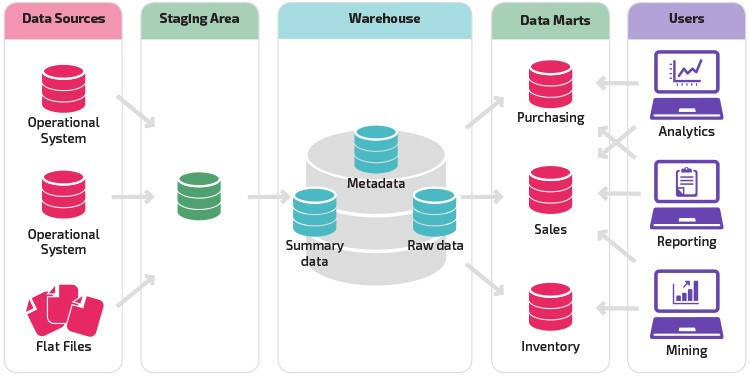
\includegraphics[width=0.8\linewidth]{IMAGE/DW-architecture.jpg}
    \caption{Kiến trúc của kho dữ liệu.}
    \label{fig:dw-architecture}
\end{figure}
\begin{enumerate}
    \item \textbf{Nguồn dữ liệu (Data Sources):} 
    Trong thực tế, dữ liệu hiếm khi nằm đồng nhất ở một nơi. Nguồn dữ liệu là lớp dưới cùng, nơi sản sinh hoặc chứa đựng dữ liệu gốc. Đối với hệ thống quản lý và phân tích chất lượng nước, dữ liệu có thể đến từ sự kết hợp của nhiều nguồn khác nhau:
    \begin{itemize}
        \item Các cơ sở dữ liệu quan hệ (RDBMS) của hệ thống quản lý trạm bơm hoặc phòng thí nghiệm (chứa thông tin mẫu thử, thời gian lấy mẫu).
        \item Dữ liệu từ các cảm biến IoT đo lường theo thời gian thực (được gọi qua các API API truyền tải dữ liệu JSON/XML về nhiệt độ, độ đục).
        \item Các tệp tin phẳng (Flat files) như CSV, Excel chứa dữ liệu ghi chép thủ công hoặc dữ liệu quan trắc lịch sử từ các cơ quan môi trường.
    \end{itemize}

    \item \textbf{Khu vực trung gian (Staging Area):} 
    Đây là vùng lưu trú tạm thời (landing zone) chuyên dùng để chứa dữ liệu thô vừa được trích xuất (Extract) từ các nguồn dữ liệu đa dạng kể trên. Mục đích chính của Staging Area là tạo ra một bộ đệm để thực hiện các tác vụ làm sạch và biến đổi dữ liệu (Transform) mà không gây áp lực tính toán lên các hệ thống nguồn OLTP đang vận hành. Tại đây, các kỹ sư dữ liệu sẽ thực hiện các thao tác quan trọng như:
    \begin{itemize}
        \item Xử lý các giá trị khuyết thiếu (Missing values), ví dụ như điền khuyết (imputation) cho các chỉ số pH hay Sulfate bị trống trong dữ liệu gốc.
        \item Loại bỏ các bản ghi trùng lặp và phát hiện các giá trị ngoại lai (Outliers) có thể làm sai lệch mô hình.
        \item Đồng nhất định dạng thời gian và quy đổi các đơn vị đo lường hóa lý về một chuẩn duy nhất.
    \end{itemize}

    \item \textbf{Kho lưu trữ trung tâm (Data Warehouse):} 
    Sau khi dữ liệu đã được làm sạch và chuẩn hóa hoàn toàn ở Staging Area, chúng sẽ được nạp (Load) vào kho lưu trữ trung tâm. Đây là trái tim của hệ thống, nơi lưu trữ toàn bộ dữ liệu lịch sử một cách có cấu trúc, tối ưu hóa cho các truy vấn phân tích phức tạp. Dữ liệu tại đây thường được mô hình hóa đa chiều (Dimensional Modeling) theo các lược đồ phổ biến:
    \begin{itemize}
        \item \textit{Star Schema (Lược đồ ngôi sao):} Cấu trúc phi chuẩn hóa, bao gồm một bảng Sự kiện trung tâm (Fact Table) lưu trữ các chỉ số định lượng (như nồng độ hóa chất, độ đục, độ cứng của nước) liên kết với các bảng Chiều (Dimension Tables) chứa thông tin mô tả (như thời gian, địa điểm, trạm quan trắc). Lược đồ này cho tốc độ truy vấn tương đối nhanh.
        \item \textit{Snowflake Schema (Lược đồ bông tuyết):} Là biến thể chuẩn hóa của Star Schema, trong đó các bảng Dimension được phân rã thành các bảng nhỏ hơn để tiết kiệm không gian lưu trữ, dù tốc độ truy vấn có thể chậm hơn đôi chút do phải kết nối (\texttt{JOIN}) nhiều bảng.
    \end{itemize}

    \item \textbf{Lớp trình bày dữ liệu (Information Delivery/Data Presentation):} 
    Đây là lớp giao tiếp cuối cùng, đóng vai trò phân phối dữ liệu từ kho lưu trữ trung tâm đến người dùng cuối hoặc các hệ thống nghiệp vụ khác. Tùy thuộc vào nhu cầu sử dụng, lớp này cung cấp các thành phần sau:
    \begin{itemize}
        \item \textbf{Data Mart:} Thay vì cho phép người dùng truy cập toàn bộ kho dữ liệu khổng lồ, Data Mart tạo ra các kho dữ liệu con, được trích xuất và tối ưu riêng cho từng nhóm đối tượng cụ thể. Ví dụ: một Data Mart chuyên biệt về 11Chỉ số an toàn nước'' dành riêng cho nhóm kỹ sư phát triển mô hình Machine Learning.
        \item \textbf{Công cụ phân tích và Trực quan hóa (BI Tools):} Kết nối với các nền tảng Business Intelligence (như Power BI, Tableau) để tạo ra các \textit{dashboard} theo dõi chất lượng nước theo thời gian thực.
        \item \textbf{Hệ thống Machine Learning:} Lớp này cung cấp nguồn dữ liệu đầu vào (đã được dán nhãn, làm sạch và tổng hợp) có độ tin cậy cao nhất để huấn luyện các thuật toán học máy như Support Vector Machine (SVM) hay Random Forest, từ đó dự đoán độ an toàn (Potability) của các mẫu nước mới trong tương lai.
    \end{itemize}
\end{enumerate}


\newpage

\subsection{Một số khái niệm khác}

\subsubsection{Quy trình ETL trong kho dữ liệu}
Quy trình ETL (Extract - Transform - Load) đóng vai trò cốt lõi trong kiến trúc của mọi hệ thống kho dữ liệu. Đặc biệt đối với các dự án ứng dụng học máy, chất lượng dữ liệu đầu vào là yếu tố quyết định trực tiếp đến độ chính xác của mô hình theo nguyên lý ``Garbage in, garbage out'' (Dữ liệu đầu vào kém sẽ tạo ra kết quả sai lệch). Do đó, ETL đảm nhiệm nhiệm vụ thiết yếu: sàng lọc, làm sạch và chuẩn hóa dữ liệu thô, từ đó kiến tạo một nền tảng dữ liệu đáng tin cậy trước khi bước vào giai đoạn phân tích chuyên sâu. Quy trình này được chia thành 3 giai đoạn chính:

\begin{itemize}
    \item \textbf{Extract (Trích xuất dữ liệu):} 
    Đây là bước thu thập dữ liệu thô từ các hệ thống nguồn và đưa vào khu vực trung gian (Staging Area). Trong phạm vi bài toán này, nguồn dữ liệu chủ yếu là tệp CSV tĩnh (ví dụ: tập dữ liệu Water Potability từ Kaggle). Bước trích xuất cần đảm bảo đọc chính xác các kiểu dữ liệu ban đầu, xử lý lỗi định dạng tệp (nếu có) và không làm thất thoát các bản ghi.
    
    \item \textbf{Transform (Biến đổi và làm sạch dữ liệu):} 
    Đây là công đoạn phức tạp và tốn nhiều công sức nhất. Dữ liệu thô về chất lượng nước thường chứa nhiều khiếm khuyết và không đồng nhất. Các thao tác biến đổi chính bao gồm:
    \begin{itemize}
        \item \textit{Xử lý giá trị khuyết (Handling Missing Values):} Các chỉ số như độ pH, nồng độ Sulfate hay Trihalomethanes thường xuyên bị thiếu hụt do lỗi thiết bị đo đạc. Tại đây, ta áp dụng các kỹ thuật điền khuyết (imputation) như dùng giá trị trung bình (mean), trung vị (median) hoặc các thuật toán nội suy.
        \item \textit{Phân nhóm dữ liệu (Binning/Discretization):} Biến đổi các giá trị số liên tục thành các biến danh mục (categorical) để dễ dàng tạo các bảng Chiều (Dimension). Ví dụ: phân dải giá trị độ pH thành các nhóm ``Tính Axit'', ``Trung tính'', ``Tính Kiềm''; hoặc chia chỉ số Hardness thành ``Nước mềm'', ``Nước cứng'' và ``Nước rất cứng''.
        \item \textit{Chuẩn hóa (Standardization):} Scale các giá trị (ví dụ: tổng chất rắn hòa tan Solids có giá trị lên tới hàng chục ngàn, trong khi Chloramines chỉ ở mức nhỏ hơn 10) về cùng một dải phân phối để tối ưu hóa cho các mô hình học máy.
    \end{itemize}
    
    \item \textbf{Load (Nạp dữ liệu):} 
    Sau khi dữ liệu đã được làm sạch và được định hình, chúng sẽ được nạp vào kho lưu trữ trung tâm theo cấu trúc Lược đồ ngôi sao (Star Schema). Quá trình này bao gồm việc nạp dữ liệu vào các bảng Chiều (Dim Tables) để tạo các khóa thay thế (Surrogate Keys), sau đó thực hiện tra cứu khóa (Lookup) để liên kết và nạp các giá trị đo lường cùng khóa ngoại vào bảng Sự kiện (Fact Table).
\end{itemize}

\subsubsection{Quá trình phân tích đa chiều (OLAP)}
Nếu ETL là công cụ để xây dựng kho, thì OLAP (Online Analytical Processing) là công cụ để khai thác kho dữ liệu đó. OLAP cho phép người dùng (nhà phân tích, nhà nghiên cứu) tương tác, khám phá và xoay lật khối dữ liệu (Data Cube) theo nhiều góc độ khác nhau một cách nhanh chóng, từ đó tìm ra các mẫu (patterns) ẩn sâu bên trong dữ liệu chất lượng nước. Các thao tác OLAP cơ bản bao gồm:

\begin{itemize}
    \item \textbf{Drill-down (Đi sâu vào chi tiết):} 
    Thao tác này cho phép người dùng đi từ mức độ tổng hợp cao xuống mức độ chi tiết hơn bằng cách hạ cấp các bậc của một chiều (Hierarchy). Ví dụ: từ việc xem tổng số mẫu nước không đạt chuẩn theo "Năm", người dùng có thể drill-down để xem chi tiết theo "Tháng", "Ngày" hoặc đi sâu từ phân loại "Nước cứng" xuống xem cụ thể nồng độ Canxi và Magie chi tiết của từng mẫu.
    
    \item \textbf{Roll-up (Tổng hợp dữ liệu):} 
    Ngược lại với Drill-down, Roll-up thực hiện gom nhóm dữ liệu chi tiết lên một cấp độ khái quát hơn. Ví dụ: gom nhóm hàng ngàn mẫu nước thử nghiệm độc lập lại để tính ra giá trị trung bình của nồng độ Sulfate hay lượng Carbon hữu cơ theo từng tháng, giúp dễ dàng nhận diện xu hướng thay đổi chất lượng nước trong dài hạn.
    
    \item \textbf{Slice (Cắt lát dữ liệu):} 
    Trích xuất ra một "lát cắt" của khối dữ liệu bằng cách chọn một giá trị duy nhất cho một chiều nhất định. Ví dụ: ta chỉ muốn lọc ra và phân tích tất cả các mẫu nước được gán nhãn là "An toàn để uống" (Potability = 1), để xem phân phối của các chất hóa học bên trong nhóm nước an toàn này trông như thế nào.
    
    \item \textbf{Dice (Đổ xắc/Cắt khối):} 
    Mở rộng của Slice, thao tác Dice cho phép thiết lập bộ lọc trên hai hoặc nhiều chiều cùng lúc để lấy ra một khối dữ liệu nhỏ hơn. Ví dụ: truy vấn để lấy ra tập hợp các mẫu nước vừa đáp ứng tiêu chí "Nước có tính Axit" (chiều pH), vừa nằm trong nhóm "Độ đục cao" (chiều Turbidity) và "Không an toàn" (chiều Potability) để phân tích sự cộng hưởng của các yếu tố rủi ro.
    
    \item \textbf{Pivot (Xoay trục):} 
    Thao tác thay đổi góc nhìn của báo cáo bằng cách xoay các trục dữ liệu (đổi từ hàng sang cột và ngược lại), giúp người phân tích có cái nhìn trực quan hơn khi muốn so sánh song song các thuộc tính với nhau.
\end{itemize}





\subsection{Phương pháp khai phá dữ liệu}

Để dự đoán tính an toàn của nước (Potability) dựa trên các chỉ số hóa lý, nhóm thực hiện huấn luyện và đánh giá trên 04 mô hình học máy hiện đại. Các mô hình này được lựa chọn nhằm tối ưu hóa khả năng phân loại trên tập dữ liệu có độ nhiễu cao và nhiều giá trị khuyết thiếu.

% RANDOM FOREST 
\subsubsection{Rừng ngẫu nhiên (Random Forest)}

\textbf{\large G}\textbf{iới thiệu} 

Trong nhiều tình huống ra quyết định thực tiễn, việc lựa chọn phương án tối ưu dựa trên thông tin tổng hợp từ tập thể thường cho kết quả đáng tin cậy hơn so với việc chỉ dựa vào một nguồn duy nhất. Khái niệm Rừng ngẫu nhiên \textit{(Random Forest)} ra đời từ ý tưởng rằng sự đa dạng trong các mô hình riêng lẻ, khi được tổng hợp, dẫn đến một kết quả tổng quát hóa tốt hơn so với bất kỳ mô hình đơn lẻ nào, một nguyên tắc được gọi là khả năng tổng hợp thông minh \textit{(wisdom of crowds)}. Mô hình sử dụng kỹ thuật ``bagging'' để huấn luyện từng cây trên một tập con ngẫu nhiên của dữ liệu. Cách tiếp cận này giúp cải thiện độ chính xác tổng thể của mô hình bằng cách giảm thiểu hiện tượng quá khớp và biến thiên. Khác với một cây quyết định đơn lẻ, rừng ngẫu nhiên dựa vào hai yếu tố ngẫu nhiên hóa trong quá trình huấn luyện (mẫu dữ liệu và tập thuộc tính), từ đó tăng tính tổng quát hóa và cải thiện độ ổn định của mô hình.  

\begin{figure}[H]
    \centering
    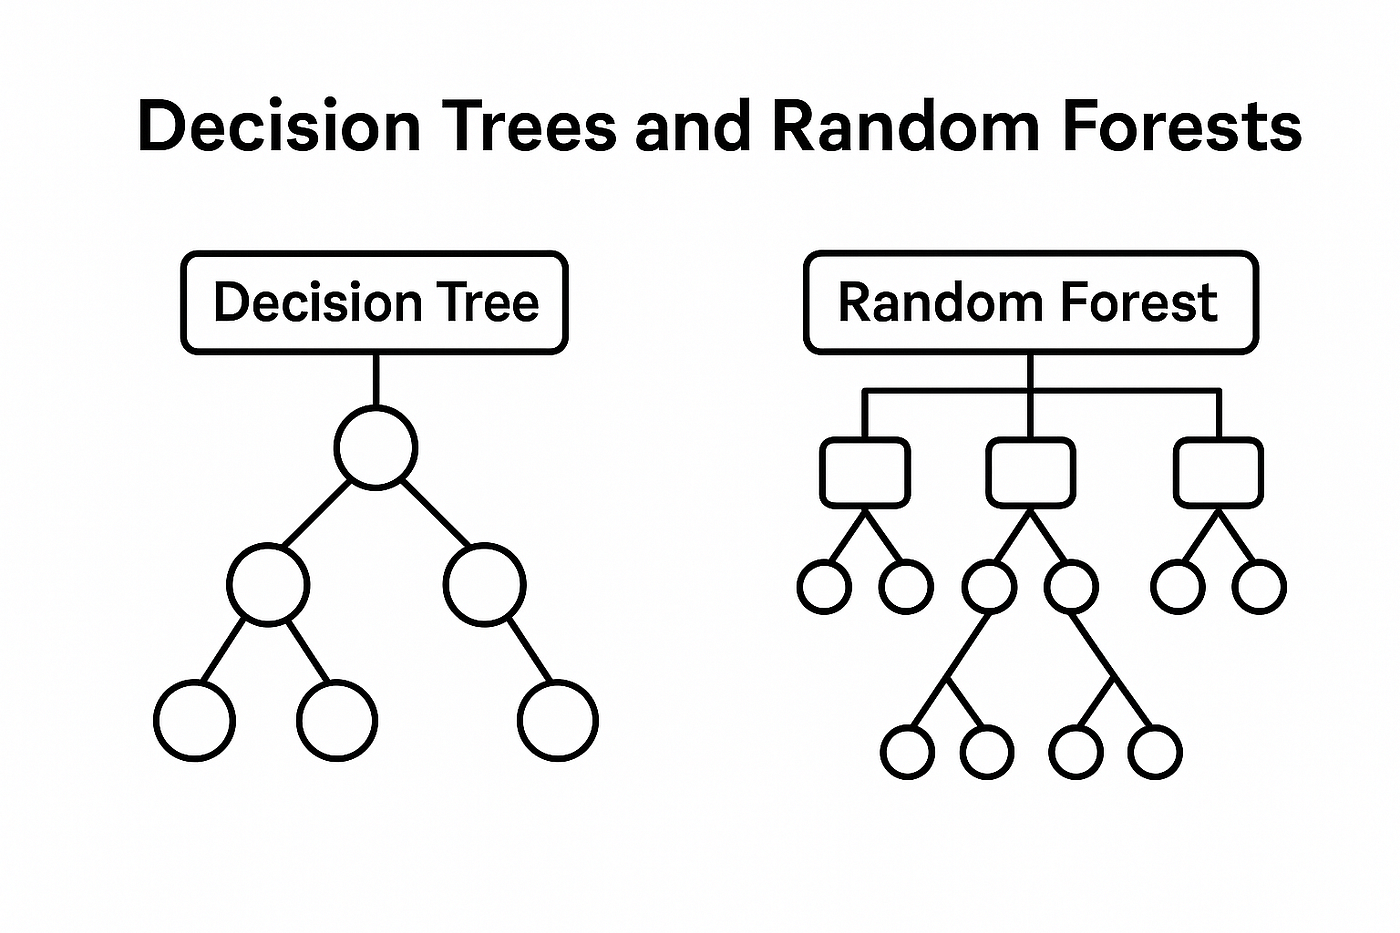
\includegraphics[width=0.5\linewidth]{IMAGE/random forest.png}
    \caption{Cây quyết định và rừng ngẫu nhiên.}
\end{figure}
\textbf{\large K}\textbf{hái niệm} 

Rừng ngẫu nhiên (\textit{Random Forest}) là một mô hình học có giám sát được phát triển nhằm giải quyết các bài toán phân lớp và hồi quy với hiệu suất vượt trội so với mô hình cây quyết định (\textit{Decision Tree}) đơn lẻ. Tương tự như một khu rừng được hình thành từ nhiều cây, mô hình này bao gồm một tập các cây quyết định được xây dựng độc lập, mỗi cây được huấn luyện trên một tập dữ liệu con được tạo ngẫu nhiên từ tập dữ liệu huấn luyện ban đầu. Các dự đoán từ từng cây thành phần sau đó được tổng hợp lại - thông qua cơ chế bỏ phiếu đa số trong bài toán phân lớp hoặc trung bình hóa trong bài toán hồi quy - để tạo ra kết quả cuối cùng. 


Đặc trưng ``ngẫu nhiên''  trong rừng ngẫu nhiên được thể hiện qua hai yếu tố chính, đóng vai trò cốt lõi trong việc tối ưu hóa hiệu suất mô hình:
\begin{itemize}
    \item \textbf{Ngẫu nhiên hóa tập dữ liệu huấn luyện:} Quá trình này được thực hiện thông qua kỹ thuật \textit{bootstrapping}, một phương pháp lấy mẫu có lặp lại từ tập dữ liệu huấn luyện ban đầu. Mỗi tập dữ liệu con được tạo ra ngẫu nhiên, cho phép một số điểm dữ liệu xuất hiện nhiều lần trong cùng một tập, trong khi các điểm khác có thể bị loại bỏ. Kỹ thuật này, thường được gọi là \textit{bagging (bootstrap aggregating)}, đảm bảo rằng mỗi cây quyết định trong rừng được huấn luyện trên một tập con khác nhau, từ đó tăng cường tính đa dạng và giảm thiểu \textit{biến thiên} trong dự đoán. Sự lặp lại của các điểm dữ liệu trong quá trình lấy mẫu giúp mô hình thích nghi với các mẫu đặc trưng, đồng thời hạn chế tác động của nhiễu dữ liệu, một yếu tố quan trọng trong việc cải thiện độ tổng quát hóa.
    \item \textbf{Ngẫu nhiên hóa tập con thuộc tính:} Trong quá trình phân chia các nút nội bộ (\textit{internal node}) của mỗi cây quyết định, chỉ một tập con ngẫu nhiên của các thuộc tính được xem xét thay vì toàn bộ tập thuộc tính. Số lượng thuộc tính trong tập con thường được đặt bằng căn bậc hai của tổng số thuộc tính ban đầu, một quy tắc được đề xuất bởi Breiman để cân bằng giữa tính đa dạng và hiệu quả tính toán. Chẳng hạn, nếu tập dữ liệu có 16 thuộc tính, chỉ khoảng 4 thuộc tính được chọn ngẫu nhiên tại mỗi nút để xác định ngưỡng phân chia. Phương pháp này không chỉ tăng cường tính độc lập giữa các cây mà còn giảm nguy cơ quá khớp bằng cách hạn chế sự phụ thuộc vào một tập thuộc tính cố định.
\end{itemize}
Sự kết hợp của hai yếu tố ngẫu nhiên hóa kể trên tạo nên một mô hình có khả năng học linh hoạt từ dữ liệu phức tạp, đồng thời duy trì độ ổn định và độ chính xác cao hơn so với một cây quyết định đơn lẻ. Tuy vậy, việc lựa chọn các tham số như số lượng cây trong rừng hoặc kích thước tập con thuộc tính cần được cân nhắc cẩn trọng, nhằm tránh làm gia tăng chi phí tính toán mà không mang lại cải thiện đáng kể về hiệu suất.

\textbf{\large R}\textbf{ừng ngẫu nhiên khắc phục nhược điểm của cây quyết định} 

Cây quyết định là một mô hình học có giám sát được sử dụng phổ biến trong lĩnh vực học máy nhờ tính dễ hiểu và khả năng biểu diễn trực quan các quy tắc phân loại. Tuy nhiên, mô hình này còn tồn tại một số hạn chế đáng kể, ảnh hưởng đến hiệu quả áp dụng trong các bài toán quy mô lớn hoặc đòi hỏi độ chính xác cao. Một trong những nhược điểm quan trọng nhất của cây quyết định là hiện tượng quá khớp, đặc biệt khi dữ liệu huấn luyện có nhiều biến động hoặc nhiễu. Cây quyết định thường có xu hướng ghi nhớ chi tiết các đặc điểm cụ thể của tập huấn
luyện, và do đó có thể dẫn đến mô hình phù hợp quá mức với dữ liệu đã thấy, nhưng lại không tổng quát tốt với các dữ liệu mới, chưa thấy.

Ngoài ra, cây quyết định cũng có thể bị thiên lệch nếu dữ liệu huấn luyện không đủ đa dạng hoặc có sự phân bố không đồng đều của các lớp. Điều này có thể dẫn đến việc cây quyết định chỉ học được các quy tắc phân chia mà không phản ánh đúng được sự phân bố của dữ liệu tổng thể.

Cuối cùng, cây quyết định có thể gặp phải vấn đề không ổn định, tức là thay đổi nhỏ trong dữ liệu huấn luyện có thể dẫn đến sự thay đổi lớn trong cấu trúc của cây. Điều này làm cho cây quyết định có thể trở nên khá nhạy cảm với những thay đổi trong tập huấn luyện và gây khó khăn trong việc xây dựng mô hình đáng tin cậy.

Để khắc phục những hạn chế trên, rừng ngẫu nhiên được đề xuất như một phương pháp tiên tiến, tận dụng sự kết hợp của nhiều cây quyết định để nâng cao hiệu suất và khả năng thích nghi. Mô hình này xây dựng một tập hợp các cây quyết định song song, mỗi cây được huấn luyện trên một tập dữ liệu con ngẫu nhiên, và kết quả cuối cùng được tổng hợp thông qua cơ chế bỏ phiếu đa số (\textit{majority voting}) cho phân lớp hoặc trung bình hóa cho hồi quy. Sự cải tiến này không chỉ giải quyết các nhược điểm của cây quyết định mà còn mở ra tiềm năng ứng dụng trong các bài toán quy mô lớn. Rừng ngẫu nhiên có thể giải quyết các vấn đề của cây quyết định bằng cách:
\begin{itemize}
    \item \textit{Giảm hiện tượng quá khớp:} Việc huấn luyện nhiều cây quyết định trên các mẫu dữ liệu khác nhau giúp rừng ngẫu nhiên giảm thiểu hiện tượng quá khớp. Mỗi cây được xây dựng dựa trên một tập con khác biệt của dữ liệu (thông qua quá trình \textit{bootstrapping}), do đó mô hình tổng thể ít bị ảnh hưởng bởi các điểm dữ liệu nhiễu hoặc ngoại lai.
    \item \textit{Tăng tính đa dạng và độ ổn định:} Bằng cách sử dụng nhiều cây quyết định được huấn luyện trên các tập dữ liệu và tập thuộc tính khác nhau, rừng ngẫu nhiên có khả năng học từ các khía cạnh khác nhau của dữ liệu. Điều này giúp tạo ra một mô hình ổn định hơn và ít nhạy cảm với các biến động nhỏ trong tập huấn luyện.
    \item \textit{Tối ưu hóa quá trình chọn thuộc tính:} Thay vì sử dụng toàn bộ tập thuộc tính tại mỗi nút phân chia, rừng ngẫu nhiên chỉ lựa chọn ngẫu nhiên một tập con các thuộc tính. Chiến lược này giúp giảm thiểu sự thiên lệch trong việc học và tăng khả năng tổng quát hóa của mô hình.
    \item \textit{Hiệu suất thực nghiệm cao:} Trong nhiều bài toán thực tế, rừng ngẫu nhiên đạt được hiệu suất rất cao và thường khó bị vượt qua. Nhờ cơ chế bỏ phiếu, các cây quyết định có hiệu suất thấp hoặc bị quá khớp sẽ có ảnh hưởng hạn chế đến kết quả cuối cùng, trong khi các cây mạnh được ưu tiên. Việc kết hợp nhiều cây chất lượng cao giúp cải thiện độ chính xác phân loại so với việc sử dụng một cây quyết định đơn lẻ.
\end{itemize}

\textbf{\large G}\textbf{iải thuật}

\setcounter{algocf}{1} % Thiết lập bắt đầu từ Algorithm 2 (nếu bạn muốn hiện số 3.2 thì tuỳ chỉnh ở file chính)

\begin{algorithm}[H]
\DontPrintSemicolon
\caption{\texttt{RandomForestTrain} - Huấn luyện mô hình Random Forest}

\Input{ Tập huấn luyện $(X, Y)$ gồm $N$ mẫu;\newline
        Số lượng cây $B$;\newline
        Số đặc trưng ngẫu nhiên tại mỗi node: $m$}
\Output{ Tập hợp các cây $\{f_1, f_2, \dots, f_B\}$}

Khởi tạo rừng rỗng: $\mathcal{F} \leftarrow \emptyset$;\;

\For{$b = 1$ \KwTo $B$}{
    Lấy mẫu bootstrap $(X_b, Y_b)$ từ $(X, Y)$ bằng cách chọn $N$ mẫu có hoàn lại;\;
    
    Huấn luyện cây $f_b$ trên $(X_b, Y_b)$ với:\;\\
    \nonl \Indp $\bullet$ Tại mỗi node: chọn ngẫu nhiên $m$ đặc trưng và chia theo đặc trưng tốt nhất\; \Indm
    
    Thêm $f_b$ vào rừng: $\mathcal{F} \leftarrow \mathcal{F} \cup \{f_b\}$;\;
}
\textbf{return} $\mathcal{F}$\;
\end{algorithm}
\begin{algorithm}[H]
\DontPrintSemicolon
\caption{\texttt{RandomForestPredict} - Dự đoán với mô hình Random Forest}

\Input{ Mẫu mới $x$;\newline
        Tập huấn luyện $(X, Y)$;\newline
        Số cây $B$, số đặc trưng ngẫu nhiên $m$}
\Output{ Dự đoán $\hat{y}$}

Huấn luyện mô hình: $\mathcal{F} \leftarrow \texttt{RandomForestTrain}(X, Y, B, m)$;\;

Lấy dự đoán từ từng cây: $\hat{y}_b \leftarrow f_b(x), \quad \forall f_b \in \mathcal{F}$;\;

\textbf{return} \textit{Biểu quyết đa số (classification)} hoặc \textit{trung bình (regression)} của $\{\hat{y}_1, \dots, \hat{y}_B\}$\;
\end{algorithm}




\textbf{\large C}\textbf{ông thức} 

Dự đoán cuối cùng ($\hat{y}$) được xác định bằng cách lấy biểu quyết đa số từ các cây thành phần ($f_b$):
\begin{equation}
\hat{y} = \arg\max_y \sum_{b=1}^{B} I(f_b(x) = y)
\end{equation}
Trong đó $I(\cdot)$ là hàm chỉ thị và $B$ là số lượng cây trong rừng.

\subsubsection{Support Vector Machine (SVM)}

\textbf{\large G}\textbf{iới thiệu}

Trong số các thuật toán học máy được sử dụng cho bài toán này, thuật toán \textit{Support Vector Machine(SVM)} nổi bật như một phương pháp mạnh mẽ và hiệu quả, đặc biệt trong các bài toán phân loại nhị phân như phân biệt nguồn nước an toàn và không an toàn. Thuật toán này hoạt động bằng cách tìm một siêu phẳng (\textit{hyperplane}) trong không gian đặc trưng để tách biệt hai lớp với khoảng cách biên (margin) lớn nhất, đảm bảo khả năng tổng quát hóa tốt ngay cả khi dữ liệu mẫu nước có sự chồng chéo hoặc nhiễu. Điểm mạnh của SVM nằm ở khả năng xử lý các tập dữ liệu có chiều cao, chẳng hạn như các chỉ số hóa lý đa dạng của nước, và khả năng sử dụng kỹ thuật kernel để xử lý các trường hợp dữ liệu không tách biệt tuyến tính. Hơn nữa, SVM hỗ trợ khả năng điều chỉnh tham số, chẳng hạn như tham số C để cân bằng giữa lỗi phân loại và tối ưu hóa biên, giúp mô hình thích nghi tốt với các đặc trưng phức tạp của dữ liệu đánh giá chất lượng nước.

\textbf{\large K}\textbf{hái niệm} 

Thuật toán SVM là một phương pháp \textit{học máy có giám sát} được sử dụng chủ yếu cho các bài toán phân loại nhị phân (\textit{binary classification}), dù cũng có thể mở rộng cho phân loại đa lớp hoặc hồi quy. SVM hoạt động bằng cách xây dựng một siêu phẳng (hyperplane), là một không gian con $n-1$ chiều trong không gian đặc trưng n chiều, nhằm tách biệt hai lớp dữ liệu một cách tối ưu. Trong không gian hai chiều, siêu phẳng này là một đường thẳng phân chia mặt phẳng thành hai vùng, mỗi vùng đại diện cho một lớp dữ liệu.

Tính tối ưu của siêu phẳng được xác định thông qua việc tối đa hóa khoảng cách biên (\textit{margin}), tức là khoảng cách từ siêu phẳng đến các vector hỗ trợ (\textit{support vectors}) - các điểm dữ liệu gần nhất của mỗi lớp. Khoảng cách này thường được tính dựa trên độ đo Euclidean trong không gian đặc trưng, và khoảng cách biên lớn hơn giúp mô hình tổng quát hóa tốt hơn, giảm nguy cơ quá khớp khi dự đoán trên dữ liệu mới. Trong quá trình huấn luyện, SVM sử dụng tập dữ liệu có nhãn để xác định siêu phẳng tối ưu bằng cách giải bài toán tối ưu hóa, đảm bảo sự phân tách rõ ràng giữa các lớp.

Khi dữ liệu không thể tách biệt tuyến tính trong không gian đặc trưng ban đầu, SVM áp dụng kỹ thuật kernel để ánh xạ dữ liệu vào một không gian chiều cao hơn, nơi các lớp có thể được tách biệt. Tham số C trong SVM được sử dụng để điều chỉnh mức độ khoan dung đối với lỗi phân loại, cân bằng giữa tối ưu hóa khoảng cách biên và độ chính xác trên tập huấn luyện, giúp xử lý dữ liệu có nhiễu.

\begin{figure}[H]
    \centering
    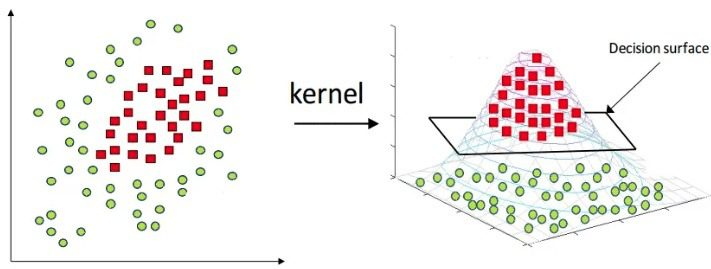
\includegraphics[width=0.5\linewidth]{IMAGE/kernel.jpg}
    \caption{Ánh xạ không gian đặc trưng bằng hàm kernel.}
\end{figure}
Sau khi huấn luyện, SVM phân loại dữ liệu mới bằng cách xác định vị trí của chúng trong không gian đặc trưng, dựa trên khoảng cách từ điểm dữ liệu đến siêu phẳng. Với khả năng xử lý các không gian đặc trưng cao chiều và dữ liệu phức tạp, SVM được ứng dụng rộng rãi trong các bài toán như nhận diện nguồn nước an toàn/không an toàn, phân loại văn bản, nhận diện hình ảnh, và phát hiện gian lận trong an ninh mạng.

\textbf{\large C}\textbf{ông thức và giải thuật}

%\textbf{1. Mô hình SVM cơ bản và Kí hiệu}

Trong bài toán phân loại nhị phân, tập dữ liệu huấn luyện bao gồm các cặp $(x^{(i)},y^{(i)})$, với $x^{(i)}\in\mathbb{R}^{n}$ là vector đặc trưng và nhãn lớp $y^{(i)}\in\{-1,1\}$. Việc sử dụng nhãn $\{-1,1\}$ giúp đơn giản hóa biểu diễn toán học của siêu phẳng phân chia $w^{T}x+b=0$. Bộ phân loại tuyến tính này được tham số hóa bởi vector trọng số $w\in\mathbb{R}^{n}$ và tham số chặn $b\in\mathbb{R}$. 

Hàm phân loại dự đoán được xác định như sau:
\begin{equation}
h_{w,b}(x)=\text{sign}(w^{T}x+b)
\end{equation}
Trong đó, $\text{sign}(z)=1$ nếu $z\ge0$ và $\text{sign}(z)=-1$ nếu $z<0$.

%\textbf{2. Hàm khoảng cách và Khoảng cách hình học}
Mục tiêu cốt lõi của giải thuật SVM là tìm một siêu phẳng tối ưu có khoảng cách biên (margin) lớn nhất. Khoảng cách này được tính từ siêu phẳng đến các vector hỗ trợ (support vectors) - là các điểm dữ liệu nằm gần nhất của mỗi lớp. 
\begin{itemize}
    \item Khoảng cách hình học (geometric margin) từ một điểm dữ liệu $x^{(i)}$ đến siêu phẳng được tính theo công thức: $\gamma^{(i)}=y^{(i)}\left(\left(\frac{w}{||w||_2}\right)^{T}x^{(i)}+\frac{b}{||w||_2}\right)$.
    \item Khoảng cách biên tổng giữa hai lớp là $\frac{2}{||w||}$. Để tối đa hóa khoảng cách biên này, giải thuật cần tối thiểu hóa đại lượng $||w||$, hay tương đương là tối thiểu hóa $\frac{1}{2}||w||^{2}$ để đảm bảo hàm mục tiêu là hàm lồi và dễ tính đạo hàm.
\end{itemize}
%\textbf{3. Bài toán tối ưu hóa dạng gốc (Primal Form)}

Giả sử tập dữ liệu có thể phân tách tuyến tính, bài toán tối ưu hóa tìm siêu phẳng phân chia của SVM được phát biểu dưới dạng:
\begin{equation}
\min_{w,b}\frac{1}{2}||w||^{2}
\end{equation}
Với điều kiện ràng buộc: $y^{(i)}(w^{T}x^{(i)}+b)\ge1$, với $i=1,2,...,m$.

Ràng buộc này đảm bảo mọi điểm dữ liệu đều được phân loại đúng và nằm ngoài hoặc nằm ngay trên lề (margin). Các điểm thỏa mãn đẳng thức $y^{(i)}(w^{T}x^{(i)}+b)=1$ chính là các vector hỗ trợ.
%\textbf{4. Bài toán đối ngẫu Lagrange (Dual Form)}

Khi số chiều đặc trưng $n$ lớn hoặc tập dữ liệu không thể phân tách tuyến tính, việc giải bài toán đối ngẫu mang lại hiệu quả cao hơn. Bằng cách áp dụng phương pháp nhân tử Lagrange, bài toán gốc được chuyển sang dạng đối ngẫu như sau:
\begin{equation}
\max_{\alpha}\sum_{i=1}^{m}\alpha_{i}-\frac{1}{2}\sum_{i,j=1}^{m}\alpha_{i}\alpha_{j}y^{(i)}y^{(j)}(x^{(i)})^{T}x^{(j)}
\end{equation}
Với các ràng buộc: 
\begin{itemize}
    \item $\alpha_{i}\ge0$, với $i=1,...,m$
    \item $\sum_{i=1}^{m}\alpha_{i}y^{(i)}=0$
\end{itemize}

Trong đó, $\alpha_i$ là các nhân tử Lagrange. Từ bài toán đối ngẫu, vector trọng số $w$ của siêu phẳng có thể được xác định lại thông qua công thức: $w=\sum_{i=1}^{m}\alpha_{i}y^{(i)}x^{(i)}$. Theo điều kiện Karush-Kuhn-Tucker (KKT), chỉ những vector hỗ trợ mới có $\alpha_i > 0$, do đó giải thuật chỉ cần dựa vào một số lượng nhỏ các vector hỗ trợ này để phân tách dữ liệu, giúp tiết kiệm bộ nhớ và tăng tốc độ tính toán.
% \textbf{5. Giải quyết dữ liệu phi tuyến với Hàm Kernel (Kernel Trick)}

Trong trường hợp dữ liệu không thể phân tách tuyến tính trong không gian ban đầu, SVM áp dụng kỹ thuật hàm kernel để ánh xạ dữ liệu vào một không gian đặc trưng nhiều chiều ($d$-chiều) nơi tồn tại siêu phẳng phân tách được hai lớp. 

Hàm mục tiêu đối ngẫu chỉ phụ thuộc vào tích vô hướng $(x^{(i)})^{T}x^{(j)}$, do đó có thể thay thế tích vô hướng này bằng hàm Kernel $K(x, z) = \phi(x)^T \phi(z)$ mà không cần tính toán trực tiếp ánh xạ đặc trưng $\phi(x)$. Một số hàm Kernel phổ biến được sử dụng bao gồm:
\begin{itemize}
    \item \textbf{Đa thức kernel (Polynomial kernel):} $K(x, z)=(x^{T}z+c)^{d}$
    \item \textbf{Gaussian kernel (hay RBF kernel):} $K(x, z)=\exp\left(-\frac{||x-z||^{2}}{2\sigma^{2}}\right)$
\end{itemize}
Mô hình tối ưu hóa hàm đối ngẫu Lagrange để xác định siêu phẳng phân cách:
\begin{equation}
L(\alpha) = \sum_{i=1}^{m} \alpha_i - \frac{1}{2} \sum_{i,j=1}^{m} \alpha_i \alpha_j y^{(i)} y^{(j)} K(x^{(i)}, x^{(j)})
\end{equation}
Trong đó, $\alpha_i$ là các nhân tử Lagrange và $K(x^{(i)}, x^{(j)})$ là hàm kernel giúp xử lý các mối quan hệ phi tuyến tính.

% \subsection{Mạng nơ-ron nhân tạo (Artificial Neural Network - ANN)}

% \textbf{\large G}\textbf{iới thiệu}

% Trong những thập kỷ gần đây, sự bùng nổ của dữ liệu lớn (Big Data) và sự tiến bộ vượt bậc của năng lực tính toán đã tạo điều kiện cho Mạng thần kinh nhân tạo (Artificial Neural Network - ANN) trở thành một trong những mô hình học máy mạnh mẽ và được ứng dụng rộng rãi nhất. Nằm trong nhánh Học sâu (Deep Learning), ANN đã chứng minh được sự ưu việt trong việc giải quyết các bài toán phức tạp mà các mô hình học máy truyền thống thường gặp khó khăn, chẳng hạn như nhận dạng hình ảnh, xử lý ngôn ngữ tự nhiên, phân tích chuỗi thời gian và các bài toán phân loại có tính phi tuyến tính cao. Sự linh hoạt và khả năng tự động học hỏi các biểu diễn đặc trưng (feature representations) từ dữ liệu thô đã đưa ANN trở thành nền tảng cho nhiều hệ thống trí tuệ nhân tạo hiện đại.

% \textbf{\large K}\textbf{hái niệm}

% Mạng thần kinh nhân tạo là một mô hình toán học và tính toán được thiết kế lấy cảm hứng từ cấu trúc và cơ chế hoạt động của mạng lưới hệ thần kinh sinh học trong não bộ con người. Cấu trúc cơ bản của một ANN bao gồm nhiều nút xử lý thông tin, được gọi là các nơ-ron nhân tạo (artificial neurons) hoặc perceptron, được tổ chức thành các lớp (layers) kết nối với nhau. Một kiến trúc ANN truyền thống (Feedforward Neural Network) thường bao gồm ba thành phần chính được minh họa trong Hình \ref{fig:ANN}:

% \begin{figure}[H]
%     \centering
%     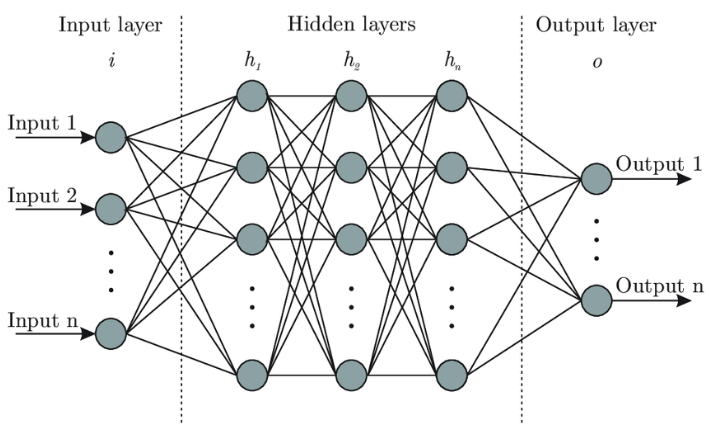
\includegraphics[width=0.5\linewidth]{IMAGE/ANN-1.png}
%     \caption{Mạng nơ-ron nhân tạo gồm lớp đầu vào, các lớp ẩn trung gian và lớp đầu ra.}
%     \label{fig:ANN}
% \end{figure}
% \begin{itemize}
%     \item \textbf{Lớp đầu vào (Input Layer):} Là nơi tiếp nhận dữ liệu ban đầu. Số lượng nơ-ron trong lớp này tương ứng với số lượng đặc trưng (features) của tập dữ liệu đầu vào.
%     \item \textbf{Các lớp ẩn (Hidden Layers):} Nằm giữa lớp đầu vào và lớp đầu ra, có nhiệm vụ trích xuất và học hỏi các quy luật, đặc trưng phi tuyến tính phức tạp ẩn sâu trong dữ liệu. Một mạng có thể có một hoặc nhiều lớp ẩn; số lượng lớp và số lượng nơ-ron trong mỗi lớp ảnh hưởng trực tiếp đến khả năng học (capacity) của mô hình.
%     \item \textbf{Lớp đầu ra (Output Layer):} Đưa ra kết quả dự đoán cuối cùng. Tùy thuộc vào loại bài toán, số lượng nơ-ron và hàm kích hoạt ở lớp này sẽ thay đổi (ví dụ: 1 nơ-ron với hàm Sigmoid cho bài toán phân loại nhị phân, hoặc nhiều nơ-ron với hàm Softmax cho bài toán phân loại đa lớp).
% \end{itemize}

% Thông tin trong ANN truyền thống chỉ di chuyển theo một hướng duy nhất: từ lớp đầu vào, qua các lớp ẩn, đến lớp đầu ra. Quá trình này được gọi là lan truyền tiến (Forward Propagation).

% \textbf{\large C}\textbf{ông thức tính toán tại mỗi nơ-ron}

% Tại mỗi nơ-ron trong các lớp ẩn và lớp đầu ra, dữ liệu đầu vào được xử lý thông qua hai phép toán cơ bản: tính tổng có trọng số (weighted sum) và áp dụng hàm kích hoạt (activation function).

% Giả sử một nơ-ron nhận $n$ tín hiệu đầu vào từ lớp trước đó, ký hiệu là $x_1, x_2, \dots, x_n$. Mỗi kết nối giữa các nơ-ron đều được gán một trọng số (weight) $w_i$, thể hiện mức độ quan trọng của tín hiệu đầu vào tương ứng. Ngoài ra, mỗi nơ-ron còn có một hệ số chệch (bias) $b$ giúp dịch chuyển đồ thị của hàm kích hoạt, tăng tính linh hoạt cho mô hình.

% Tổng có trọng số $z$ tại nơ-ron được tính bằng công thức:
% \begin{equation}
% z = \sum_{i=1}^{n} w_i x_i + b = \mathbf{w}^T \mathbf{x} + b
% \end{equation}

% Sau đó, giá trị $z$ này được truyền qua một hàm kích hoạt phi tuyến $f$ để tạo ra giá trị đầu ra $y$ của nơ-ron đó:
% \begin{equation}
% y = f(z) = f\left( \sum_{i=1}^{n} w_i x_i + b \right)
% \end{equation}

% Hàm kích hoạt đóng vai trò then chốt trong việc đưa tính phi tuyến vào mô hình, giúp ANN có khả năng học được các hàm phức tạp. Nếu không có hàm kích hoạt phi tuyến, một mạng ANN nhiều lớp cũng chỉ tương đương với một mô hình hồi quy tuyến tính đơn giản. Một số hàm kích hoạt phổ biến bao gồm:
% \begin{figure}[H]
%     \centering
    
%     % Đồ thị 1: ReLU
%     \begin{tikzpicture}
%         \begin{axis}[
%             width=5.5cm, height=5.5cm,
%             title={\textbf{ReLU}: $f(z) = \max(0, z)$},
%             axis lines=middle,
%             xmin=-5, xmax=5,
%             ymin=-1, ymax=5,
%             samples=100,
%             domain=-5:5,
%             grid=both,
%             grid style={line width=.1pt, draw=gray!30},
%             enlargelimits={abs=0.2}
%         ]
%         \addplot[blue, thick] {max(0, x)};
%         \end{axis}
%     \end{tikzpicture}
%     \hfill
%     % Đồ thị 2: Sigmoid
%     \begin{tikzpicture}
%         \begin{axis}[
%             width=5.5cm, height=5.5cm,
%             title={\textbf{Sigmoid}: $f(z) = \frac{1}{1 + e^{-z}}$},
%             axis lines=middle,
%             xmin=-5, xmax=5,
%             ymin=-0.2, ymax=1.2,
%             samples=100,
%             domain=-5:5,
%             grid=both,
%             grid style={line width=.1pt, draw=gray!30},
%             enlargelimits={abs=0.1}
%         ]
%         \addplot[red, thick] {1 / (1 + exp(-x))};
%         \end{axis}
%     \end{tikzpicture}
%     \hfill
%     % Đồ thị 3: Tanh
%     \begin{tikzpicture}
%         \begin{axis}[
%             width=5.5cm, height=5.5cm,
%             title={\textbf{Tanh}: $f(x) = \frac{e^z - e^{-z}}{e^z + e^{-z}}$},
%             axis lines=middle,
%             xmin=-5, xmax=5,
%             ymin=-1.2, ymax=1.2,
%             samples=100,
%             domain=-5:5,
%             grid=both,
%             grid style={line width=.1pt, draw=gray!30},
%             enlargelimits={abs=0.1}
%         ]
%         \addplot[green!60!black, thick] {tanh(x)};
%         \end{axis}
%     \end{tikzpicture}
    
%     \caption{Đồ thị các hàm kích hoạt phổ biến: ReLU, Sigmoid và Tanh.}
%     \label{fig:activation_functions}
% \end{figure}
% \begin{itemize}
%     \item \textbf{ReLU:} $f(z) = \max(0, z)$, phổ biến nhất trong các lớp ẩn vì tính toán nhanh và khắc phục được hiện tượng triệt tiêu đạo hàm (vanishing gradient).
%     \item \textbf{Sigmoid:} $f(z) = \frac{1}{1 + e^{-z}}$, nén giá trị đầu ra vào khoảng $(0, 1)$, thường dùng ở lớp đầu ra cho phân loại nhị phân.
%     \item \textbf{Tanh:} $f(z) = \frac{e^z - e^{-z}}{e^z + e^{-z}}$, nén giá trị vào khoảng $(-1, 1)$, thường hội tụ nhanh hơn Sigmoid.
% \end{itemize}

% \textbf{\large G}\textbf{iải thuật}

% Quá trình huấn luyện một mạng ANN thực chất là quá trình tối ưu hóa các tham số (trọng số $w$ và bias $b$) sao cho sai số giữa giá trị dự đoán của mạng và giá trị thực tế của dữ liệu huấn luyện là nhỏ nhất. Sai số này được đo lường bằng một Hàm mất mát (Loss Function), ví dụ như Mean Squared Error (MSE) cho bài toán hồi quy hoặc Binary Cross-Entropy (BCE) cho bài toán phân loại nhị phân.

% Giải thuật cốt lõi để huấn luyện ANN là \textbf{Lan truyền ngược (Backpropagation)} kết hợp với các thuật toán tối ưu hóa dựa trên \textbf{Đạo hàm giảm dần (Gradient Descent)}. Quy trình này diễn ra lặp đi lặp lại qua nhiều kỷ nguyên (epochs) với các bước chính như sau:

% \begin{enumerate}
%     \item \textbf{Lan truyền thuận (Forward Propagation):} Đưa một mẫu dữ liệu (hoặc một lô - batch dữ liệu) vào lớp đầu vào, tính toán qua các lớp ẩn để đưa ra kết quả dự đoán ở lớp đầu ra.
%     \item \textbf{Tính toán hàm mất mát (Compute Loss):} So sánh kết quả dự đoán với nhãn thực tế để tính toán giá trị của Hàm mất mát $L$.
%     \item \textbf{Lan truyền ngược (Backpropagation):} Bắt đầu từ lớp đầu ra, áp dụng quy tắc chuỗi (chain rule) trong vi tích phân để tính toán đạo hàm riêng (gradient) của Hàm mất mát theo từng trọng số và bias trong mạng: $\frac{\partial L}{\partial w_{ij}}$ và $\frac{\partial L}{\partial b_i}$. Gradient này cho biết mỗi tham số đóng góp bao nhiêu vào sai số tổng thể.
%     \item \textbf{Cập nhật trọng số (Weight Update):} Sử dụng thuật toán Gradient Descent (hoặc các biến thể cải tiến như Adam, RMSprop) để điều chỉnh các trọng số và bias theo hướng làm giảm hàm mất mát. Công thức cập nhật cơ bản là:
%     \begin{equation}
%     w_{ij} := w_{ij} - \eta \frac{\partial L}{\partial w_{ij}}
%     \end{equation}
%     \begin{equation}
%     b_i := b_i - \eta \frac{\partial L}{\partial b_i}
%     \end{equation}
%     Trong đó, $\eta$ là Tốc độ học (Learning rate), một siêu tham số quyết định bước nhảy của thuật toán trong không gian tối ưu.
% \end{enumerate}
% % ==========================================
% % 1. SƠ ĐỒ LAN TRUYỀN THUẬN (FORWARD PROPAGATION)
% % ==========================================
% \begin{figure}[H]
%     \centering
%     \begin{tikzpicture}[
%         scale=0.7, transform shape, % Thu nhỏ tỷ lệ xuống 0.7
%         input/.style={circle, draw=blue!70, thick, fill=blue!10, minimum size=1.2cm},
%         bias/.style={circle, draw=gray!70, thick, fill=gray!10, minimum size=1.2cm},
%         neuron/.style={circle split, draw=green!70!black, thick, fill=green!10, minimum size=3.5cm, align=center},
%         output/.style={circle, draw=orange!70, thick, fill=orange!10, minimum size=1.2cm},
%         loss/.style={rectangle, draw=red!70, thick, fill=red!10, minimum size=1.2cm, rounded corners},
%         arrow/.style={-Stealth, thick, draw=black!80},
%         label/.style={midway, fill=white, inner sep=2pt, font=\small}
%     ]

%         % Khai báo các Nút (Nodes)
%         \node[input] (x1) at (0, 3) {$x_1$};
%         \node[input] (x2) at (0, 1) {$x_2$};
%         \node (dots) at (0, -0.5) {$\vdots$};
%         \node[input] (xn) at (0, -2) {$x_n$};
%         \node[bias] (b)  at (0, 5) {$1$};

%         % Nơ-ron trung tâm (Chia làm 2 nửa: Tính tổng và Kích hoạt)
%         \node[neuron] (n) at (6, 1) {$z = \sum_{i=1}^n w_i x_i + b$ \nodepart{lower} $y = f(z)$};

%         % Output và Loss
%         \node[output] (y) at (10, 1) {$y$};
%         \node[loss] (L) at (13, 1) {$L(y, y_{true})$};

%         % Vẽ các mũi tên (Forward)
%         \draw[arrow] (x1) -- (n.160) node[label] {$w_1$};
%         \draw[arrow] (x2) -- (n.180) node[label] {$w_2$};
%         \draw[arrow] (xn) -- (n.200) node[label] {$w_n$};
%         \draw[arrow] (b)  -- (n.145) node[label] {$b$};

%         \draw[arrow] (n.0) -- (y) node[label] {};
%         \draw[arrow] (y) -- (L) node[label] {Tính Loss};

%     \end{tikzpicture}
%     \caption{Quá trình Lan truyền thuận (Forward Propagation) tại một Nơ-ron nhân tạo.}
%     \label{fig:forward_prop}
% \end{figure}

% % ==========================================
% % 2. SƠ ĐỒ LAN TRUYỀN NGƯỢC (BACKWARD PROPAGATION)
% % ==========================================
% \begin{figure}[H]
%     \centering
%     \begin{tikzpicture}[
%         scale=0.7, transform shape, % Thu nhỏ tỷ lệ xuống 0.7
%         input/.style={circle, draw=blue!70, thick, fill=blue!10, minimum size=1.2cm},
%         bias/.style={circle, draw=gray!70, thick, fill=gray!10, minimum size=1.2cm},
%         neuron/.style={circle split, draw=green!70!black, thick, fill=green!10, minimum size=3.5cm, align=center},
%         output/.style={circle, draw=orange!70, thick, fill=orange!10, minimum size=1.2cm},
%         loss/.style={rectangle, draw=red!70, thick, fill=red!10, minimum size=1.2cm, rounded corners},
%         backarrow/.style={Stealth-, thick, red, dashed},
%         label/.style={midway, fill=white, inner sep=2pt, font=\small, text=red}
%     ]

%         % Vị trí các Nút giống hệt bên trên
%         \node[input] (x1) at (0, 3) {$x_1$};
%         \node[input] (x2) at (0, 1) {$x_2$};
%         \node (dots) at (0, -0.5) {$\vdots$};
%         \node[input] (xn) at (0, -2) {$x_n$};
%         \node[bias] (b)  at (0, 5) {$1$};

%         % Nơ-ron lúc này hiển thị gradient của Z
%         \node[neuron] (n) at (6, 1) {$\frac{\partial L}{\partial z} = \frac{\partial L}{\partial y} \cdot f'(z)$ \nodepart{lower} $y = f(z)$};

%         \node[output] (y) at (10, 1) {$y$};
%         \node[loss] (L) at (13, 1) {$L$};

%         % Làm mờ các đường Forward để làm nền
%         \begin{scope}[gray!30, -Stealth, thick]
%             \draw (x1) -- (n.160);
%             \draw (x2) -- (n.180);
%             \draw (xn) -- (n.200);
%             \draw (b)  -- (n.145);
%             \draw (n.0) -- (y);
%             \draw (y) -- (L);
%         \end{scope}

%         % Vẽ các đường Backward truyền đạo hàm (Màu đỏ, nét đứt, hơi uốn cong để không đè vạch cũ)
%         \draw[backarrow] (n.150) to[bend right=15] node[label] {$\frac{\partial L}{\partial w_1} = \frac{\partial L}{\partial z}x_1$} (x1.0);
%         \draw[backarrow] (n.175) to[bend right=15] node[label] {$\frac{\partial L}{\partial w_2} = \frac{\partial L}{\partial z}x_2$} (x2.0);
%         \draw[backarrow] (n.195) to[bend left=15]  node[label] {$\frac{\partial L}{\partial w_n} = \frac{\partial L}{\partial z}x_n$} (xn.0);
%         \draw[backarrow] (n.135) to[bend right=15] node[label] {$\frac{\partial L}{\partial b} = \frac{\partial L}{\partial z}$} (b.0);

%         \draw[backarrow] (n.30)  to[bend right=20] node[label] {$\frac{\partial L}{\partial y}$} (y.150);
%         \draw[backarrow] (y.30)  to[bend right=20] node[label] {$\frac{\partial L}{\partial y} = \nabla_y L$} (L.150);

%     \end{tikzpicture}
%     \caption{Quá trình Lan truyền ngược (Backward Propagation) tính Gradient tại một Nơ-ron nhân tạo.}
%     \label{fig:backward_prop}
% \end{figure}

% Quá trình này được lặp lại cho đến khi Hàm mất mát đạt đến một giá trị đủ nhỏ hoặc mô hình không còn cải thiện thêm, đánh dấu việc ANN đã "học" được cách biểu diễn dữ liệu và sẵn sàng để đưa ra dự đoán trên dữ liệu mới.

\subsubsection{XGBoost (Extreme Gradient Boosting)}

\textbf{\large G}\textbf{iới thiệu}

Trong lĩnh vực học máy, đặc biệt là khi làm việc với dữ liệu dạng bảng (tabular data), XGBoost (Extreme Gradient Boosting) được công nhận là một trong những thuật toán mạnh mẽ và gặt hái được nhiều thành công nhất. Được phát triển ban đầu bởi Tianqi Chen, XGBoost nhanh chóng thống trị các cuộc thi khoa học dữ liệu (như Kaggle) nhờ khả năng mang lại độ chính xác vượt trội và tốc độ thực thi cực nhanh. Sự kết hợp hoàn hảo giữa kỹ thuật học tập hợp (Ensemble Learning), khả năng tính toán song song (Parallel Processing), và các cơ chế chống quá khớp (Overfitting) đã giúp XGBoost trở thành sự lựa chọn hàng đầu cho cả các bài toán hồi quy lẫn phân lớp phức tạp.

\textbf{\large K}\textbf{hái niệm}

XGBoost là một phiên bản cải tiến tối ưu hóa của thuật toán Gradient Boosting. Thuật toán này hoạt động dựa trên nguyên lý kết hợp nhiều "mô hình học yếu" (weak learners) – thường là các cây quyết định (Decision Trees) – để tạo thành một "mô hình học mạnh" (strong learner). Quá trình này diễn ra một cách tuần tự (sequential): mỗi cây quyết định mới được xây dựng sẽ tập trung vào việc sửa chữa những sai lầm (residual errors) mà các cây trước đó đã mắc phải.

Điểm khác biệt cốt lõi khiến XGBoost trở nên "Extreme" (cực độ) so với Gradient Boosting truyền thống bao gồm:
\begin{itemize}
    \item \textbf{Tối ưu hóa đạo hàm bậc hai:} Sử dụng khai triển Taylor bậc hai (tính cả Gradient và Hessian) để xấp xỉ hàm mất mát, giúp mô hình hội tụ nhanh và chính xác hơn.
    \item \textbf{Chính quy hóa (Regularization):} Tích hợp sẵn các thành phần L1 (Lasso) và L2 (Ridge) vào hàm mục tiêu để kiểm soát cấu trúc của cây, phạt nặng các cây quá phức tạp, từ đó ngăn chặn hiệu quả hiện tượng quá khớp.
    \item \textbf{Nhận thức sự thưa thớt (Sparsity Awareness):} Tự động học được hướng rẽ tối ưu cho các giá trị khuyết thiếu (missing values) mà không cần phải điền khuyết trước.
\end{itemize}


\textbf{\large C}\textbf{ông thức toán học}

Giả sử mô hình bao gồm $K$ cây quyết định, giá trị dự đoán cuối cùng cho một mẫu $x_i$ là tổng dự đoán của tất cả các cây:
\begin{equation}
\hat{y}_i = \sum_{k=1}^{K} f_k(x_i), \quad f_k \in \mathcal{F}
\end{equation}
Trong đó, $\mathcal{F}$ là không gian của tất cả các cây quyết định.

Tại bước lặp thứ $t$, thuật toán cần tìm một cây $f_t$ mới để thêm vào mô hình nhằm tối thiểu hóa hàm mục tiêu (Objective Function). Hàm mục tiêu của XGBoost bao gồm hai phần: Hàm mất mát $\mathcal{L}$ (đo lường độ lệch giữa thực tế và dự đoán) và Thành phần chính quy hóa $\Omega$ (đo lường độ phức tạp của cây):
\begin{equation}
\text{Obj}^{(t)} = \sum_{i=1}^{n} l\left(y_i, \hat{y}_i^{(t-1)} + f_t(x_i)\right) + \Omega(f_t)
\end{equation}

Sử dụng khai triển Taylor bậc hai để xấp xỉ hàm mất mát, hàm mục tiêu được viết lại thành:
\begin{equation}
\text{Obj}^{(t)} \approx \sum_{i=1}^{n} \left[ g_i f_t(x_i) + \frac{1}{2} h_i f_t^2(x_i) \right] + \Omega(f_t)
\end{equation}
Với $g_i = \partial_{\hat{y}^{(t-1)}} l(y_i, \hat{y}^{(t-1)})$ là đạo hàm bậc một (Gradient) và $h_i = \partial^2_{\hat{y}^{(t-1)}} l(y_i, \hat{y}^{(t-1)})$ là đạo hàm bậc hai (Hessian) của hàm mất mát.

Thành phần chính quy hóa $\Omega(f_t)$ được định nghĩa bằng số lượng nút lá $T$ và bình phương trọng số $w$ của các nút lá đó:
\begin{equation}
\Omega(f_t) = \gamma T + \frac{1}{2} \lambda \sum_{j=1}^{T} w_j^2
\end{equation}

Từ đó, trọng số tối ưu $w_j^*$ cho nút lá $j$ và giá trị tối ưu của hàm mục tiêu có thể tính được bằng công thức:
\begin{equation}
w_j^* = -\frac{\sum_{i \in I_j} g_i}{\sum_{i \in I_j} h_i + \lambda}
\end{equation}

\textbf{\large G}\textbf{iải thuật huấn luyện}

Quá trình huấn luyện XGBoost thực chất là quá trình xây dựng từng cây quyết định để tối ưu hóa hàm mục tiêu nói trên. Giải thuật diễn ra qua các bước:

\begin{enumerate}
    \item \textbf{Khởi tạo:} Bắt đầu với một giá trị dự đoán cơ sở $\hat{y}_i^{(0)}$ (thường là trung bình của nhãn hoặc 0.5 đối với phân loại nhị phân).
    \item \textbf{Lặp qua $t = 1$ đến $K$ (số lượng cây):}
    \begin{itemize}
        \item Tính toán giá trị Gradient ($g_i$) và Hessian ($h_i$) cho từng điểm dữ liệu dựa trên kết quả dự đoán của bước $t-1$.
        \item \textbf{Xây dựng cây $f_t$ (Thuật toán Exact Greedy hoặc Histogram-based):} Thuật toán duyệt qua các đặc trưng để tìm điểm chia (split) tốt nhất. Mức độ "tốt" của một điểm chia được đánh giá bằng độ lợi (Gain):
        \begin{equation}
        \text{Gain} = \frac{1}{2} \left[ \frac{G_L^2}{H_L + \lambda} + \frac{G_R^2}{H_R + \lambda} - \frac{(G_L + G_R)^2}{H_L + H_R + \lambda} \right] - \gamma
        \end{equation}
        Trong đó, $G_L, G_R, H_L, H_R$ lần lượt là tổng Gradient và Hessian của nhánh trái và nhánh phải. Nếu $\text{Gain} > 0$, thuật toán sẽ thực hiện tách nhánh.
        \item Gán trọng số $w_j^*$ cho các lá của cây $f_t$ vừa xây dựng.
    \end{itemize}
    \item \textbf{Cập nhật dự đoán:} Thêm cây mới vào quần thể kết hợp với hệ số học (Learning rate - $\eta$) để ngăn chặn cây học quá nhanh (Shrinkage):
    \begin{equation}
    \hat{y}_i^{(t)} = \hat{y}_i^{(t-1)} + \eta f_t(x_i)
    \end{equation}
    \item \textbf{Điều kiện dừng:} Quá trình lặp kết thúc khi đạt đủ số lượng cây $K$ hoặc kích hoạt cơ chế dừng sớm (Early Stopping) nếu hiệu suất trên tập kiểm thử không còn được cải thiện.
\end{enumerate}

\newpage
\input{PHƯƠNG PHÁP KHAI PHÁ DỮ LIỆU}
\newpage
\section{Tiền xử lý và Khám phá dữ liệu (EDA)}

\subsection{Khám phá dữ liệu thô (Raw Data EDA)}
Trước khi tiến hành bất kỳ thao tác xử lý nào, nhóm thực hiện khảo sát trạng thái nguyên bản của tập dữ liệu \textbf{water\_potability.csv} để nhận diện các vấn đề về chất lượng dữ liệu.

\subsubsection{Tổng quan cấu trúc}
Bộ dữ liệu bao gồm 3.276 bản ghi với 10 đặc trưng hóa lý. Qua quan sát sơ bộ bằng lệnh \texttt{df.head()}, dữ liệu thô xuất hiện nhiều giá trị \textbf{NaN} (Not a Number) tại các cột quan trọng.

\subsubsection{Phân tích dữ liệu thiếu (Missing Values)}
Đây là vấn đề nghiêm trọng nhất của bộ dữ liệu này. Nhóm thực hiện thống kê số lượng dòng thiếu trên từng thuộc tính:

\begin{figure}[H]
    \centering
    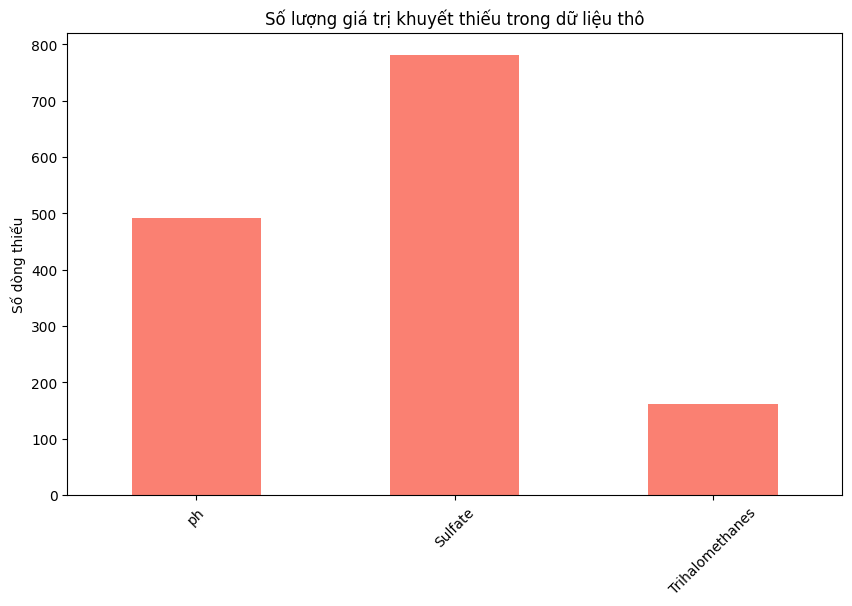
\includegraphics[width=0.7\textwidth]{IMAGE/raw_missing.png}
    \caption{Thống kê các cột bị khuyết thiếu dữ liệu trong tập thô}
    \label{fig:raw_missing}
\end{figure}

\textbf{Nhận xét:} Cột \textbf{Sulfate} bị khuyết nhiều nhất với hơn 700 dòng, tiếp đến là \textbf{ph} và \textbf{Trihalomethanes}. Nếu thực hiện xóa bỏ các dòng này, nhóm sẽ mất đi khoảng 30\% lượng dữ liệu huấn luyện, gây ảnh hưởng đến độ chính xác của mô hình AI.

\subsection{Quy trình Tiền xử lý dữ liệu (Data Preprocessing)}
Dựa trên các vấn đề đã nhận diện tại bước EDA thô, nhóm tiến hành xây dựng quy trình ETL (Extract - Transform - Load) tự động. Mục tiêu của quy trình này không chỉ là làm sạch dữ liệu mà còn tái cấu trúc thông tin để phù hợp với kiến trúc kho dữ liệu Star Schema.

\subsubsection{Làm sạch dữ liệu (Data Cleaning)}
Nhóm nhận diện có 3 thuộc tính quan trọng bị khuyết thiếu dữ liệu diện rộng: pH (491 dòng), Sulfate (781 dòng) và Trihalomethanes (162 dòng). Để bảo toàn dung lượng mẫu cho việc huấn luyện AI mà không làm thay đổi đặc tính thống kê chung, nhóm áp dụng phương pháp \textbf{Mean Imputation} (điền khuyết bằng giá trị trung bình) thông qua bước xử lý \texttt{If field value is null} trong Pentaho.

Các tham số cụ thể được thiết lập dựa trên giá trị trung bình tính toán từ tập mẫu sạch:
\begin{itemize}
    \item \textbf{Cột pH:} Điền giá trị $7.08$.
    \item \textbf{Cột Sulfate:} Điền giá trị $333.77$.
    \item \textbf{Cột Trihalomethanes:} Điền giá trị $66.39$.
\end{itemize}

\subsubsection{Kỹ thuật Đặc trưng và Phân nhóm (Feature Engineering - Binning)}
Đây là giai đoạn quan trọng nhất để chuyển đổi dữ liệu từ dạng số liên tục sang dạng danh mục, phục vụ cho việc phân tích đa chiều trong kho dữ liệu. Nhóm sử dụng bước \texttt{Number range} để phân loại các chỉ số dựa trên các tiêu chuẩn hóa lý:

\begin{itemize}
    \item \textbf{Phân loại nồng độ pH (Dim\_Acidity):}
    \begin{itemize}
        \item \textbf{Axit:} pH $< 6.5$.
        \item \textbf{Trung tính:} $6.5 \le \text{pH} \le 8.5$.
        \item \textbf{Kiềm:} pH $> 8.5$.
    \end{itemize}
    \item \textbf{Phân loại độ cứng (Dim\_Hardness):}
    \begin{itemize}
        \item \textbf{Nước mềm:} Hardness $< 60$ mg/L.
        \item \textbf{Nước cứng vừa:} $60 \le \text{Hardness} < 120$ mg/L.
        \item \textbf{Nước cứng:} $120 \le \text{Hardness} < 180$ mg/L.
        \item \textbf{Nước rất cứng:} Hardness $\ge 180$ mg/L.
    \end{itemize}
\end{itemize}

% \subsubsection{Hiện thực hóa quy trình ETL bằng Pentaho Data Integration}
% Để tự động hóa việc luân chuyển dữ liệu từ tập tin thô vào kho dữ liệu, nhóm sử dụng công cụ \textbf{Pentaho Data Integration (PDI)}. Toàn bộ logic tiền xử lý, biến đổi đặc trưng và quản lý khóa thay thế (Surrogate Keys) được đóng gói trong tệp luồng xử lý \texttt{water\_etl\_pipeline.ktr}.

% Quy trình xử lý dữ liệu trong Pentaho được thiết kế theo trình tự tuyến tính để đảm bảo tính toàn vẹn của dữ liệu qua từng bước:

% \begin{itemize}
%     \item \textbf{Dữ liệu đầu vào:} Trích xuất từ tệp CSV gốc thông qua step \texttt{CSV file input}.
%     \item \textbf{Xử lý giá trị khuyết thiếu:} Nhóm sử dụng step \texttt{If field value is null} để điền các giá trị trung bình đã tính toán: pH ($7.08$), Sulfate ($333.77$) và Trihalomethanes ($66.39$).
%     \item \textbf{Phân loại và Rời rạc hóa:} Các step \texttt{Number range} thực hiện logic chia ngưỡng cho độ pH và độ cứng của nước để tạo ra các danh mục đặc trưng.
%     \item \textbf{Quản lý bảng Dimension:} Sử dụng \texttt{Combination lookup/update} để sinh khóa Surrogate Key tự động, đảm bảo kho dữ liệu hoạt động ổn định và tối ưu hiệu suất truy vấn.
%     \item \textbf{Nạp dữ liệu vào bảng Fact:} Kết thúc bằng step \texttt{Table output} để nạp toàn bộ dữ liệu sạch vào bảng \texttt{Fact\_Water\_Sample} trong cơ sở dữ liệu.
% \end{itemize}

% \begin{figure}[H]
%     \centering
%     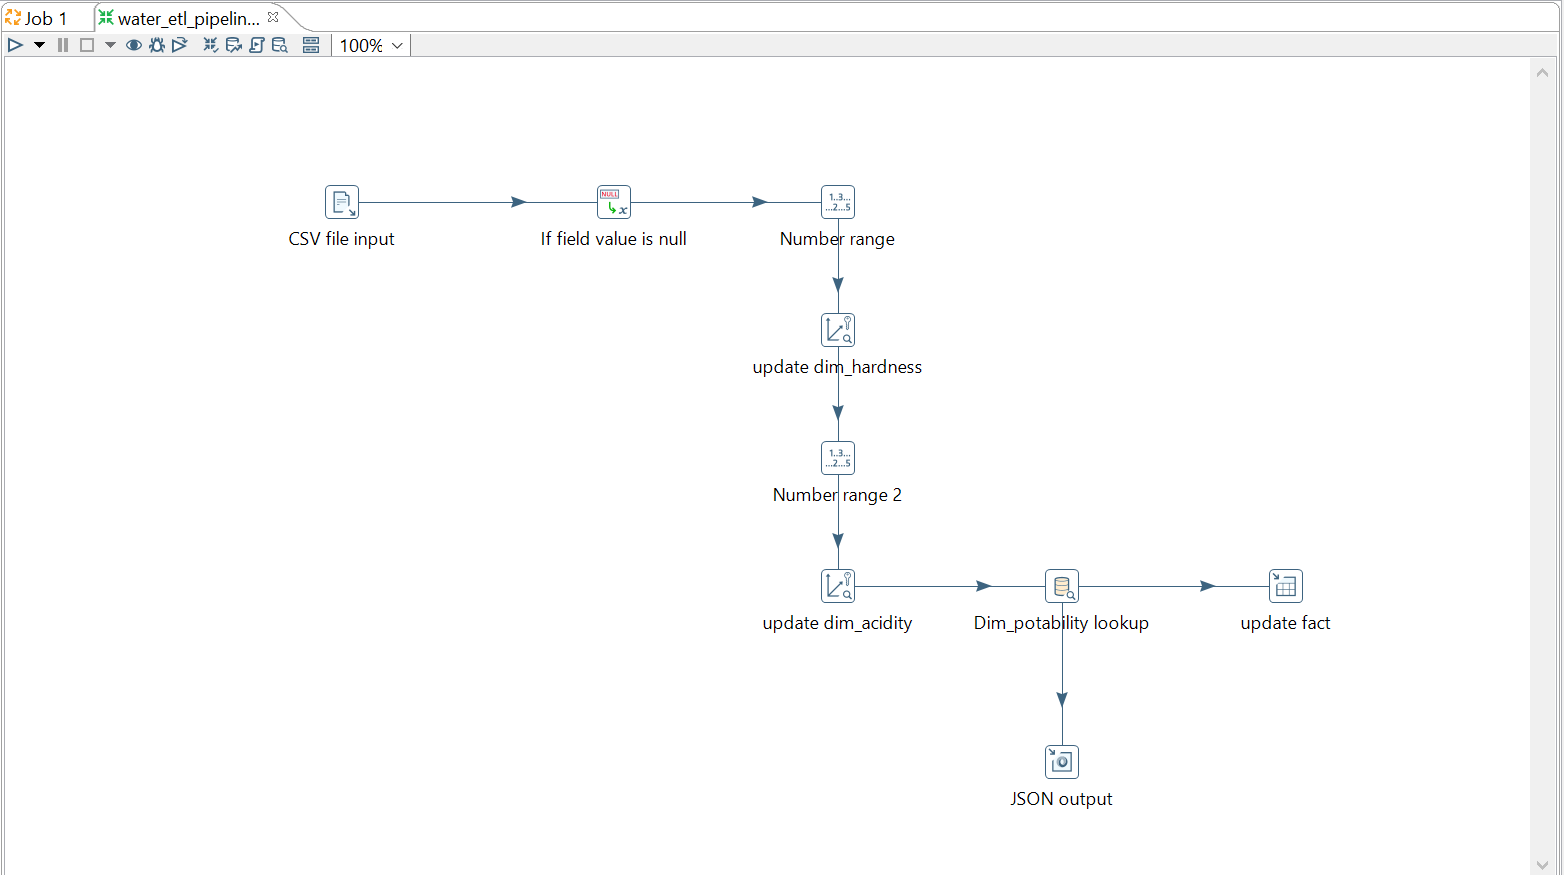
\includegraphics[width=1\textwidth]{IMAGE/pentaho_flow.png} 
%     \caption{Sơ đồ luồng xử lý dữ liệu tự động trong giao diện Pentaho}
%     \label{fig:pentaho_flow}
% \end{figure}

\subsection{Khám phá dữ liệu sau tiền xử lý (Clean Data EDA)}
Sau khi hoàn tất quy trình làm sạch và điền khuyết tại Mục 3.2, nhóm tiến hành phân tích chi tiết toàn bộ các chỉ số hóa lý. Đây là bước quan trọng để xác nhận dữ liệu đã sẵn sàng cho việc huấn luyện mô hình và xây dựng kho dữ liệu.

\subsubsection{Phân tích mối quan hệ đa biến (Correlation Matrix)}
Nhóm sử dụng ma trận tương quan để đánh giá lại mối liên hệ giữa các thuộc tính sau khi đã xử lý dữ liệu thiếu.

\begin{figure}[H]
    \centering
    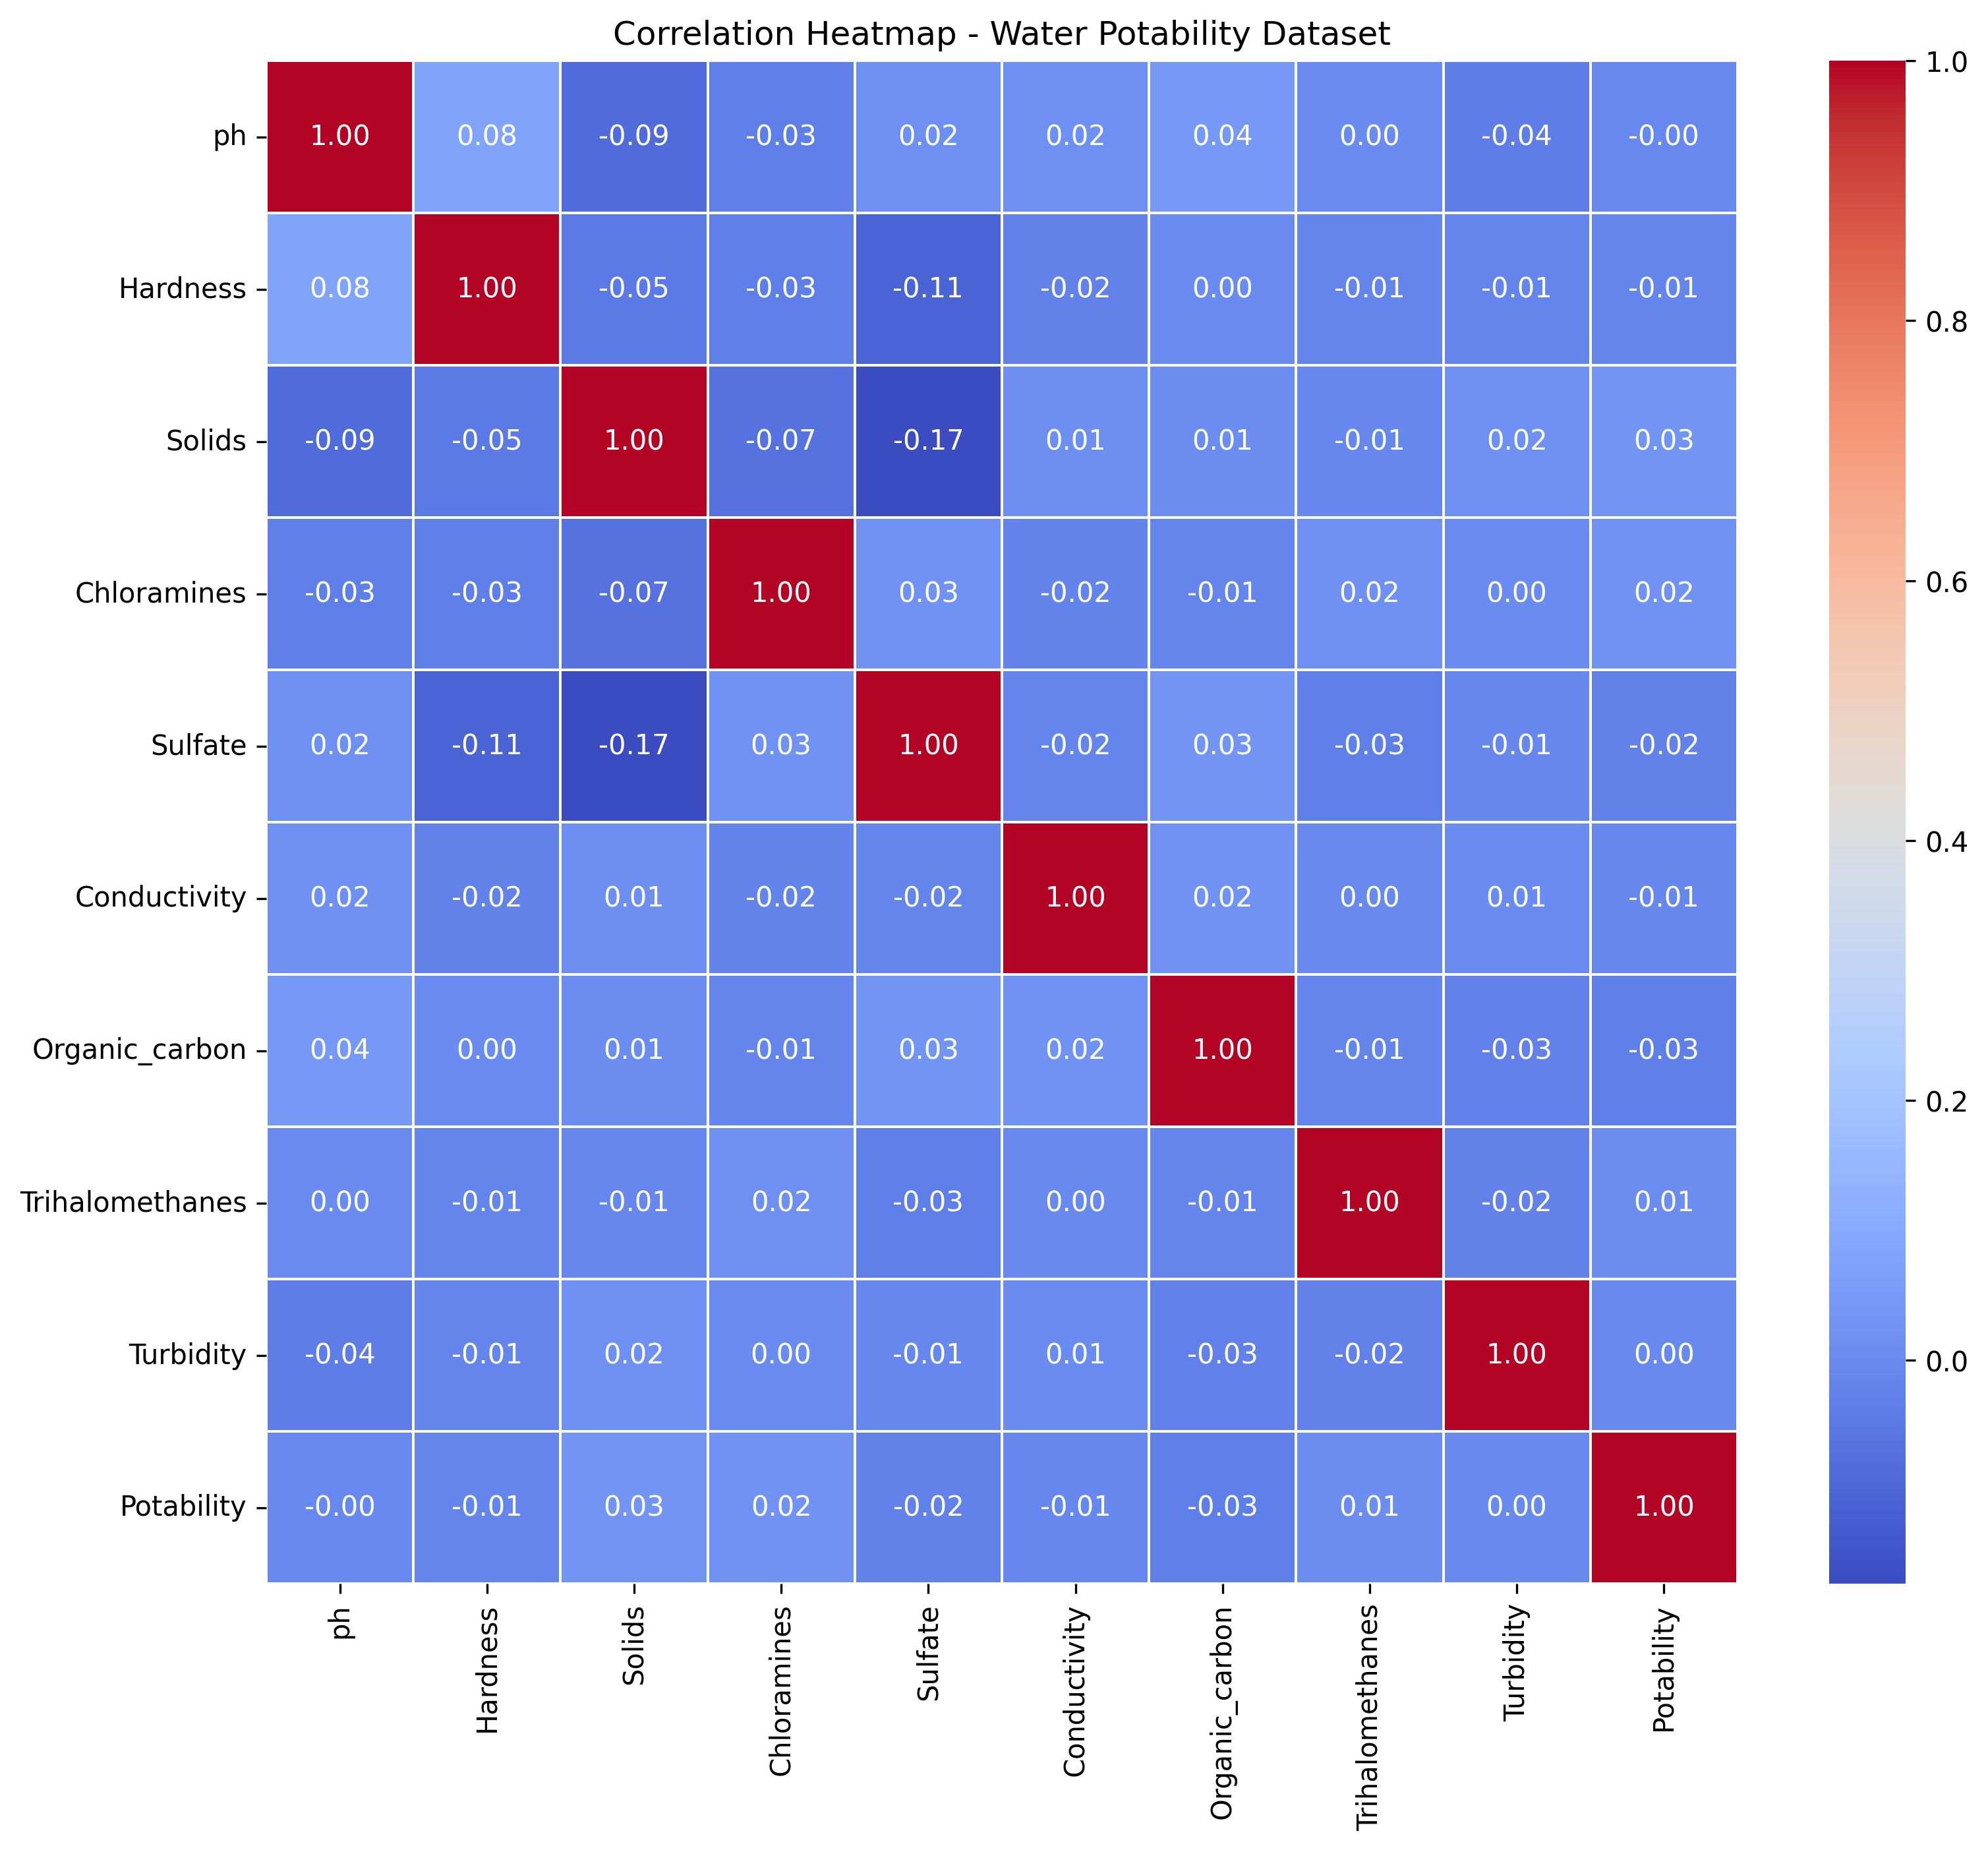
\includegraphics[width=0.8\textwidth]{IMAGE/heatmap.png}
    \caption{Ma trận tương quan của dữ liệu sau tiền xử lý}
\end{figure}

\textbf{Nhận xét:} Hầu hết các đặc trưng (pH, Hardness, Sulfate,...) đều có tương quan xấp xỉ bằng $0$ với nhãn Potability. Điều này minh chứng cho tính độc lập cao giữa các đặc trưng, tránh hiện tượng đa cộng tuyến và tạo điều kiện thuận lợi cho các thuật toán phi tuyến tính.

\subsubsection{Phân tích các biến rời rạc (Categorical Analysis)}
Sau khi thực hiện kỹ thuật Binning trong quy trình ETL để tạo ra các nhóm phân loại mới, nhóm tiến hành so sánh tỉ lệ an toàn (Potability) giữa các danh mục này để tìm kiếm các đặc điểm đặc trưng của nguồn nước an toàn.

\begin{figure}[H]
    \centering
    \begin{minipage}{0.48\textwidth}
        \centering
        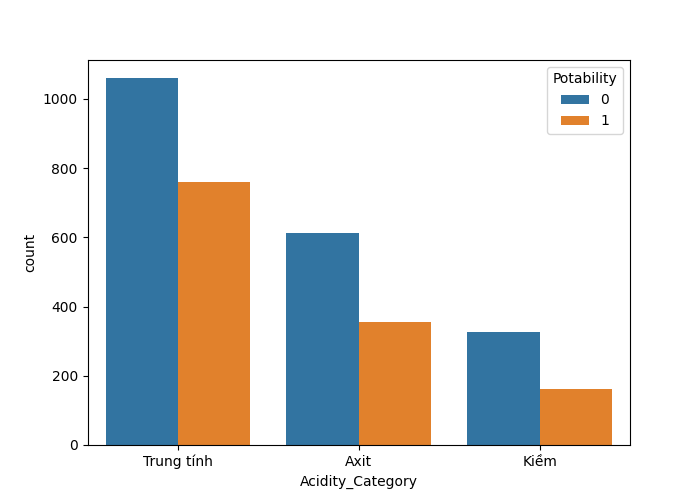
\includegraphics[width=1\textwidth]{IMAGE/discrete_acidity.png}
        \caption{Tỉ lệ Potability theo nồng độ pH (Dim\_Acidity)}
    \end{minipage}
    \hfill
    \begin{minipage}{0.48\textwidth}
        \centering
        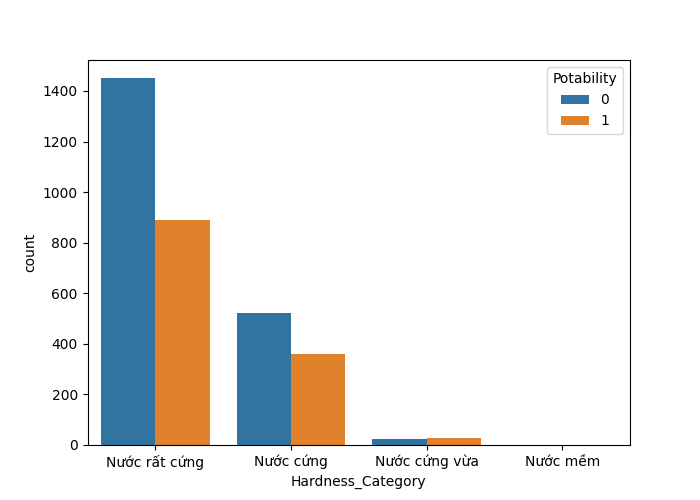
\includegraphics[width=1\textwidth]{IMAGE/discrete_hardness.png}
        \caption{Tỉ lệ Potability theo độ cứng (Dim\_Hardness)}
    \end{minipage}
\end{figure}

Qua các biểu đồ thống kê trên, nhóm rút ra các kết luận quan trọng phục vụ cho việc phân tích chất lượng nước:
\begin{itemize}
    \item \textbf{Về nồng độ pH (Acidity\_Category):} 
    \begin{itemize}
        \item Nhóm nước \textbf{Trung tính} chiếm tỷ trọng áp đảo với hơn 1.000 mẫu không an toàn và gần 800 mẫu an toàn. 
        \item Tiếp theo là nhóm nước \textbf{Axit} và cuối cùng là nhóm nước \textbf{Kiềm}. 
        \item Tỷ lệ giữa nước uống được (Potability = 1) và không uống được (Potability = 0) duy trì khá đồng nhất trên cả 3 phân loại, cho thấy tính axit hay kiềm đơn lẻ không phải là yếu tố quyết định sự khác biệt lớn về độ an toàn.
    \end{itemize}
    
    \item \textbf{Về độ cứng (Hardness\_Category):}
    \begin{itemize}
        \item Tập dữ liệu cho thấy một sự tập trung cực kỳ lớn vào nhóm \textbf{Nước rất cứng} (vượt mốc 1.400 mẫu ở nhãn 0).
        \item Nhóm \textbf{Nước cứng} đứng vị trí thứ hai với tổng số lượng mẫu đáng kể, trong khi nhóm \textbf{Nước cứng vừa} chiếm tỷ lệ rất thấp.
        \item Đặc biệt, nhóm \textbf{Nước mềm} gần như không xuất hiện hoặc chiếm số lượng không đáng kể trong tập dữ liệu này.
        \item Tương tự như pH, phân phối của nhãn Potability trên các nhóm độ cứng không có sự chênh lệch đột biến, củng cố giả thuyết về mối quan hệ phi tuyến tính phức tạp giữa các biến.
    \end{itemize}
\end{itemize}

\subsubsection{Phân tích chi tiết các biến liên tục}
Nhóm thực hiện trực quan hóa phân phối cho từng biến để kiểm chứng tác động của quy trình ETL và nhận diện đặc tính dữ liệu sạch.

\paragraph{Biến "ph":} \leavevmode\\
\begin{figure}[H]
    \centering
    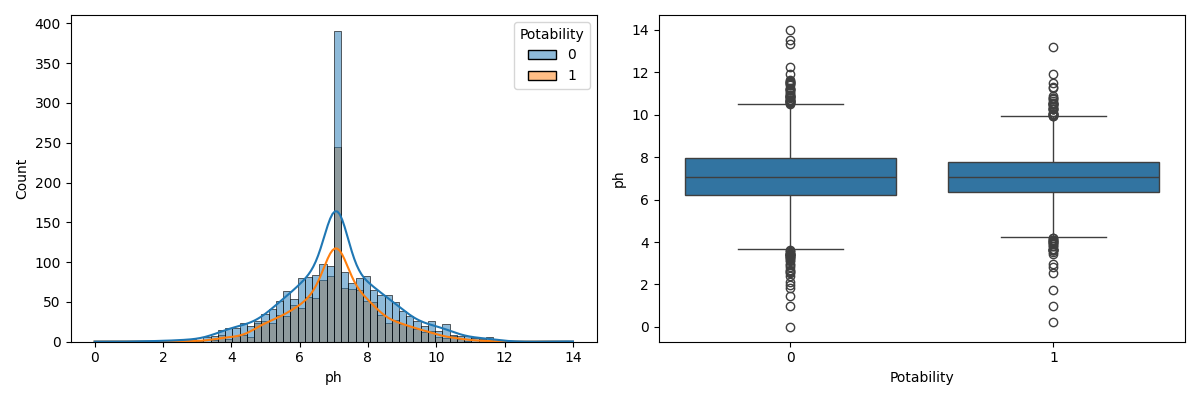
\includegraphics[width=0.9\textwidth]{IMAGE/dist_ph.png}
    \caption{Phân phối và biểu đồ hộp của biến ph sau khi điền khuyết}
\end{figure}

\textbf{Nhận xét:} Biểu đồ cho thấy pH có phân phối chuẩn, tập trung mạnh quanh giá trị trung bình $7.0$. Đỉnh nhọn tại vị trí $7.08$ chính là kết quả của việc điền $491$ dòng dữ liệu thiếu.

\paragraph{Biến "Sulfate":} \leavevmode\\
\begin{figure}[H]
    \centering
    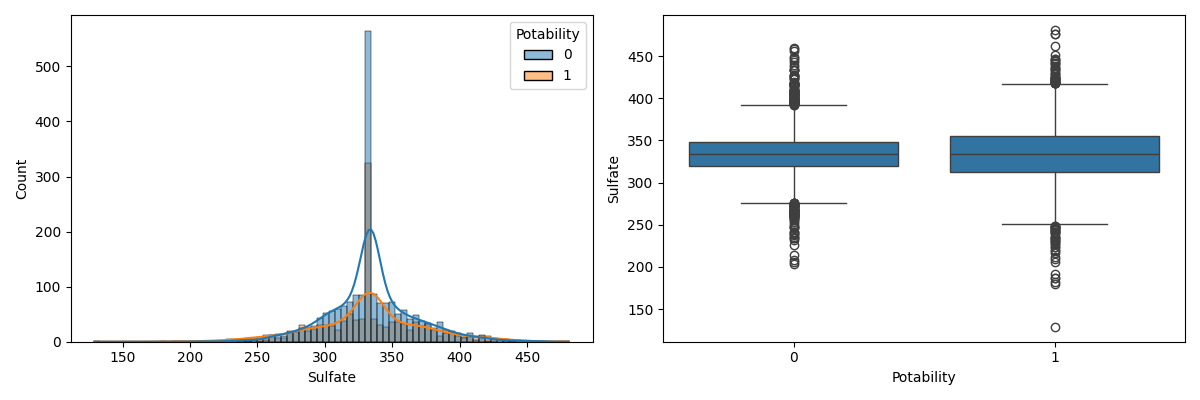
\includegraphics[width=0.9\textwidth]{IMAGE/dist_Sulfate.png}
    \caption{Phân phối của biến Sulfate sau tiền xử lý}
\end{figure}

\textbf{Nhận xét:} Giá trị Sulfate tập trung chủ yếu trong biên độ $[250-450]$ mg/L. Biểu đồ xác nhận việc điền khuyết $781$ dòng bằng giá trị $333.77$ đã được thực thi chính xác.

\paragraph{Biến "Hardness" (Độ cứng):} \leavevmode\\
\begin{figure}[H]
    \centering
    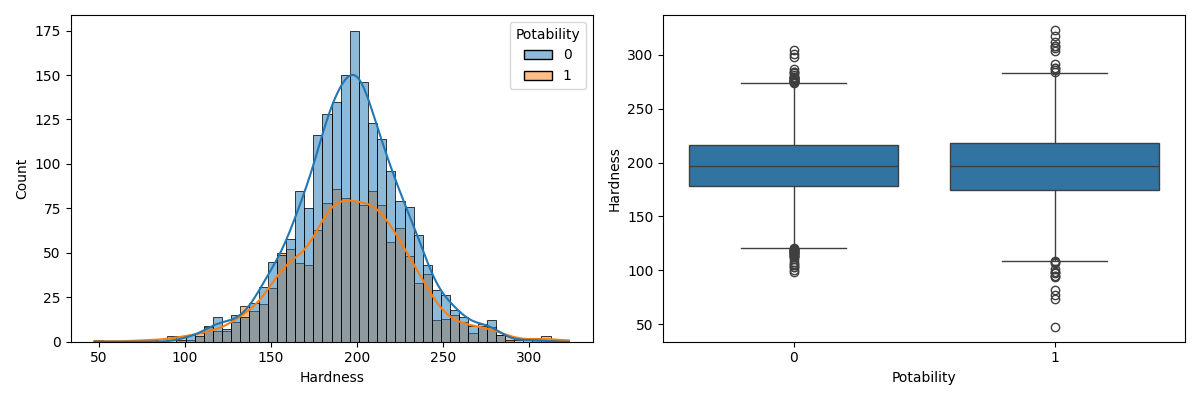
\includegraphics[width=0.9\textwidth]{IMAGE/dist_Hardness.png}
    \caption{Phân phối và biểu đồ hộp của biến Hardness}
\end{figure}
\textbf{Nhận xét:} Biểu đồ mang giá trị phân phối chuẩn ổn định trong biên độ $[100-250]$. Đây là cơ sở để nhóm thực hiện phân loại vào bảng \textbf{Dim\_Hardness}.

\paragraph{Biến "Solids" (Tổng chất rắn hòa tan):} \leavevmode\\
\begin{figure}[H]
    \centering
    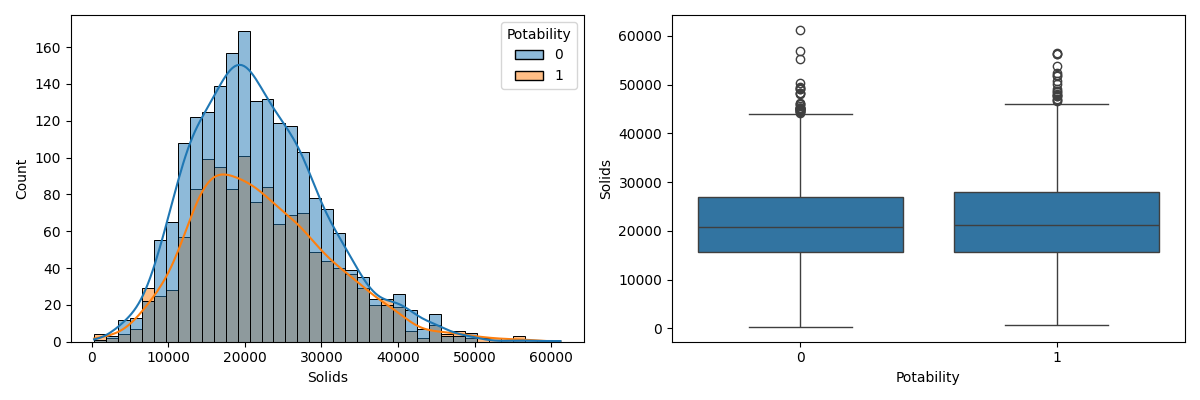
\includegraphics[width=0.9\textwidth]{IMAGE/dist_Solids.png}
    \caption{Phân phối và biểu đồ hộp của biến Solids}
\end{figure}

\textbf{Nhận xét:} Nồng độ Solids có phân phối lệch phải rõ rệt, tập trung trong khoảng $[15,000 - 30,000]$ ppm. Biểu đồ Boxplot xuất hiện nhiều giá trị ngoại lai vượt mức $50,000$ ppm.
\newpage
% ============================================================
% SECTION: QUY TRÌNH TÍCH HỢP ETL BẰNG PENTAHO
% Dự án: Kho Dữ Liệu Chất Lượng Nước (Water Potability)
% ============================================================

\section{Quy trình tích hợp ETL bằng Pentaho}

\subsection{Tổng quan kiến trúc hệ thống}

Hệ thống kho dữ liệu được xây dựng theo kiến trúc vi dịch vụ (microservices), triển khai hoàn toàn bằng Docker. Toàn bộ hệ thống bao gồm bốn thành phần chính được điều phối bởi \texttt{docker-compose}:

\begin{itemize}
    \item \textbf{PostgreSQL 15} (\texttt{dwh\_postgres}): Cơ sở dữ liệu mục tiêu lưu trữ kho dữ liệu, chạy trên cổng 5432.
    \item \textbf{Pentaho ETL Worker} (\texttt{dwh\_pentaho}): Container chạy Pentaho Data Integration phiên bản headless, thực thi file transformation \texttt{.ktr} thông qua công cụ dòng lệnh \texttt{pan.sh}.
    \item \textbf{Backend} (\texttt{dwh\_etl}): Container Python hỗ trợ phân tích và kết nối cơ sở dữ liệu thông qua SQLAlchemy.
    \item \textbf{Frontend} (\texttt{dwh\_frontend}): Giao diện web trực quan hóa kết quả phân tích.
\end{itemize}

Quá trình ETL được thực hiện bởi Pentaho Data Integration (PDI), phiên bản Community Edition, chạy không có giao diện đồ họa (headless mode) trong môi trường Docker với Java Runtime Environment phiên bản 17 (\texttt{eclipse-temurin:17-jre-alpine}).


\subsection{Thiết kế mô hình kho dữ liệu (Star Schema)}

Kho dữ liệu được thiết kế theo mô hình \textbf{Star Schema}, bao gồm một bảng sự kiện trung tâm và ba bảng chiều:

\subsubsection{Các bảng chiều (Dimension Tables)}

\begin{itemize}
    \item \textbf{\texttt{Dim\_Acidity}}: Phân loại độ axit của nước dựa trên giá trị pH.
    \begin{itemize}
        \item \textit{Axit}: pH $< 6.5$
        \item \textit{Trung tính}: $6.5 \leq$ pH $\leq 8.5$
        \item \textit{Kiềm}: pH $> 8.5$
    \end{itemize}

    \item \textbf{\texttt{Dim\_Hardness}}: Phân loại độ cứng của nước.
    \begin{itemize}
        \item \textit{Nước mềm}: Hardness $< 60$ mg/L
        \item \textit{Nước cứng vừa}: $60 \leq$ Hardness $< 120$ mg/L
        \item \textit{Nước cứng}: $120 \leq$ Hardness $< 180$ mg/L
        \item \textit{Nước rất cứng}: Hardness $\geq 180$ mg/L
    \end{itemize}

    \item \textbf{\texttt{Dim\_Potability}}: Phân loại khả năng uống của nước (0: Không an toàn, 1: An toàn).
\end{itemize}

\subsubsection{Bảng sự kiện (Fact Table)}

Bảng \textbf{\texttt{Fact\_Water\_Sample}} là bảng trung tâm lưu trữ toàn bộ các mẫu nước đã được xử lý, với khóa ngoại liên kết đến ba bảng chiều:

\begin{figure}[H]
\centering
\begin{tikzpicture}[
  scale=0.9, transform shape, % <--- Thu nhỏ 90% để không bị tràn lề
  every node/.style={font=\small},
  factbox/.style={draw, fill=blue!15, rounded corners=4pt,
                  minimum width=5.0cm, align=left, inner sep=6pt},
  dimbox/.style={draw, fill=orange!20, rounded corners=4pt,
                 minimum width=3.8cm, align=left, inner sep=6pt},
  fkarrow/.style={-{Latex[length=2.5mm]}, thick, dashed, gray}
]

% Fact table (center)
\node[factbox] (fact) {
  \textbf{Fact\_Water\_Sample}\\
  \rule{4.6cm}{0.4pt}\\
  \textbf{Water\_ID (PK, SERIAL)} \\
  ph\ DECIMAL(10,5)\\
  Hardness\ DECIMAL(10,5)\\
  Solids\ DECIMAL(15,5)\\
  Chloramines\ DECIMAL(10,5)\\
  Sulfate\ DECIMAL(10,5)\\
  Conductivity\ DECIMAL(10,5)\\
  Organic\_carbon\ DECIMAL(10,5)\\
  Trihalomethanes\ DECIMAL(10,5)\\
  Turbidity\ DECIMAL(10,5)\\
  \textit{Acidity\_Key}\ INT (FK)\\
  \textit{Hardness\_Key}\ INT (FK)\\
  \textit{Potability\_Key}\ INT (FK)
};

% Dim_Acidity (top-left) - Ép khoảng cách ngang còn 0.5cm
\node[dimbox, above left=1.8cm and 0.5cm of fact] (dimAcid) {
  \textbf{Dim\_Acidity}\\
  \rule{3.4cm}{0.4pt}\\
  \textbf{Acidity\_Key (PK)} \\
  Category\ VARCHAR(50)\\
  {\footnotesize (Axit / Trung tính / Kiềm)}
};

% Dim_Hardness (top-right) - Ép khoảng cách ngang còn 0.5cm
\node[dimbox, above right=1.8cm and 0.5cm of fact] (dimHard) {
  \textbf{Dim\_Hardness}\\
  \rule{3.4cm}{0.4pt}\\
  \textbf{Hardness\_Key (PK)} \\
  Category\ VARCHAR(50)\\
  {\footnotesize (Mềm/Vừa/Cứng/Rất cứng)}
};

% Dim_Potability (below)
\node[dimbox, below=1.8cm of fact] (dimPot) {
  \textbf{Dim\_Potability}\\
  \rule{3.4cm}{0.4pt}\\
  \textbf{Potability\_Key (PK)} \\
  Label\ VARCHAR(20)\\
  {\footnotesize (An toàn / Không an toàn)}
};

% FK arrows
\draw[fkarrow] (fact.north west) -- (dimAcid.south east)
  node[midway, sloped, above, font=\scriptsize] {Acidity\_Key};
\draw[fkarrow] (fact.north east) -- (dimHard.south west)
  node[midway, sloped, above, font=\scriptsize] {Hardness\_Key};
\draw[fkarrow] (fact.south) -- (dimPot.north)
  node[midway, right, font=\scriptsize] {Potability\_Key};

\end{tikzpicture}
\caption{Mô hình Star Schema của kho dữ liệu Water Potability}
\label{fig:star_schema}
\end{figure}

\subsection{Luồng xử lý ETL trong Pentaho (\texttt{water\_etl\_pipeline.ktr})}

File transformation \texttt{water\_etl\_pipeline.ktr} được thiết kế trực tiếp trong Pentaho Spoon và thực thi bằng công cụ \texttt{pan.sh}. Pipeline gồm \textbf{8 bước (steps)} được kết nối tuần tự theo luồng dữ liệu như sau:

% ---- TikZ ETL FLOWCHART ----
\begin{figure}[H]
\centering
\begin{tikzpicture}[
  scale=1.1, transform shape,
  every node/.style={font=\small},
  % Khối 1-7: Khóa cứng chiều ngang ở mức 6cm, đảm bảo tuyệt đối bằng nhau
  mainbox/.style={draw, fill=white, rounded corners=5pt,
                  minimum width=6cm, text width=5.8cm, minimum height=0.9cm,
                  align=center, inner sep=4pt},
  % Khối 8a, 8b: Thu nhỏ chiều ngang lại còn 4.5cm
  branchbox/.style={draw, fill=white, rounded corners=5pt,
                    minimum width=4.5cm, text width=4.3cm, minimum height=0.9cm,
                    align=center, inner sep=4pt},
  phaselbl/.style={font=\scriptsize\bfseries\itshape, text=gray!70, anchor=west},
  arr/.style={-{Latex[length=2.5mm]}, thick}
]

\def\sx{0}    % main column x
\def\lx{-3.5} % left branch x (đẩy nhẹ ra thêm để không dính nhau)
\def\rx{3.5}  % right branch x
\def\bracex{6.2} % tọa độ x của ngoặc nhọn
\def\lblx{6.4}   % tọa độ x của chữ chú thích

% --- CÁC KHỐI CHÍNH TỪ 1 ĐẾN 7 ---
\node[mainbox] (csv)  at (\sx, 0)     {\textbf{1.\ CSV file input}\\{\scriptsize \texttt{/data/raw/water\_potability.csv}, buf=50k}};
\node[mainbox] (null) at (\sx,-2.0)   {\textbf{2.\ If field value is null}\\{\scriptsize Điền mean: ph=7.08, Sulfate=333.77, THM=66.39}};
\node[mainbox] (nr1)  at (\sx,-4.0)   {\textbf{3.\ Number range (Hardness)}\\{\scriptsize $<$60 / 60--120 / 120--180 / $\geq$180 mg/L}};
\node[mainbox] (dh)   at (\sx,-6.0)   {\textbf{4.\ update dim\_hardness}\\{\scriptsize CombinationLookup, cache=9999, commit=100}};
\node[mainbox] (nr2)  at (\sx,-8.0)   {\textbf{5.\ Number range 2 (pH)}\\{\scriptsize $<$6.5 Axit / 6.5--8.5 Trung tính / $>$8.5 Kiềm}};
\node[mainbox] (da)   at (\sx,-10.0)  {\textbf{6.\ update dim\_acidity}\\{\scriptsize CombinationLookup, cache=9999, commit=100}};
\node[mainbox] (dp)   at (\sx,-12.0)  {\textbf{7.\ Dim\_potability lookup}\\{\scriptsize DBLookup trả về \texttt{fk\_potability}}};

% --- CÁC KHỐI NHÁNH ĐÃ ĐƯỢC THU NHỎ ---
\node[branchbox] (fact) at (\lx,-14.5)  {\textbf{8a.\ update fact}\\{\scriptsize TableOutput, batch=1000}};
\node[branchbox] (json) at (\rx,-14.5)  {\textbf{8b.\ JSON output}\\{\scriptsize \texttt{/data/eda\_results.json}}};

% --- VẼ MŨI TÊN ---
\draw[arr] (csv)  -- (null);
\draw[arr] (null) -- (nr1);
\draw[arr] (nr1)  -- (dh);
\draw[arr] (dh)   -- (nr2);
\draw[arr] (nr2)  -- (da);
\draw[arr] (da)   -- (dp);

% Rẽ nhánh mũi tên ở cuối
\draw[arr] (dp.south) -- ++(0,-0.8) -| (fact.north);
\draw[arr] (dp.south) -- ++(0,-0.8) -| (json.north);

% --- VẼ DẤU NGOẶC NHỌN ---
\draw[gray, thick, decorate, decoration={brace,amplitude=5pt}]
  (\bracex, 0.5) -- (\bracex,-0.5) node[midway]{};
\draw[gray, thick, decorate, decoration={brace,amplitude=5pt}]
  (\bracex,-1.5) -- (\bracex,-12.5) node[midway]{};
\draw[gray, thick, decorate, decoration={brace,amplitude=5pt}]
  (\bracex,-14.0) -- (\bracex,-15.0) node[midway]{};

% --- CHỮ CHÚ THÍCH CÁC GIAI ĐOẠN ---
\node[phaselbl] at (\lblx, 0)     {[E]xtract};
\node[phaselbl] at (\lblx,-7.0)   {[T]ransform};
\node[phaselbl] at (\lblx,-14.5)  {[L]oad};

\end{tikzpicture}
\caption{Sơ đồ luồng xử lý ETL trong Pentaho Transformation \texttt{water\_etl\_pipeline.ktr}}
\label{fig:etl_flow}
\end{figure}

\subsubsection{Bước 1: Đọc dữ liệu CSV (\texttt{CSV file input})}

Bước đầu tiên đọc dữ liệu thô từ file CSV tại đường dẫn \texttt{/data/raw/water\_potability.csv}. Các thông số cấu hình:
\begin{itemize}
    \item Dấu phân cách: dấu phẩy (\texttt{,})
    \item Ký tự bao quanh chuỗi: dấu nháy kép (\texttt{"})
    \item Dòng tiêu đề: có (header = Y)
    \item Kích thước bộ đệm: 50.000 bản ghi
    \item Toàn bộ 10 trường được khai báo kiểu \texttt{Number} hoặc \texttt{Integer} với độ chính xác cao
\end{itemize}

\subsubsection{Bước 2: Xử lý giá trị thiếu (\texttt{If field value is null})}

Bước này thực hiện \textbf{điền giá trị thay thế} cho các trường bị thiếu (NULL). Đây là bước tiền xử lý dữ liệu quan trọng, điền giá trị mặc định là giá trị trung bình (mean) của từng thuộc tính đã được tính từ bước EDA:

\begin{table}[H]
\centering
\caption{Giá trị điền thay thế cho các trường NULL}
\label{tab:null_replacement}
\begin{tabular}{lrl}
\hline
\textbf{Thuộc tính} & \textbf{Giá trị điền} & \textbf{Ghi chú} \\
\hline
\texttt{ph} & 7.08 & Trung bình pH \\
\texttt{Sulfate} & 333.77 & Trung bình Sulfate (mg/L) \\
\texttt{Trihalomethanes} & 66.39 & Trung bình Trihalomethanes ($\mu$g/L) \\
\hline
\end{tabular}
\end{table}

Chỉ có ba thuộc tính chứa giá trị NULL trong bộ dữ liệu; các thuộc tính còn lại đã đầy đủ.

\subsubsection{Bước 3: Phân loại độ cứng (\texttt{Number range})}

Sử dụng bước \textbf{Number Range} để ánh xạ giá trị số \texttt{Hardness} thành nhãn phân loại \texttt{Hardness\_Category} theo các ngưỡng chuẩn quốc tế:

\begin{table}[H]
\centering
\caption{Quy tắc phân loại độ cứng}
\label{tab:hardness_range}
\begin{tabular}{lcc}
\hline
\textbf{Danh mục} & \textbf{Giới hạn dưới (mg/L)} & \textbf{Giới hạn trên (mg/L)} \\
\hline
Nước mềm & $-\infty$ & $< 60$ \\
Nước cứng vừa & $\geq 60$ & $< 120$ \\
Nước cứng & $\geq 120$ & $< 180$ \\
Nước rất cứng & $\geq 180$ & $+\infty$ \\
\hline
\end{tabular}
\end{table}

\subsubsection{Bước 4: Cập nhật chiều độ cứng (\texttt{update dim\_hardness})}

Sử dụng bước \textbf{Combination Lookup/Update} để tra cứu khóa chiều \texttt{hardness\_key} từ bảng \texttt{dim\_hardness} dựa trên \texttt{Hardness\_Category}. Nếu giá trị chưa tồn tại, bước này sẽ tự động tạo bản ghi mới (insert). Cơ chế:
\begin{itemize}
    \item Trường tra cứu: \texttt{Hardness\_Category} $\rightarrow$ cột \texttt{category} trong DB
    \item Khóa trả về: \texttt{hardness\_key} (sử dụng phương thức \texttt{tablemax} để tự tăng)
    \item Kích thước cache: 9.999 bản ghi; kích thước batch commit: 100
\end{itemize}

\subsubsection{Bước 5: Phân loại độ axit (\texttt{Number range 2})}

Tương tự bước 3, bước này ánh xạ giá trị \texttt{ph} thành nhãn \texttt{Acidity\_Category} dựa trên thang pH tiêu chuẩn:

\begin{table}[H]
\centering
\caption{Quy tắc phân loại độ axit}
\label{tab:acidity_range}
\begin{tabular}{lcc}
\hline
\textbf{Danh mục} & \textbf{Giới hạn dưới} & \textbf{Giới hạn trên} \\
\hline
Axit & $-\infty$ & $< 6.5$ \\
Trung tính & $\geq 6.5$ & $\leq 8.5$ \\
Kiềm & $> 8.5$ & $+\infty$ \\
\hline
\end{tabular}
\end{table}

\subsubsection{Bước 6: Cập nhật chiều độ axit (\texttt{update dim\_acidity})}

Hoạt động theo cơ chế giống bước 4, tra cứu và cập nhật bảng \texttt{dim\_acidity} dựa trên \texttt{Acidity\_Category}, trả về \texttt{acidity\_key}.

\subsubsection{Bước 7: Tra cứu chiều khả năng uống (\texttt{Dim\_potability lookup})}

Sử dụng bước \textbf{Database Lookup} để tra cứu \texttt{potability\_key} từ bảng \texttt{dim\_potability} dựa trên giá trị \texttt{Potability} (0 hoặc 1) từ dữ liệu gốc. Giá trị trả về được đặt tên \texttt{fk\_potability} để phân biệt với trường gốc.

Sau bước này, mỗi bản ghi dữ liệu đã có đầy đủ ba khóa ngoại:
\begin{itemize}
    \item \texttt{hardness\_key} $\rightarrow$ \texttt{Dim\_Hardness}
    \item \texttt{acidity\_key} $\rightarrow$ \texttt{Dim\_Acidity}
    \item \texttt{fk\_potability} $\rightarrow$ \texttt{Dim\_Potability}
\end{itemize}

\subsubsection{Bước 8a: Nạp vào bảng sự kiện (\texttt{update fact})}

Bước \textbf{Table Output} thực hiện \textbf{Load} dữ liệu vào bảng \texttt{fact\_water\_sample}. Cấu hình:
\begin{itemize}
    \item Kích thước batch commit: 1.000 bản ghi (tối ưu hiệu suất)
    \item Chế độ batch insert: bật (\texttt{use\_batch = Y})
    \item Chỉ định rõ ánh xạ cột: bật (\texttt{specify\_fields = Y})
    \item Không truncate bảng trước khi nạp (cho phép chạy lại tăng dần)
\end{itemize}

Ánh xạ trường từ luồng dữ liệu sang cột trong DB:

\begin{table}[H]
\centering
\caption{Ánh xạ trường khi nạp vào Fact Table}
\label{tab:fact_mapping}
\begin{tabular}{ll}
\hline
\textbf{Trường trong luồng dữ liệu} & \textbf{Cột trong \texttt{fact\_water\_sample}} \\
\hline
\texttt{ph} & \texttt{ph} \\
\texttt{Hardness} & \texttt{hardness} \\
\texttt{Solids} & \texttt{solids} \\
\texttt{Chloramines} & \texttt{chloramines} \\
\texttt{Sulfate} & \texttt{sulfate} \\
\texttt{Conductivity} & \texttt{conductivity} \\
\texttt{Organic\_carbon} & \texttt{organic\_carbon} \\
\texttt{Trihalomethanes} & \texttt{trihalomethanes} \\
\texttt{Turbidity} & \texttt{turbidity} \\
\texttt{hardness\_key} & \texttt{hardness\_key} \\
\texttt{acidity\_key} & \texttt{acidity\_key} \\
\texttt{fk\_potability} & \texttt{potability\_key} \\
\hline
\end{tabular}
\end{table}

\subsubsection{Bước 8b: Xuất kết quả JSON (\texttt{JSON output})}

Song song với việc nạp vào CSDL, luồng dữ liệu được rẽ nhánh để xuất ra file \texttt{/data/eda\_results.json}. File JSON này phục vụ trực tiếp cho Frontend để hiển thị kết quả phân tích mà không cần truy vấn lại CSDL. Các trường được xuất bao gồm toàn bộ thuộc tính gốc cộng với các nhãn phân loại và khóa chiều được sinh ra trong quá trình ETL.

\subsection{Kết nối cơ sở dữ liệu}

Pentaho kết nối đến PostgreSQL thông qua kết nối JDBC được cấu hình trong file \texttt{water\_etl\_pipeline.ktr}:
 
\begin{table}[H]
\centering
\caption{Thông số kết nối CSDL trong Pentaho}
\label{tab:db_conn}
\begin{tabular}{ll}
\hline
\textbf{Tham số} & \textbf{Giá trị} \\
\hline
\texttt{name} & \texttt{data\_warehouse} \\
\texttt{type} & PostgreSQL (Native/JDBC) \\
\texttt{server} & \texttt{db} \\
\texttt{port} & $5432$ \\
\texttt{username} & \texttt{admin} \\
\hline
\end{tabular}
\end{table}

Trong môi trường Docker, tên máy chủ \texttt{db} được Docker DNS tự động phân giải thành địa chỉ IP nội bộ của container PostgreSQL nhờ cơ chế Docker Compose network.

\subsection{Triển khai và thực thi}

\subsubsection{Đóng gói mã nguồn bằng Docker}

Container Pentaho được xây dựng dựa trên image \texttt{eclipse-temurin:17-jre-alpine}, một Java Runtime Environment nhẹ phù hợp cho môi trường triển khai. Quá trình khởi động được điều khiển bởi script \texttt{start\_pentaho.sh}:
\begin{lstlisting}
    export JAVA_HOME=/opt/java/openjdk
    export PENTAHO_JAVA_HOME=$JAVA_HOME
    export PATH=$JAVA_HOME/bin:$PATH
    
    PDI_DIR="/app/data-integration"
    
    if [ ! -d "$JAVA_HOME" ]; then
        echo "Error: Java directory not found at $JAVA_HOME"
        exit 1
    fi
    
    if [ ! -d "$PDI_DIR" ]; then
        echo "Error: Pentaho directory not found at $PDI_DIR"
        echo "Hệ thống đang tìm tại: $PDI_DIR"
        echo "Hãy đảm bảo thư mục 'data-integration' nằm trong folder 'pentaho/' của dự án."
        exit 1
    fi
    
    echo "Đang khởi động Pentaho ETL..."
    cd "$PDI_DIR"
    chmod +x /app/data-integration/*.sh
    /app/data-integration/pan.sh -file="/etl/water_etl_pipeline.ktr" -level=Basic
\end{lstlisting}

\begin{enumerate}
    \item Kiểm tra sự tồn tại của \texttt{JAVA\_HOME} và thư mục PDI
    \item Cấp quyền thực thi cho tất cả file \texttt{.sh} trong thư mục Pentaho
    \item Gọi lệnh: \verb|pan.sh -file="/etl/water_etl_pipeline.ktr" -level=Basic|
\end{enumerate}

Thư mục \texttt{/etl} (chứa file \texttt{.ktr}) và \texttt{/data} (chứa dữ liệu CSV đầu vào và JSON đầu ra) được mount từ máy chủ vào container thông qua Docker volumes, đảm bảo tính bền vững của dữ liệu giữa các lần chạy.

% \subsubsection{Khởi tạo lược đồ tự động}

% Khi PostgreSQL container khởi động, script \texttt{01\_schema.sql} trong thư mục \texttt{/docker-entrypoint-initdb.d/} được PostgreSQL tự động thực thi, tạo toàn bộ bảng chiều, bảng sự kiện, và dữ liệu ban đầu (seed data) cho các bảng chiều tĩnh.

\subsection{Tóm tắt quy trình ETL}

\begin{table}[H]
\centering
\caption{Tóm tắt các giai đoạn ETL}
\label{tab:etl_summary}
\begin{tabular}{llp{7cm}}
\hline
\textbf{Giai đoạn} & \textbf{Công cụ/Bước} & \textbf{Nội dung xử lý} \\
\hline
\textbf{Extract} & \text{CSV file input} & Đọc dữ liệu thô \\
\hline
\multirow{4}{*}{\textbf{Transform}} & \text{If field value is null} & Điền trung bình vào 3 trường bị thiếu \\
 & \text{Number range} & Phân loại Hardness $\rightarrow$ 4 nhóm độ cứng \\
 & \text{Number range 2} & Phân loại pH $\rightarrow$ 3 nhóm độ axit \\
 & \text{Dim lookup} & Tra cứu khóa ngoại từ 3 bảng chiều \\
\hline
\multirow{2}{*}{\textbf{Load}} & \text{update fact} & Nạp vào \texttt{fact\_water\_sample} (batch 1.000) \\
 & \texttt{JSON} output & Xuất file JSON cho Frontend \\
\hline
\end{tabular}
\end{table}

Quy trình ETL được thiết kế theo nguyên tắc \textbf{idempotency} (có thể chạy lại mà không gây lỗi nhân đôi dữ liệu trong bảng chiều) nhờ cơ chế \texttt{Combination Lookup/Update} của Pentaho, cho phép chỉ insert bản ghi mới nếu chưa tồn tại, ngược lại trả về khóa đã có.

% ============================================================
\subsection{Đánh giá hiệu năng và chất lượng quy trình ETL}
% ============================================================

\subsubsection{Cấu hình hiệu năng}

Pipeline được cấu hình với các tham số tối ưu hiệu năng trực tiếp trong file \texttt{.ktr}:

\begin{table}[H]
\centering
\caption{Các tham số hiệu năng của Pentaho Transformation}
\label{tab:perf_params}
\begin{tabular}{lrp{6cm}}
\hline
\textbf{Tham số} & \textbf{Giá trị} & \textbf{Tác dụng} \\
\hline
\texttt{size\_rowset} & 10.000 & Dung lượng hàng đợi giữa các step \\
\texttt{sleep\_time\_empty} & 50 ms & Thời gian chờ khi buffer rỗng \\
\texttt{sleep\_time\_full} & 50 ms & Thời gian chờ khi buffer đầy \\
\texttt{feedback\_size} & 50.000 & Ngưỡng hiển thị tiến trình xử lý \\
\texttt{buffer\_size} (CSV) & 50.000 & Số bản ghi đọc trước vào bộ nhớ \\
Batch commit (Dim) & 100 & Số bản ghi/lần commit cho bảng chiều \\
Batch commit (Fact) & 1.000 & Số bản ghi/lần commit cho bảng sự kiện \\
Dim cache size & 9.999 & Số bản ghi cache tránh truy vấn CSDL \\
\hline
\end{tabular}
\end{table}

Việc sử dụng \textbf{batch insert} với kích thước 1.000 bản ghi cho bảng fact giúp giảm đáng kể số lần round-trip đến PostgreSQL so với insert từng dòng. Cache kích thước 9.999 cho các bảng chiều gần như loại bỏ hoàn toàn các truy vấn lookup lặp lại, vì bộ dữ liệu Water Potability chỉ có 3--4 giá trị phân loại duy nhất cho mỗi chiều.

\subsubsection{Phân tích chất lượng dữ liệu sau ETL}

Dựa trên kết quả từ bước EDA (phân tích khám phá dữ liệu) và cấu hình xử lý NULL trong pipeline, chất lượng dữ liệu sau ETL được đánh giá như sau:

\begin{table}[H]
\centering
\caption{Tổng kết chất lượng dữ liệu trước và sau ETL}
\label{tab:data_quality}
\begin{tabular}{lccl}
\hline
\textbf{Thuộc tính} & \textbf{\% NULL (trước)} & \textbf{\% NULL (sau)} & \textbf{Phương pháp xử lý} \\
\hline
\texttt{ph} & $\sim$14.98\% & 0\% & Điền mean (7.08) \\
\texttt{Sulfate} & $\sim$23.84\% & 0\% & Điền mean (333.77 mg/L) \\
\texttt{Trihalomethanes} & $\sim$4.93\% & 0\% & Điền mean (66.39 $\mu$g/L) \\
Các thuộc tính khác & 0\% & 0\% & Không cần xử lý \\
\hline
\end{tabular}
\end{table}

Việc điền giá trị trung bình (mean imputation) là lựa chọn phù hợp vì:
\begin{itemize}
    \item Phân phối của các thuộc tính xấp xỉ phân phối chuẩn (đã xác nhận qua EDA).
    \item Giá trị mean không tạo ra các giá trị ngoại lệ (outlier) mới.
    \item Đảm bảo tính toàn vẹn referential integrity khi nạp vào bảng fact.
\end{itemize}

\subsubsection{Tính đúng đắn của phân loại chiều}

Hai bảng chiều \texttt{Dim\_Acidity} và \texttt{Dim\_Hardness} sử dụng các ngưỡng phân loại dựa trên tiêu chuẩn quốc tế:

\begin{itemize}
    \item \textbf{Độ pH}: Ngưỡng 6.5 và 8.5 tuân theo tiêu chuẩn WHO (World Health Organization) về chất lượng nước uống - nước an toàn có pH trong khoảng 6.5--8.5.
    \item \textbf{Độ cứng}: Các ngưỡng $<$60, $60-120$, $120-180$ và $\geq180 mg/L$ (CaCO$_3$) tương ứng với phân loại nước mềm, cứng vừa, cứng và rất cứng theo thang phân loại của USGS (United States Geological Survey).
\end{itemize}

\subsection{Nhận xét tổng thể}

Quy trình ETL triển khai bằng Pentaho Data Integration đã đáp ứng đầy đủ các yêu cầu của một pipeline kho dữ liệu chuyên nghiệp:

\begin{enumerate}
    \item \textbf{Tính đầy đủ (Completeness)}: Toàn bộ 3.276 mẫu nước được nạp vào kho dữ liệu sau khi xử lý giá trị thiếu.
    \item \textbf{Tính nhất quán (Consistency)}: Khóa chiều được sinh ra nhất quán thông qua cơ chế \texttt{Combination Lookup/Update}, tránh trùng lặp trong bảng chiều.
    \item \textbf{Tính lũy đẳng (Idempotency)}: Pipeline có thể chạy lại nhiều lần mà không gây lỗi nhờ cơ chế lookup-before-insert.
    \item \textbf{Khả năng truy vấn (Queryability)}: Mô hình Star Schema cho phép các câu truy vấn phân tích đa chiều hiệu quả, ví dụ: thống kê tỉ lệ nước an toàn theo nhóm độ cứng hoặc độ axit.
    \item \textbf{Khả năng mở rộng (Scalability)}: Kiến trúc Docker + batch processing cho phép mở rộng khi kích thước dữ liệu tăng mà không cần thay đổi logic ETL.
\end{enumerate}

Hạn chế chính của quy trình hiện tại là chưa có cơ chế \textbf{incremental load} thực sự (chỉ kiểm tra bảng chiều, không kiểm tra bảng fact), do đó nếu chạy lại pipeline trên cùng bộ dữ liệu sẽ tạo ra các bản ghi trùng lặp trong \texttt{fact\_water\_sample}. Trong tương lai, có thể bổ sung bước kiểm tra trùng lặp hoặc sử dụng chiến lược \textit{upsert} cho bảng fact.

\newpage
\section{Xây dựng mô hình dự đoán}

\subsection{Tiền xử lý và chia tập huấn luyện}
\hspace{17pt}Trước khi đưa dữ liệu vào huấn luyện các mô hình học máy, một bước đánh giá cực kỳ quan trọng là phải kiểm chứng xem tập dữ liệu kiểm thử (Test set - 20\%) có mang tính đại diện chính xác cho tập dữ liệu huấn luyện (Train set - 80\%) hay không. Nếu phân phối của hai tập này bị lệch (Data Drift), kết quả đánh giá mô hình sẽ không còn phản ánh đúng năng lực dự đoán thực tế.

\hspace{17pt}Đầu tiên, nhóm tiến hành kiểm tra sự phân bổ của biến mục tiêu (\texttt{Potability}) ở cả hai tập:
\begin{figure}[H]
    \centering
    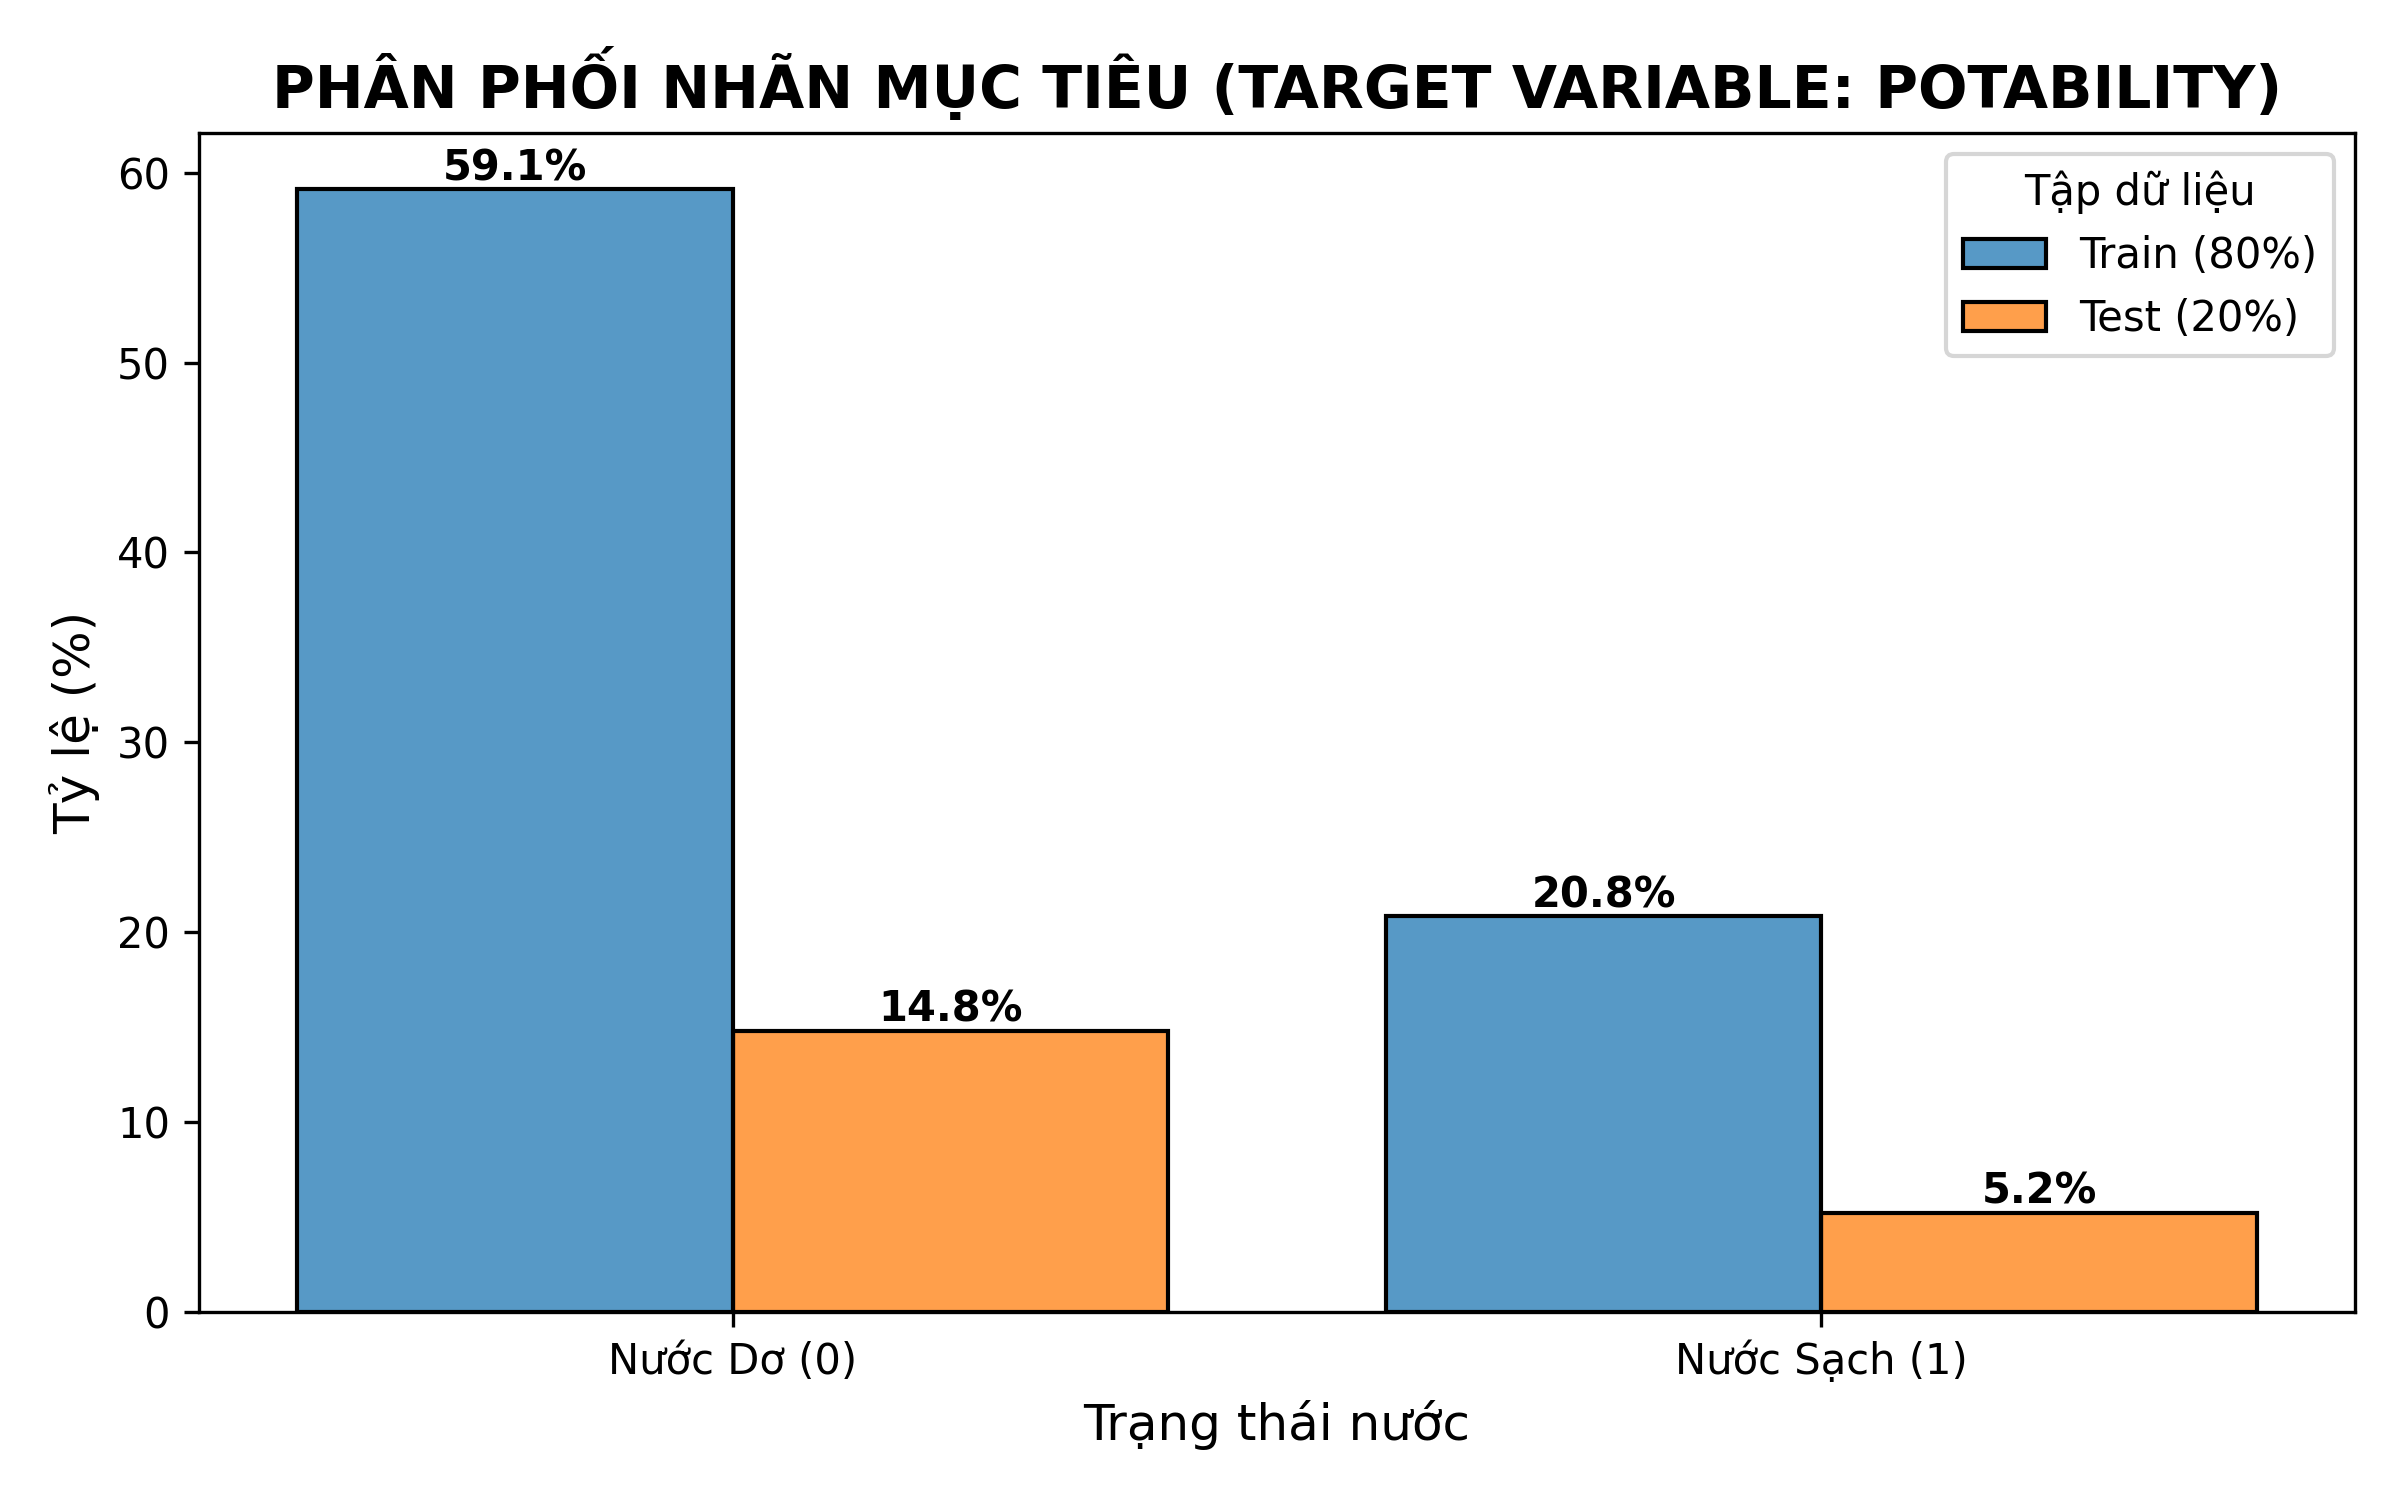
\includegraphics[width=1.0\linewidth]{IMAGE-MODELS/Histogram_Target_Plot.png}
    \caption{
    Phân phối nhãn mục tiêu (Potability) trên tập Train và Test}
    \label{fig:placeholder}
\end{figure}

\hspace{17pt}Tiếp theo, nhóm tiến hành kiểm tra cấu trúc phân phối của toàn bộ các đặc trưng hóa lý (Features) đầu vào:
\begin{figure}[H]
    \centering
    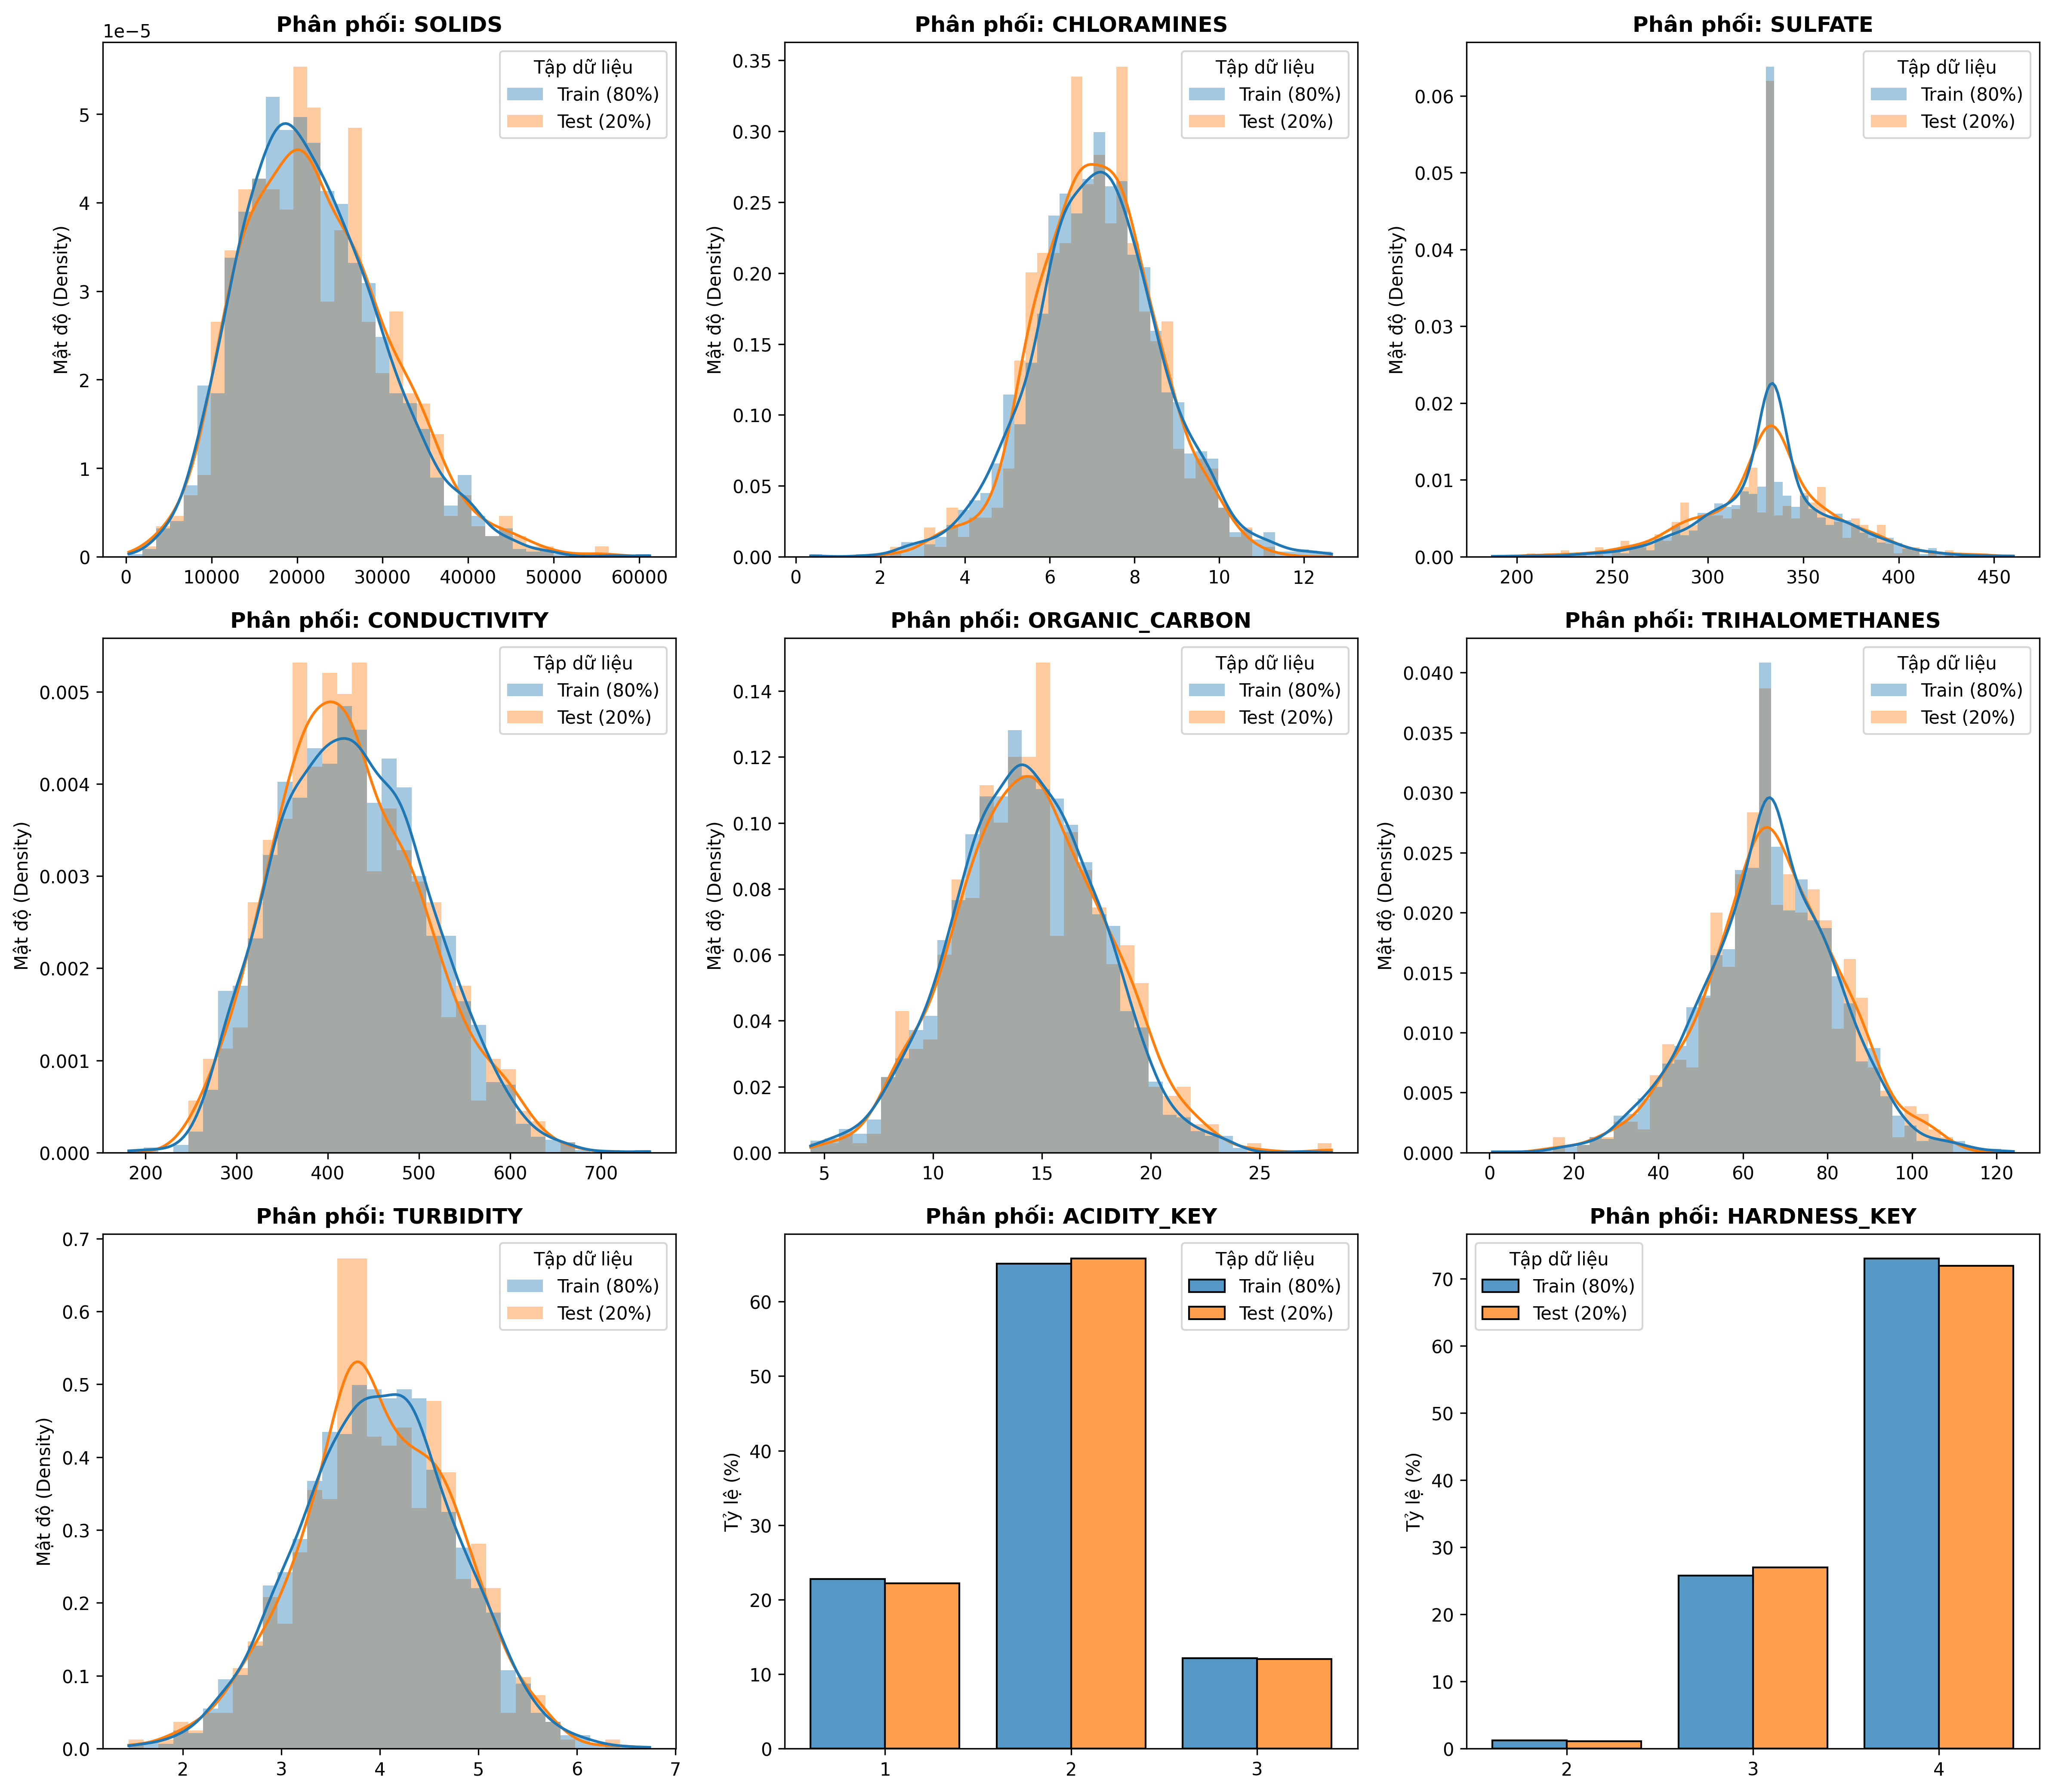
\includegraphics[width=1.0\linewidth]{IMAGE-MODELS/Histogram_Features_Plot.png}
    \caption{So sánh phân phối của các đặc trưng hóa lý trên tập Train và Test}
    \label{fig:features_dist}
\end{figure}
\hspace{17pt}Biểu đồ Hình \ref{fig:features_dist} cung cấp cái nhìn tổng quan về mật độ phân phối của các đặc trưng:
\begin{itemize}
    \item \textbf{Sự đồng nhất về phân phối:} Đường cong mật độ (KDE) của tập Train (màu xanh) và tập Test (màu cam) gần như chồng khít lên nhau ở tất cả các biến liên tục như \texttt{Solids}, \texttt{Chloramines}, hay \texttt{Conductivity}. Các biến rời rạc (\texttt{Acidity\_key}, \texttt{Hardness\_key}) cũng bảo toàn hoàn toàn cấu trúc tỷ lệ. Điều này khẳng định tập Test chứa các mẫu ngẫu nhiên và mang tính đại diện cực kỳ tốt cho tập Train.
    \item \textbf{Dấu vết của quá trình ETL (Imputation Artifact):} Điểm đáng chú ý là đỉnh nhọn bất thường xuyên thủng đường phân phối chuẩn tại biểu đồ \texttt{Sulfate} và \texttt{Trihalomethanes}. Đây không phải là lỗi dữ liệu, mà chính là minh chứng trực quan cho bước ETL Điền khuyết (Imputation) bằng giá trị trung bình/trung vị đã thực hiện ở giai đoạn trước đối với các giá trị \texttt{NaN}. Mặc dù tạo ra đỉnh nhọn, nhưng đỉnh này xuất hiện đồng đều ở cả tập Train và Test, đảm bảo tính nhất quán của dữ liệu.
\end{itemize}

\hspace{17pt}Với nền tảng dữ liệu đã được làm sạch, chuẩn hóa và phân tách đồng nhất, hệ thống đã hoàn toàn sẵn sàng cho quá trình huấn luyện và tối ưu siêu tham số các mô hình học máy.
Quá trình tiền xử lý đóng vai trò quyết định trong việc loại bỏ nhiễu và nâng cao chất lượng dữ liệu trước khi đưa vào mô hình học máy. Dữ liệu đầu vào được trích xuất trực tiếp từ kho dữ liệu (bảng \textit{fact\_water\_sample}) và đi qua các bước xử lý sau:

\begin{itemize}
    \item \textbf{Lựa chọn đặc trưng:} Lựa chọn các biến độc lập quan trọng bao gồm: \textit{solids, chloramines, sulfate, conductivity, organic\_carbon, trihalomethanes, turbidity}. Riêng hai đặc trưng \textit{pH} và \textit{hardness} được sử dụng dưới dạng đã được rời rạc hóa (binning) thành \textit{acidity\_key} và \textit{hardness\_key} để tối ưu khả năng phân loại của mô hình.
    
    \item \textbf{Làm sạch dữ liệu theo logic thực tế:} Nhằm loại bỏ các điểm dữ liệu phi thực tế. Dù có nhãn uống được (\textit{$Portability = 1$}), nhưng các chỉ số hóa lý lại ở mức độc hại. Các điều kiện lọc sau được áp dụng để xóa bỏ các bản ghi lỗi:
    \begin{itemize}
        \item Nước có tính axit mạnh ($pH<6.5$) hoặc kiềm mạnh ($pH> 8.5$).
        \item Nồng độ Sulfate vượt ngưỡng an toàn ($>400$).
        \item Tổng chất rắn hòa tan (Solids) quá cao ($>40000$), biểu hiện của nước quá mặn hoặc bị ô nhiễm nghiêm trọng.
        \item Độ đục (Turbidity) ở mức ngầu bùn ($>7$).
    \end{itemize}
    
    \item \textbf{Chia tập dữ liệu huấn luyện và kiểm thử:} Dữ liệu sau khi làm sạch được chia thành tập huấn luyện (80\%) và tập kiểm thử (20\%). Kỹ thuật phân tầng (\textit{stratify}) được áp dụng dựa trên nhãn mục tiêu nhằm đảm bảo tỷ lệ phân bố giữa lớp an toàn và không an toàn được giữ nguyên ở cả hai tập, hạn chế tối đa sự mất cân bằng lớp.
    
    \item \textbf{Chuẩn hóa dữ liệu (Data Scaling):} Sử dụng \textit{StandardScaler} để đưa các đặc trưng về cùng một dải phân phối chuẩn (trung bình bằng 0 và phương sai bằng 1). Quá trình fit\_transform được thực hiện trên tập huấn luyện và sau đó transform trên tập kiểm thử. Việc chuẩn hóa này là yêu cầu bắt buộc để các thuật toán dựa trên khoảng cách (như SVM) không bị sai lệch bởi sự chênh lệch đơn vị đo.
\end{itemize}

\subsection{Phương thức đánh giá mô hình}
Để đánh giá hiệu suất của các mô hình phân lớp một cách toàn diện, thay vì chỉ dựa vào độ chính xác (Accuracy), nghiên cứu tập trung vào việc đánh giá khả năng nhận diện đúng mẫu nước an toàn (Lớp 1). Các độ đo chính được sử dụng bao gồm: Precision (Độ chính xác dự đoán), Recall (Độ bao phủ) và F1-Score (Trung bình điều hòa giữa Precision và Recall).

Một điểm đáng chú ý trong phương pháp đánh giá của nghiên cứu này là kỹ thuật \textbf{Quét ngưỡng quyết định (Threshold Scanning)}. Thay vì sử dụng ngưỡng mặc định là 0.5 để phân lớp, hệ thống thực hiện quét liên tục các ngưỡng xác suất (từ 0.5 đến 0.8 với bước nhảy 0.02) dựa trên kết quả \textit{predict\_proba}. Kỹ thuật này giúp tìm ra ngưỡng cắt tối ưu nhất, cho phép cân bằng linh hoạt giữa việc không bỏ sót nguồn nước an toàn (Recall cao) và đảm bảo không uống nhầm nước độc hại (Precision cao). 

Quá trình hiện thực kỹ thuật quét ngưỡng được thể hiện chi tiết trong Đoạn mã \ref{lst:threshold_scanning}.

\begin{lstlisting}[language=Python, caption={Thuật toán quét ngưỡng quyết định (Threshold Scanning)}, label={lst:threshold_scanning}]
thresholds = np.arange(0.5, 0.8, 0.02)
for name, model in models.items():
    test_data = X_test_scaled if name == "SVM" else X_test
    y_proba = model.predict_proba(test_data)[:, 1]
    for th in thresholds:
        th = round(th, 2)
        y_pred_custom = (y_proba >= th).astype(int)
        
        report = classification_report(y_test, y_pred_custom, 
                                       output_dict=True, zero_division=0)
        
        p1 = report['1']['precision']
        r1 = report['1']['recall']
        f1 = report['1']['f1-score']
        acc = report['accuracy']
\end{lstlisting}
\subsection{Hiện thực mô hình dự đoán}
Nghiên cứu tiến hành cài đặt và huấn luyện ba thuật toán học máy phổ biến và mạnh mẽ nhất cho bài toán phân lớp:
\begin{enumerate}
    \item \textbf{Random Forest:} Thuật toán học tập hợp (Ensemble Learning) dựa trên cây quyết định, được thiết lập với 100 cây ước lượng (\textit{n\_estimators=100}). Thuật toán này có khả năng tự xử lý tốt các đặc trưng phi tuyến và không yêu cầu khắt khe về việc chuẩn hóa dữ liệu.
    \item \textbf{XGBoost (Extreme Gradient Boosting):} Mô hình Boosting mạnh mẽ với 100 bộ ước lượng, giúp tối ưu hóa hàm mất mát thông qua việc học tuần tự từ các sai số của các cây quyết định trước đó.
    \item \textbf{Support Vector Machine (SVM):} Được cấu hình với hàm nhân phi tuyến RBF (\textit{kernel='rbf'}) để xử lý không gian dữ liệu phức tạp và bật tính năng tính toán xác suất (\textit{probability=True}) phục vụ cho bước quét ngưỡng. Mô hình này được huấn luyện trực tiếp trên tập dữ liệu đã qua chuẩn hóa (\textit{X\_train\_scaled}).
\end{enumerate}

Thay vì sử dụng các tham số mặc định của thư viện, nghiên cứu áp dụng kỹ thuật \texttt{RandomizedSearchCV} với kiểm chứng chéo 5 nếp gấp (5-fold CV) để tự động dò tìm tổ hợp siêu tham số tối ưu nhất cho Random Forest và XGBoost. Riêng mô hình SVM được thiết lập cấu hình tĩnh do đặc thù thuật toán đòi hỏi chi phí tính toán phần cứng quá lớn.

\hspace{17pt}Để thực hiện việc dò tìm, nhóm đã định nghĩa một không gian siêu tham số (Hyperparameter Grid) bao gồm các tổ hợp giá trị tiềm năng nhất, kết hợp với danh sách các đặc trưng đầu vào và dải ngưỡng quét (Threshold Sweep). Toàn bộ được cấu hình tập trung và quản lý độc lập như sau:

\begin{lstlisting}[language=Python, caption=Cấu hình đặc trưng và không gian siêu tham số cho các mô hình]
import numpy as np

# 1. Cau hinh Data (Features)
FEATURES_TO_USE = [
    'solids', 'chloramines', 'sulfate', 'conductivity',
    'organic_carbon', 'trihalomethanes', 'turbidity',
    'acidity_key', 'hardness_key'  
]

# 2. Khong gian Sieu tham so (Hyperparameter Grids)
RF_PARAMS = {
    'n_estimators': [100, 200, 300, 500],
    'max_depth': [None, 10, 20, 30], # Do sau toi da cua cay
    'min_samples_split': [2, 5, 10], # So mau toi thieu de tach nhanh
    'random_state': [42],
    'class_weight': [None, 'balanced'] 
}

XGB_PARAMS = {
    'n_estimators': [100, 200, 300],
    'learning_rate': [0.01, 0.1, 0.2],
    'max_depth': [3, 5, 7],
    'subsample': [0.8, 1.0]
}

# Tham so tinh cho SVM
SVM_PARAMS = {
    'kernel': 'rbf',
    'probability': True,
    'random_state': 42
}

THRESHOLDS_SWEEP = np.arange(0.5, 0.8, 0.05) 
\end{lstlisting}
Sau khi các mô hình hoàn tất quá trình huấn luyện và quét ngưỡng để đối chiếu hiệu suất, các mô hình đạt kết quả tốt nhất (bao gồm Random Forest và SVM) cùng với bộ chuẩn hóa dữ liệu (Scaler) được đóng gói và xuất ra dưới định dạng tệp \textit{.pkl} thông qua thư viện \textit{joblib}. Việc xuất tệp này giúp lưu trữ lại trạng thái đã học của hệ thống, sẵn sàng cho việc tích hợp, triển khai vào các ứng dụng thực tế hoặc API dự đoán về sau mà không cần phải huấn luyện lại từ đầu.
\subsection{Kết quả thực nghiệm và phân tích mô hình}
Sau quá trình huấn luyện và dò tìm siêu tham số tối ưu (Hyperparameter Tuning), các mô hình được đưa vào đánh giá trên tập dữ liệu kiểm thử (Test set). Báo cáo trích xuất kết quả dự đoán với ngưỡng quyết định mặc định (Threshold = $0.5$) để tiến hành so sánh cấu trúc Confusion Matrix (Confusion Matrix) và các chỉ số đo lường hiệu suất.

\subsubsection{Giải thuật Rừng ngẫu nhiên (Random Forest)}
\begin{table}[H]
    \centering
    \renewcommand{\arraystretch}{1.2}
    \begin{tabular}{ccccc}
        \hline
        \textbf{Threshold} & \textbf{Precision} & \textbf{Recall} & \textbf{F1-Score} & \textbf{Accuracy} \\
        \hline
        \color{red}0.50 & \color{red}0.5520 &\color{red} 0.2979 &\color{red} 0.3871 &\color{red} 0.7542 \\

        0.55 & 0.5818 & 0.2087 & 0.3083 & 0.7568 \\
  
        0.60 & 0.5652 & 0.0822 & 0.1585 & 0.7449 \\

        0.65 & 0.8333 & 0.0730 & 0.1387 & 0.7542 \\

        0.70 & 1.0000 & 0.0426 & 0.0816 & 0.7505 \\

        0.75 & 1.0000 & 0.0426 & 0.0816 & 0.7505 \\

        0.80 & 1.0000 & 0.0335 & 0.0645 & 0.7486 \\
        \hline
    \end{tabular}
    \caption{Kết quả đo lường hiệu suất của mô hình Random Forest qua các ngưỡng}
    \label{tab:rf_metrics}
\end{table}
Thông qua quá trình quét ngẫu nhiên 
`RandomizedSearchCV`, bộ siêu tham số tối ưu nhất được tìm thấy cho Random Forest bao gồm: \texttt{n\_estimators=300}, \texttt{max\_depth=30}, và \texttt{min\_samples\_split=5}. 

Tại ngưỡng phân định $0.5$, mô hình đạt độ chính xác tổng thể (Accuracy) là $75.42\%$. Độ chính xác dự đoán lớp dương (Precision) đạt $0.5520$ và Recall đạt $0.2979$, mang lại điểm số F1-Score là $0.3871$. Mặc dù tập dữ liệu có sự mất cân bằng và độ nhiễu cao, Random Forest vẫn thể hiện khả năng nhận diện lớp thiểu số (mẫu nước an toàn) tốt nhất trong cả ba mô hình.

\begin{figure}[H]
    \centering
    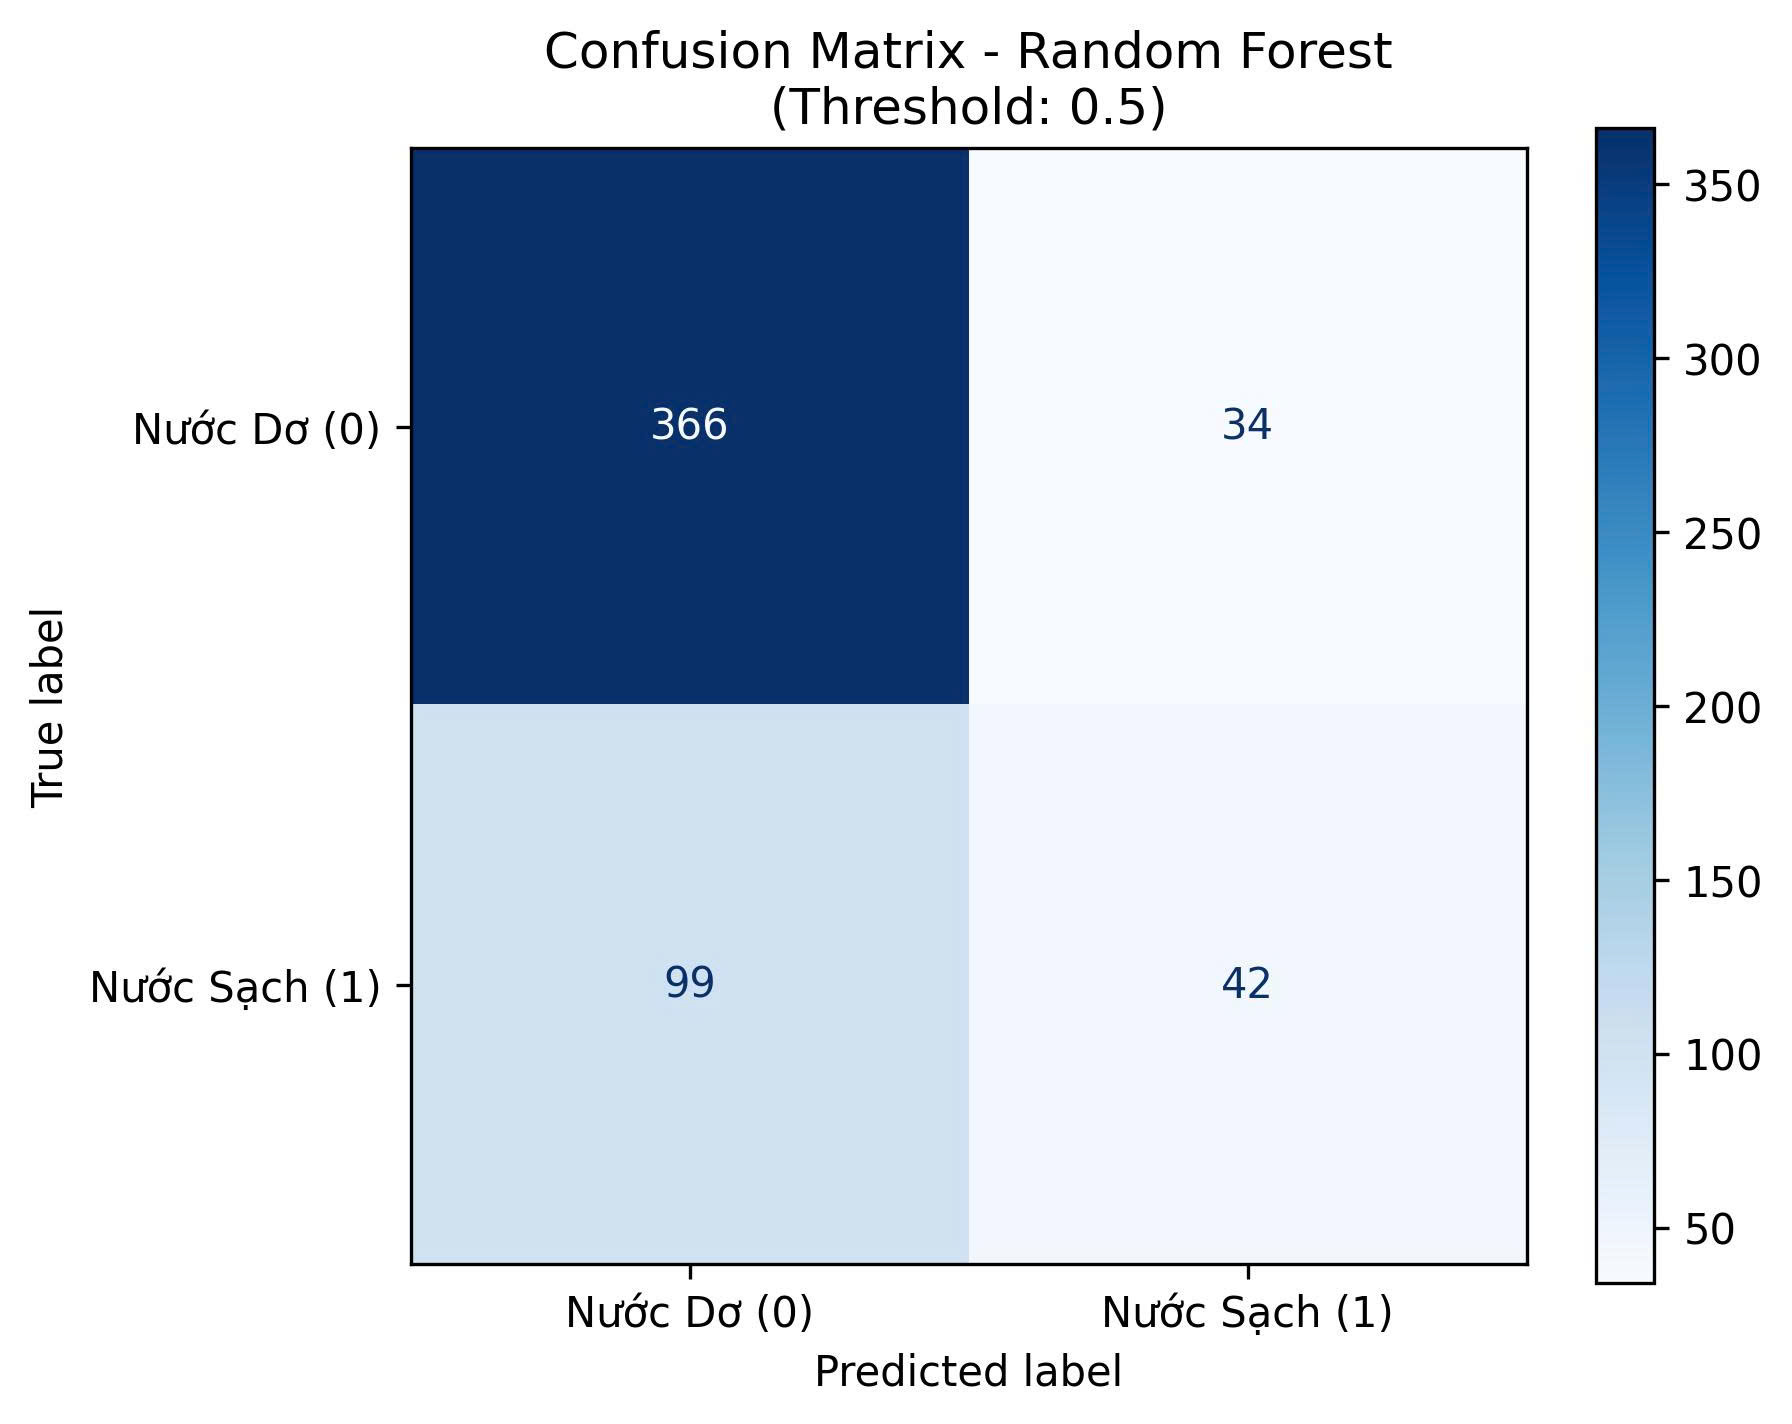
\includegraphics[width=0.6\textwidth]{IMAGE-MODELS/ConfusionMatrix_RandomForest.jpg}
    \caption{Confusion Matrix của mô hình Random Forest tại ngưỡng 0.5}
    \label{fig:cm_rf}
\end{figure}

\subsubsection{Giải thuật XGBoost (Extreme Gradient Boosting)}
\begin{table}[H]
    \centering
    \renewcommand{\arraystretch}{1.2}
    \begin{tabular}{ccccc}
        \hline
        \textbf{Threshold} & \textbf{Precision} & \textbf{Recall} & \textbf{F1-Score} & \textbf{Accuracy} \\
        \hline
        \color{red}0.50 &\color{red} 0.8182 &\color{red} 0.0638 &\color{red} 0.1184 &\color{red} 0.7523 \\

        0.55 & 1.0000 & 0.0426 & 0.0816 & 0.7505 \\

        0.60 & 0.0000 & 0.0000 & 0.0000 & 0.7394 \\

        0.65 & 0.0000 & 0.0000 & 0.0000 & 0.7394 \\

        0.70 & 0.0000 & 0.0000 & 0.0000 & 0.7394 \\

        0.75 & 0.0000 & 0.0000 & 0.0000 & 0.7394 \\

        0.80 & 0.0000 & 0.0000 & 0.0000 & 0.7394 \\
        \hline
    \end{tabular}
    \caption{Kết quả đo lường hiệu suất của mô hình XGBoost qua các ngưỡng}
    \label{tab:xgb_metrics}
\end{table}
Đối với XGBoost, tổ hợp tham số tốt nhất được hệ thống lựa chọn là: \texttt{learning\_rate=0.01}, \texttt{n\_estimators=100}, \texttt{max\_depth=7}, và \texttt{subsample=0.9}. 

Kết quả thực nghiệm cho thấy XGBoost có hành vi phân lớp khá cực đoan. Tại ngưỡng $0.5$, mô hình đạt Precision rất cao lên tới $0.8182$, tuy nhiên chỉ số Recall lại rớt xuống mức cực thấp là $0.0638$ (F1-Score chỉ đạt $0.1184$). Điều này phản ánh việc XGBoost dự đoán vô cùng "thận trọng": nó hiếm khi gán nhãn một mẫu nước là an toàn (1), nhưng một khi đã gán thì tỷ lệ đúng là rất cao. Dù Accuracy vẫn ở mức $75.23\%$, khả năng phát hiện các mẫu nước sạch của XGBoost thực tế bị hạn chế nghiêm trọng.

\begin{figure}[H]
    \centering
    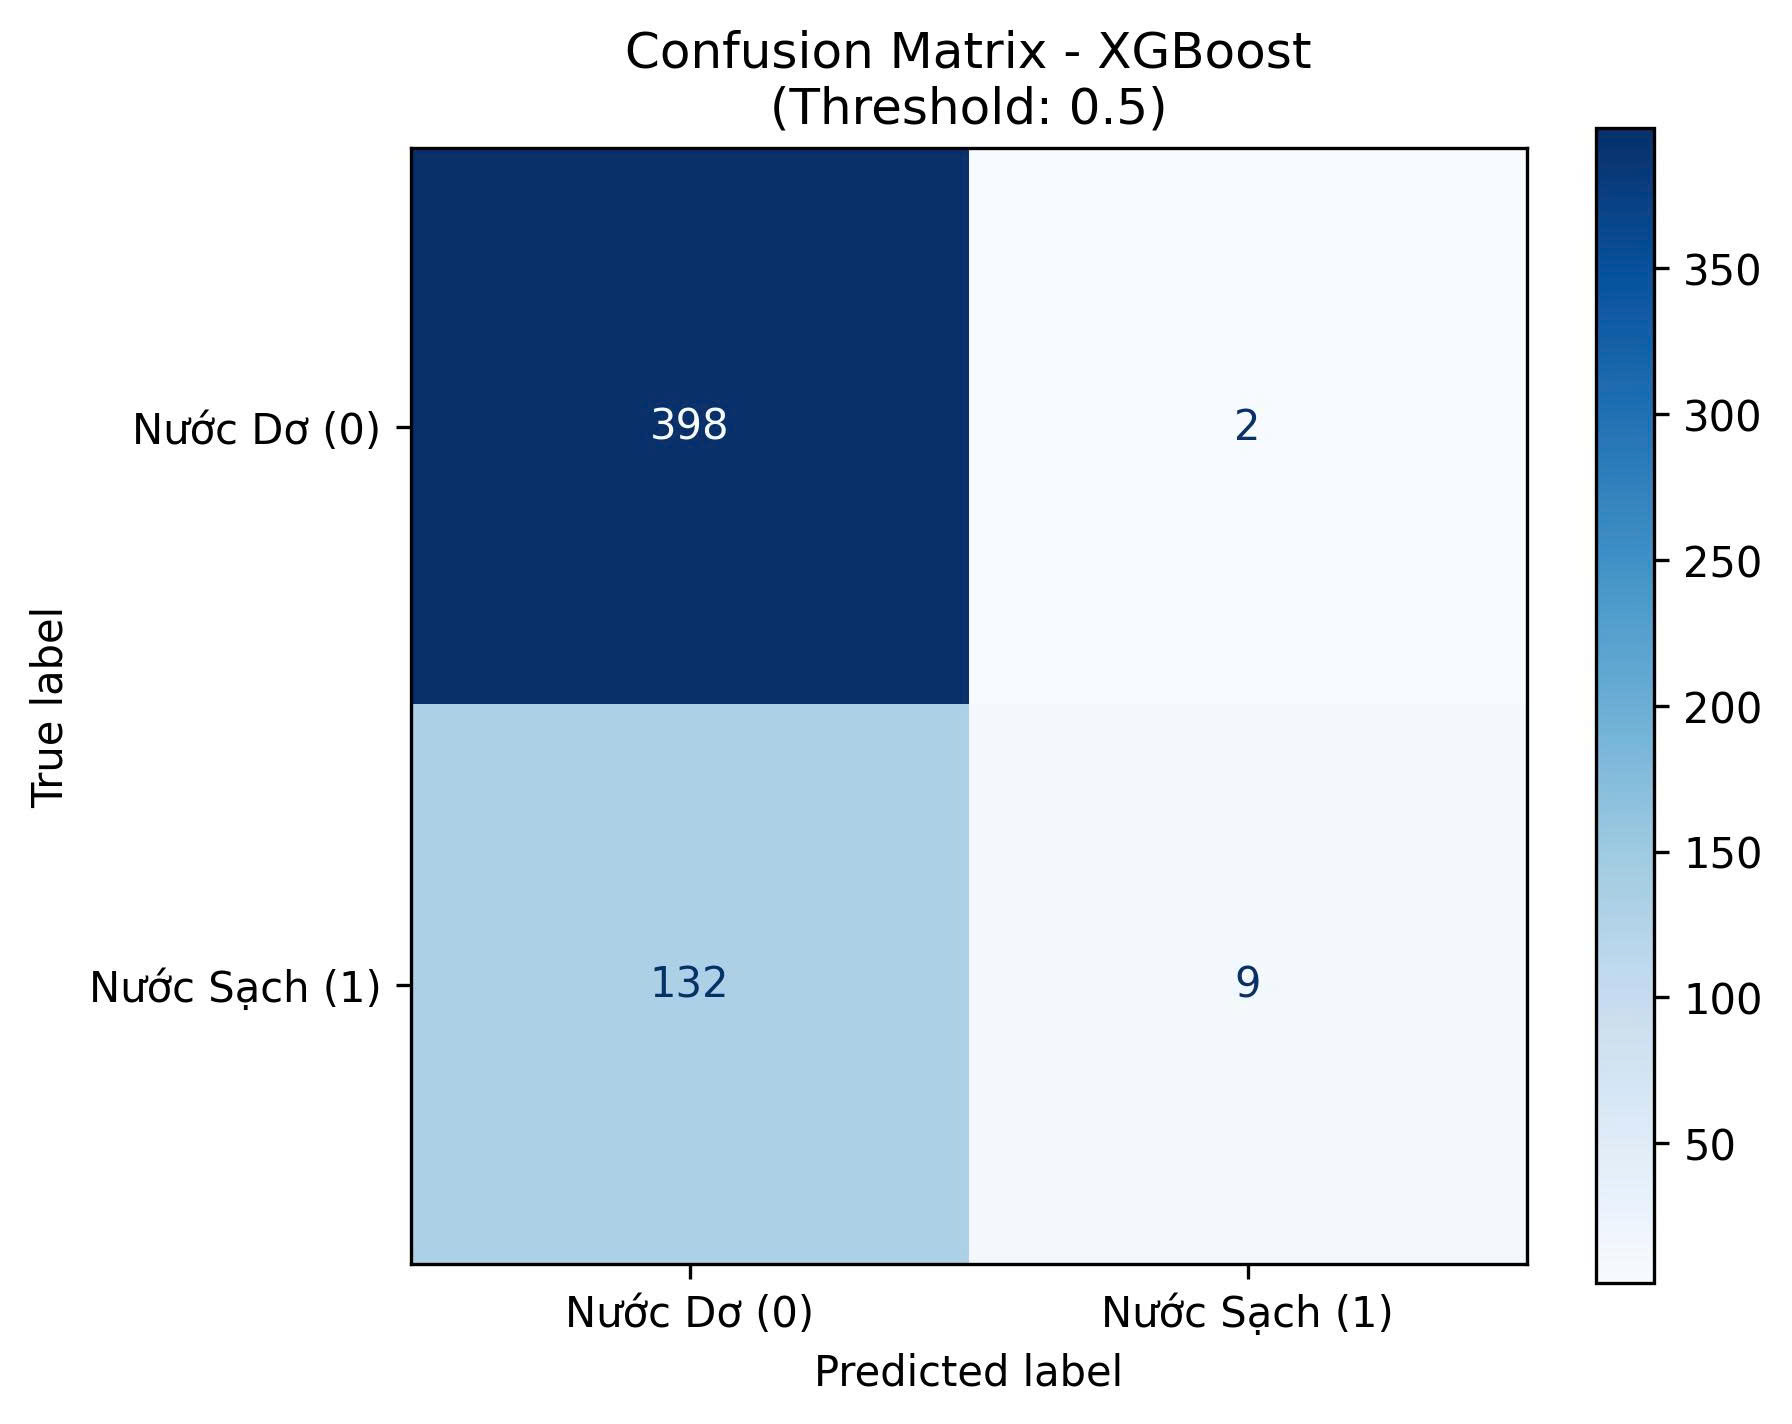
\includegraphics[width=0.6\textwidth]{IMAGE-MODELS/ConfusionMatrix_XGBoost.jpg}
    \caption{Confusion Matrix của mô hình XGBoost tại ngưỡng 0.5}
    \label{fig:cm_xgb}
\end{figure}

\subsubsection{Giải thuật Support Vector Machine (SVM)}
\begin{table}[H]
    \centering
    \renewcommand{\arraystretch}{1.2}
    \begin{tabular}{ccccc}
        \hline
        \textbf{Threshold} & \textbf{Precision} & \textbf{Recall} & \textbf{F1-Score} & \textbf{Accuracy} \\
        \hline
        \color{red}0.50 &\color{red} 0.5345 &\color{red} 0.2199 &\color{red} 0.3116 &\color{red} 0.7468 \\

        0.55 & 0.6080 & 0.1915 & 0.2903 & 0.7568 \\

        0.60 & 0.6410 & 0.1773 & 0.2770 & 0.7597 \\

        0.65 & 0.6471 & 0.1560 & 0.2514 & 0.7579 \\

        0.70 & 0.6097 & 0.1418 & 0.2353 & 0.7597 \\

        0.75 & 0.6900 & 0.1206 & 0.2040 & 0.7560 \\

        0.80 & 0.7500 & 0.0993 & 0.1758 & 0.7560 \\
        \hline
    \end{tabular}
    \caption{Kết quả đo lường hiệu suất của mô hình SVM qua các ngưỡng}
    \label{tab:svm_metrics}
\end{table}
Mô hình SVM được huấn luyện sử dụng nhân RBF phi tuyến trên tập dữ liệu đã qua tiền xử lý chuẩn hóa (\texttt{StandardScaler}). Tại ngưỡng $0.5$, SVM ghi nhận độ chính xác tổng thể (Accuracy) đạt $74.68\%$. Chỉ số Precision ghi nhận ở mức $0.5345$ và Recall là $0.2199$, cho F1-Score tương ứng là $0.3116$.

\begin{figure}[H]
    \centering
    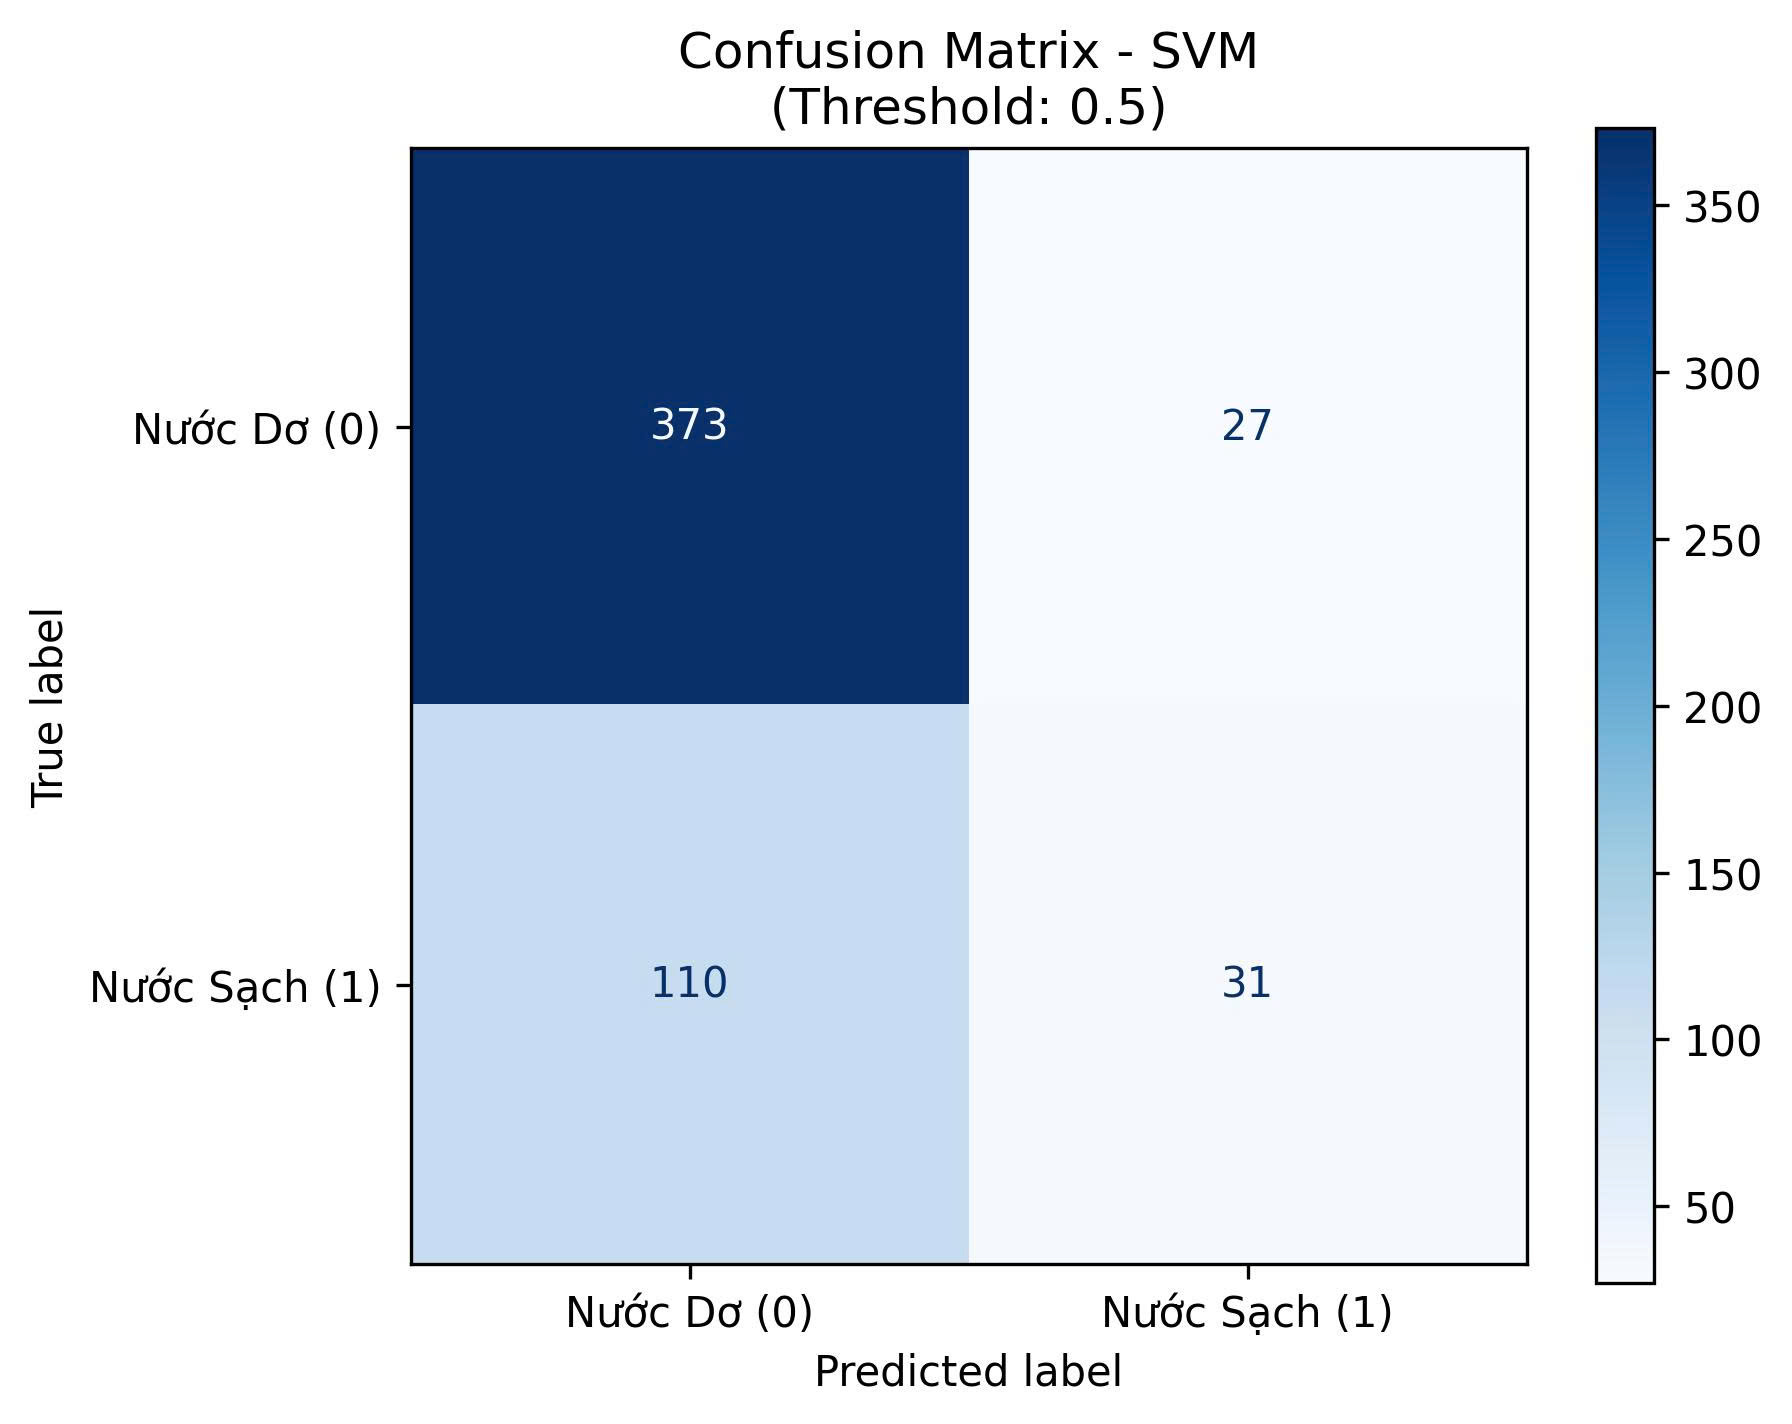
\includegraphics[width=0.6\textwidth]{IMAGE-MODELS/ConfusionMatrix_SVM.jpg}
    \caption{Confusion Matrix của mô hình SVM tại ngưỡng 0.5}
    \label{fig:cm_svm}
\end{figure}

\subsection{Đánh giá tổng quan và lựa chọn mô hình triển khai}

Từ các kết quả đo lường trên, có thể thấy Random Forest và Support Vector Machine (SVM) có hiệu suất phân lớp tương đương nhau (Accuracy đều xoay quanh mốc $75\%$). Tuy nhiên, xét trên bức tranh tổng thể về kỹ thuật và khả năng ứng dụng thực tế, nhóm quyết định lựa chọn Random Forest làm mô hình chính thức để đóng gói và triển khai. Quyết định này được củng cố bởi các luận điểm cốt lõi sau:

\begin{itemize}
    \item \textbf{Hiệu suất cân bằng (F1-Score):} Bài toán có sự chênh lệch dữ liệu dẫn đến việc Accuracy không phản ánh được toàn bộ vấn đề. Xét trên F1-Score (thước đo dung hòa giữa Precision và Recall), Random Forest ($0.3871$) thể hiện khả năng nhận diện nguồn nước sạch nhỉnh hơn hẳn so với SVM ($0.3116$).
    
    \item \textbf{Tối ưu chi phí tiền xử lý (Preprocessing Overhead):} Thuật toán SVM cực kỳ nhạy cảm với thang đo của dữ liệu, bắt buộc hệ thống phải trải qua bước \texttt{StandardScaler} để đưa các đặc trưng về cùng một phân phối. Ngược lại, Random Forest là thuật toán dựa trên phân chia nhánh cây (Tree-based), hoàn toàn "miễn nhiễm" với sự chênh lệch đơn vị đo lường. Lựa chọn Random Forest giúp hệ thống rút ngắn được một khâu tiền xử lý, tăng tốc độ dự đoán (Inference time) khi triển khai luồng dữ liệu thực tế.
    
    \item \textbf{Tối ưu hóa không gian lưu trữ và bộ nhớ (Model Size \& Memory):} Quá trình dự đoán của SVM đòi hỏi phải lưu trữ lại rất nhiều điểm Vector Hỗ trợ (Support Vectors) từ tập huấn luyện. Với một bộ dữ liệu phân tán phức tạp như tính chất hóa lý của nước, file lưu trữ \texttt{.pkl} của SVM thường bị "phình to" về mặt dung lượng. Hơn nữa, để đưa lên môi trường sản phẩm (Production), hệ thống phải tải cùng lúc cả file \texttt{Scaler.pkl} và \texttt{Model.pkl}. Trái lại, Random Forest chỉ cần một tệp trọng số duy nhất, cấu trúc gọn nhẹ, ít tiêu tốn tài nguyên RAM của máy chủ lưu trữ (Server), đáp ứng hoàn hảo tiêu chí của một ứng dụng dự đoán nhanh.
\end{itemize}
\newpage
\section{Trực quan hóa dữ liệu}

% ================= SUBSECTION 1 =================
\subsection{Tổng quan bộ dữ liệu}
% Gom 2 hình tổng quan Dashboard, biểu đồ tròn và phân bố pH vào chung 1 mục

\begin{figure}[H]
    \centering
    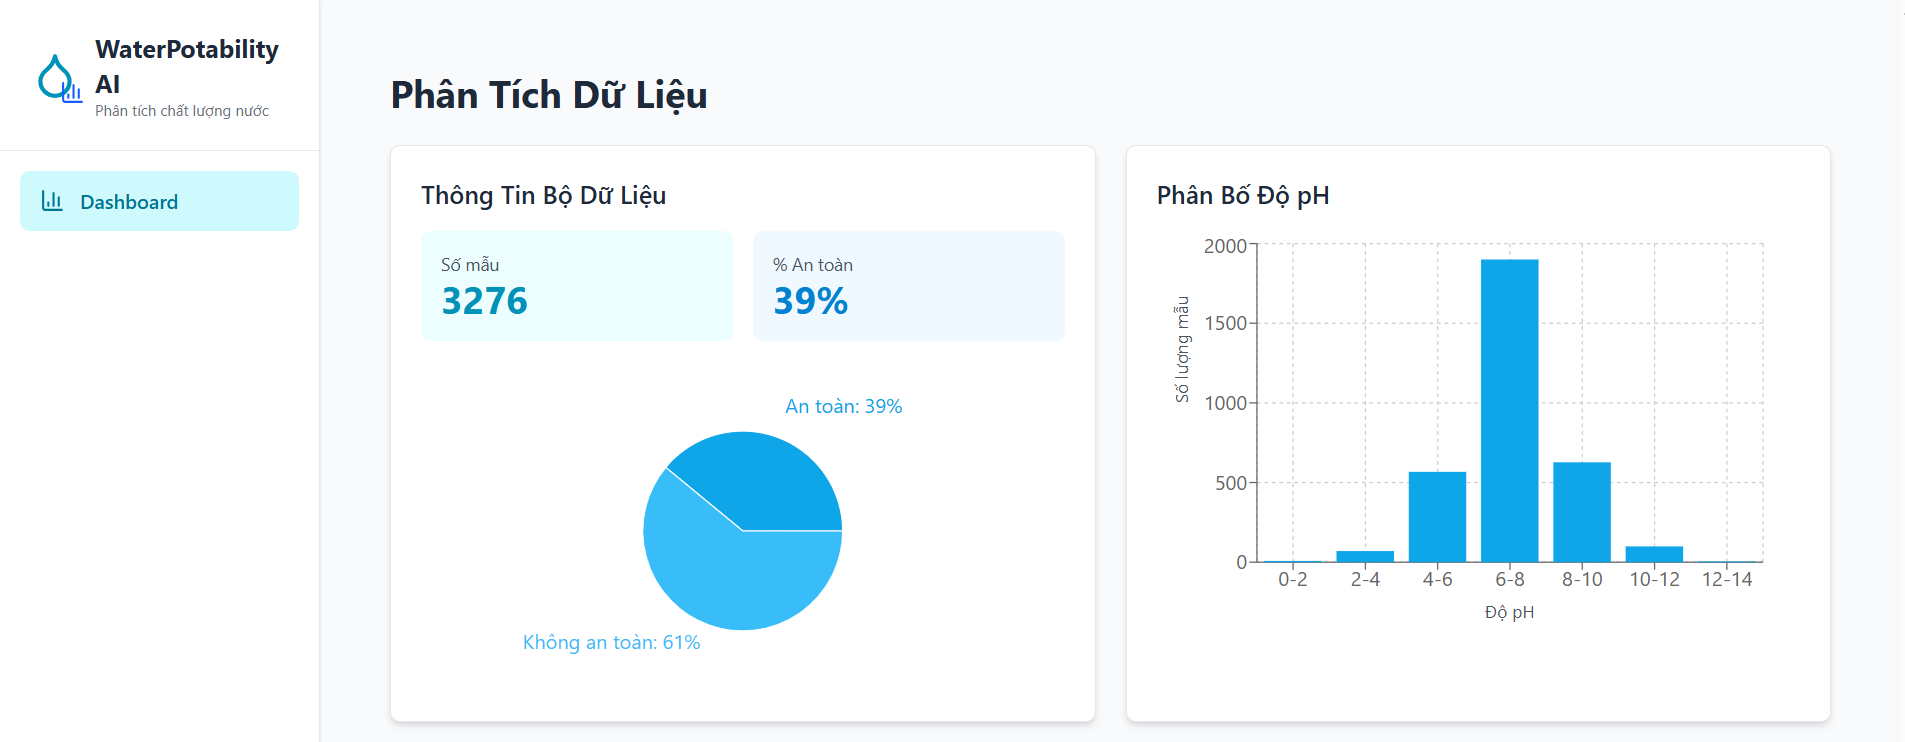
\includegraphics[width=0.9\textwidth]{IMAGE-PENTAHO/pentaho-1.png}
    \caption{Giao diện tổng quan phần Phân tích dữ liệu hiển thị thông tin bộ dữ liệu, biểu đồ tròn tỷ lệ an toàn (được làm nổi bật phần trăm) và biểu đồ cột biểu diễn phân bố độ pH.}
    \label{fig:pentaho_1}
\end{figure}

\begin{figure}[H]
    \centering
    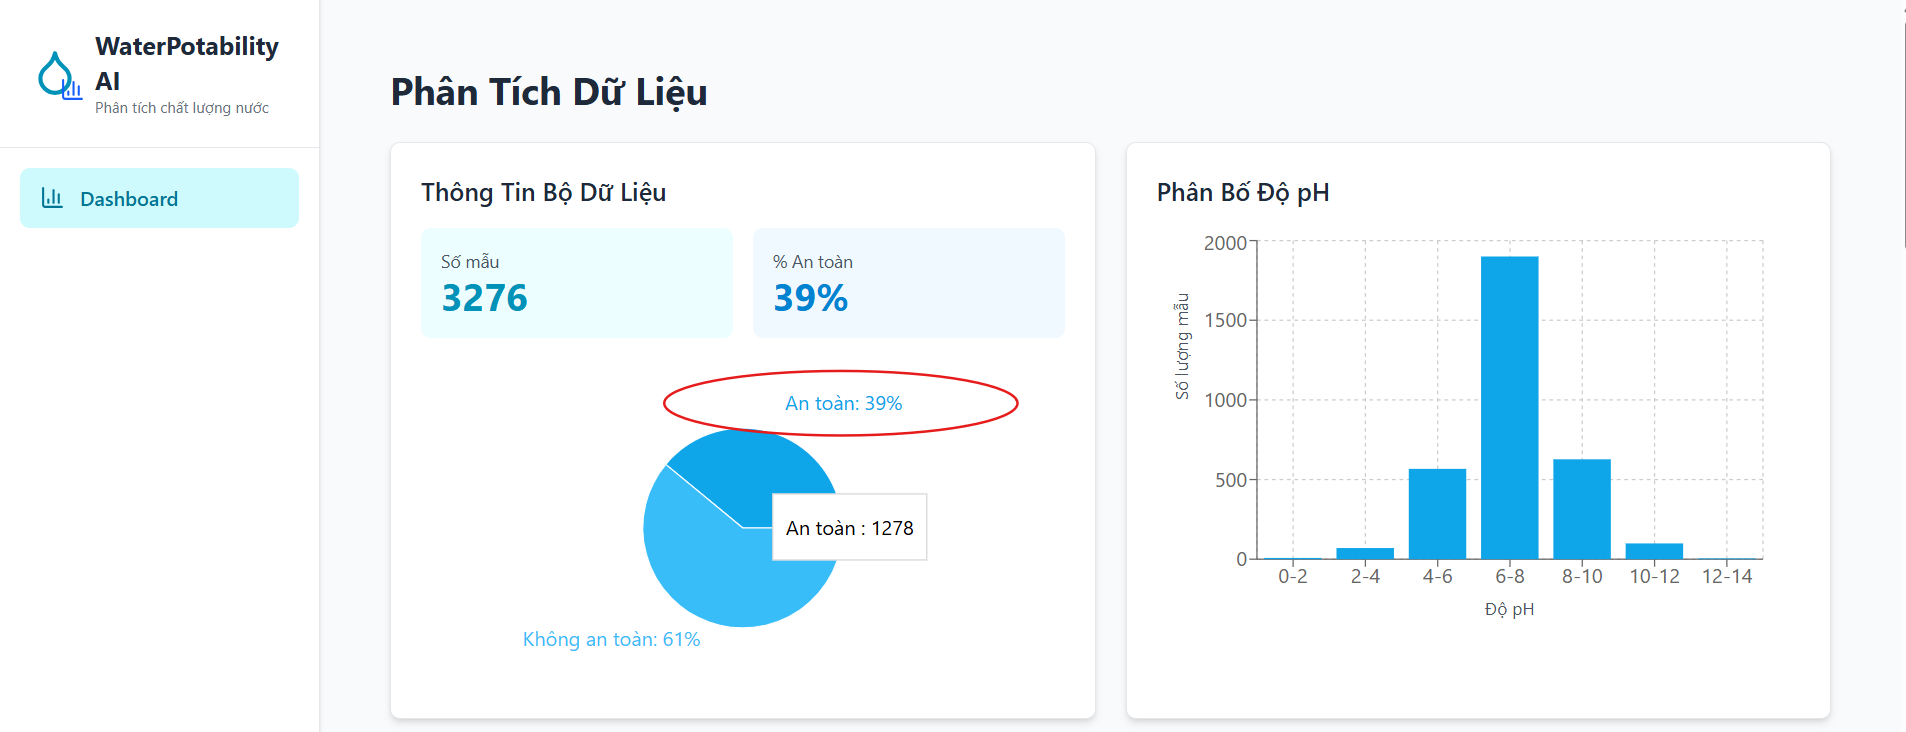
\includegraphics[width=0.9\textwidth]{IMAGE-PENTAHO/pentaho-6.png}
    \caption{Giao diện tổng quan Dashboard thể hiện chi tiết số liệu của bộ dữ liệu gốc bao gồm tổng số mẫu, tỷ lệ phần trăm mẫu nước an toàn/không an toàn và phân bố dữ liệu theo độ pH.}
    \label{fig:pentaho_6}
\end{figure}

% ================= SUBSECTION 2 =================
\subsection{Phân tích phân bố đặc trưng và Tương quan dữ liệu}
% Gom biểu đồ phân bố tứ phân vị (Độ cứng) và Ma trận tương quan Pearson

\begin{figure}[H]
    \centering
    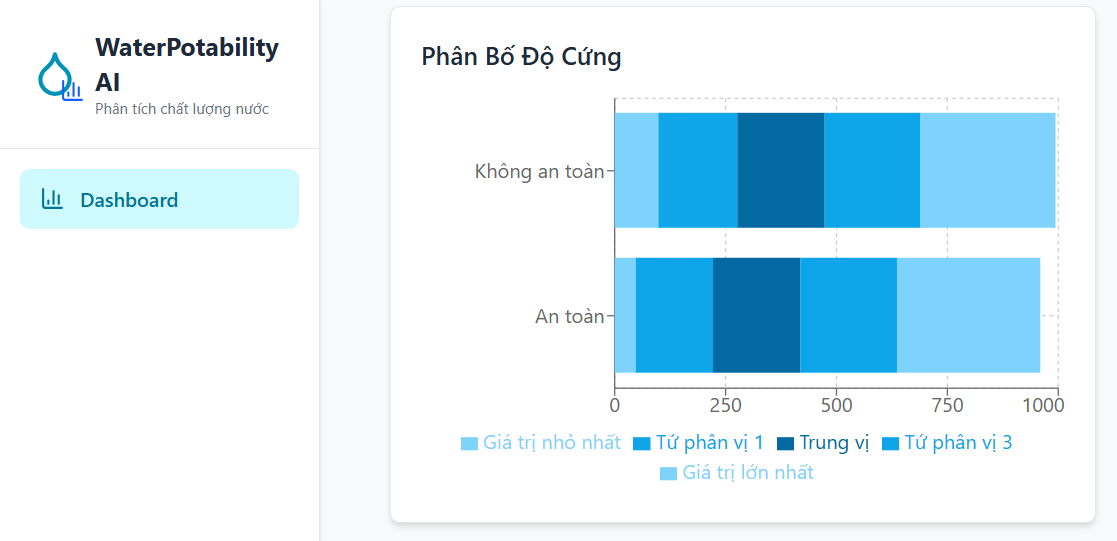
\includegraphics[width=0.9\textwidth]{IMAGE-PENTAHO/phân-bổ-độ-cứng.png}
    \caption{Giao diện trực quan hóa dữ liệu hiển thị biểu đồ phân bố độ cứng (kèm chú giải chi tiết các tứ phân vị, giá trị lớn nhất/nhỏ nhất).}
    \label{fig:phan_bo_do_cung}
\end{figure}

\begin{figure}[H]
    \centering
    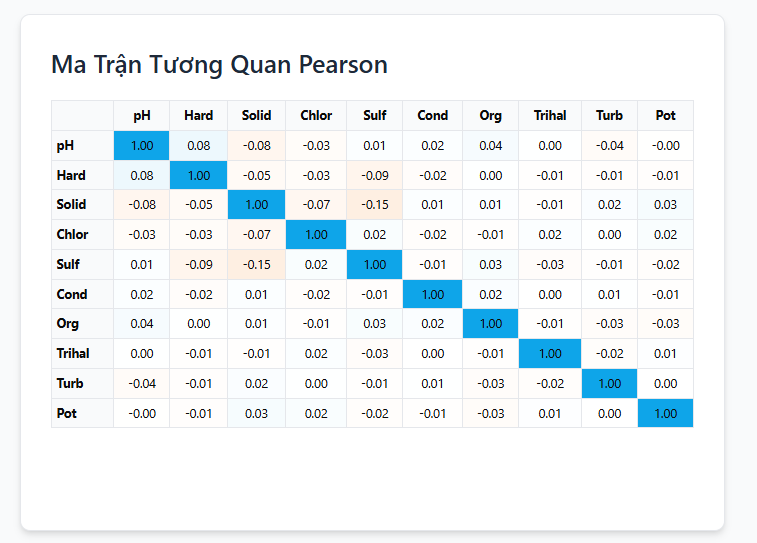
\includegraphics[width=0.9\textwidth]{IMAGE-PENTAHO/pearson.png}
    \caption{Ma trận tương quan Pearson giữa các chỉ số.}
    \label{fig:pearson_matrix}
\end{figure}

% ================= SUBSECTION 3 =================
\subsection{Phân tích mối quan hệ đa biến}
% Gom các biểu đồ phân tán (Scatter plot) và so sánh trung bình giữa 2 nhãn An toàn/Không an toàn

\begin{figure}[H]
    \centering
    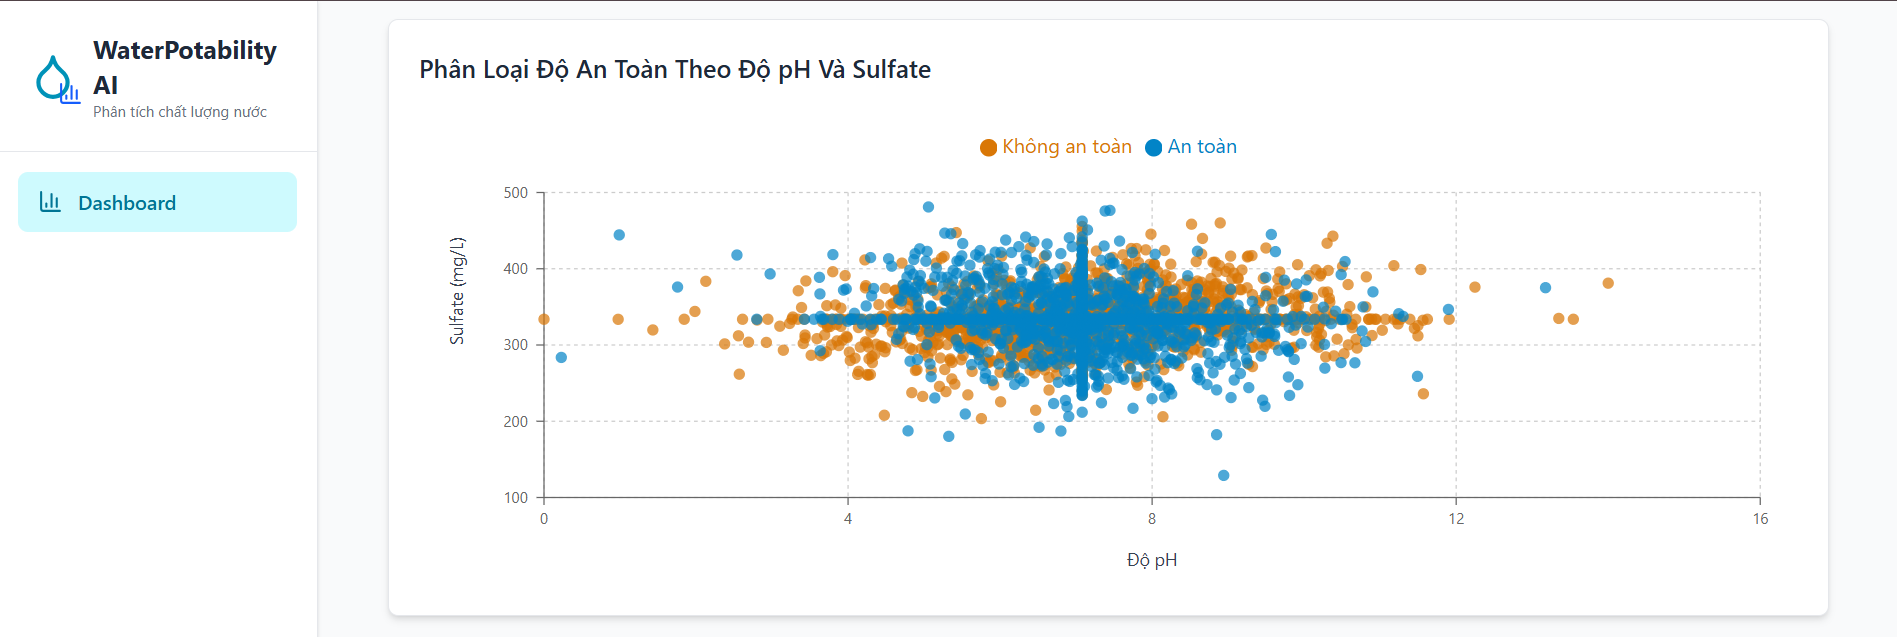
\includegraphics[width=0.9\textwidth]{IMAGE-PENTAHO/phân-loại-an-toàn.png}
    \caption{Biểu đồ phân tán (Scatter plot) thể hiện mối quan hệ và sự phân loại độ an toàn của nguồn nước dựa trên hai đặc trưng: độ pH và Sulfate.}
    \label{fig:phan_loai_an_toan}
\end{figure}

\begin{figure}[H]
    \centering
    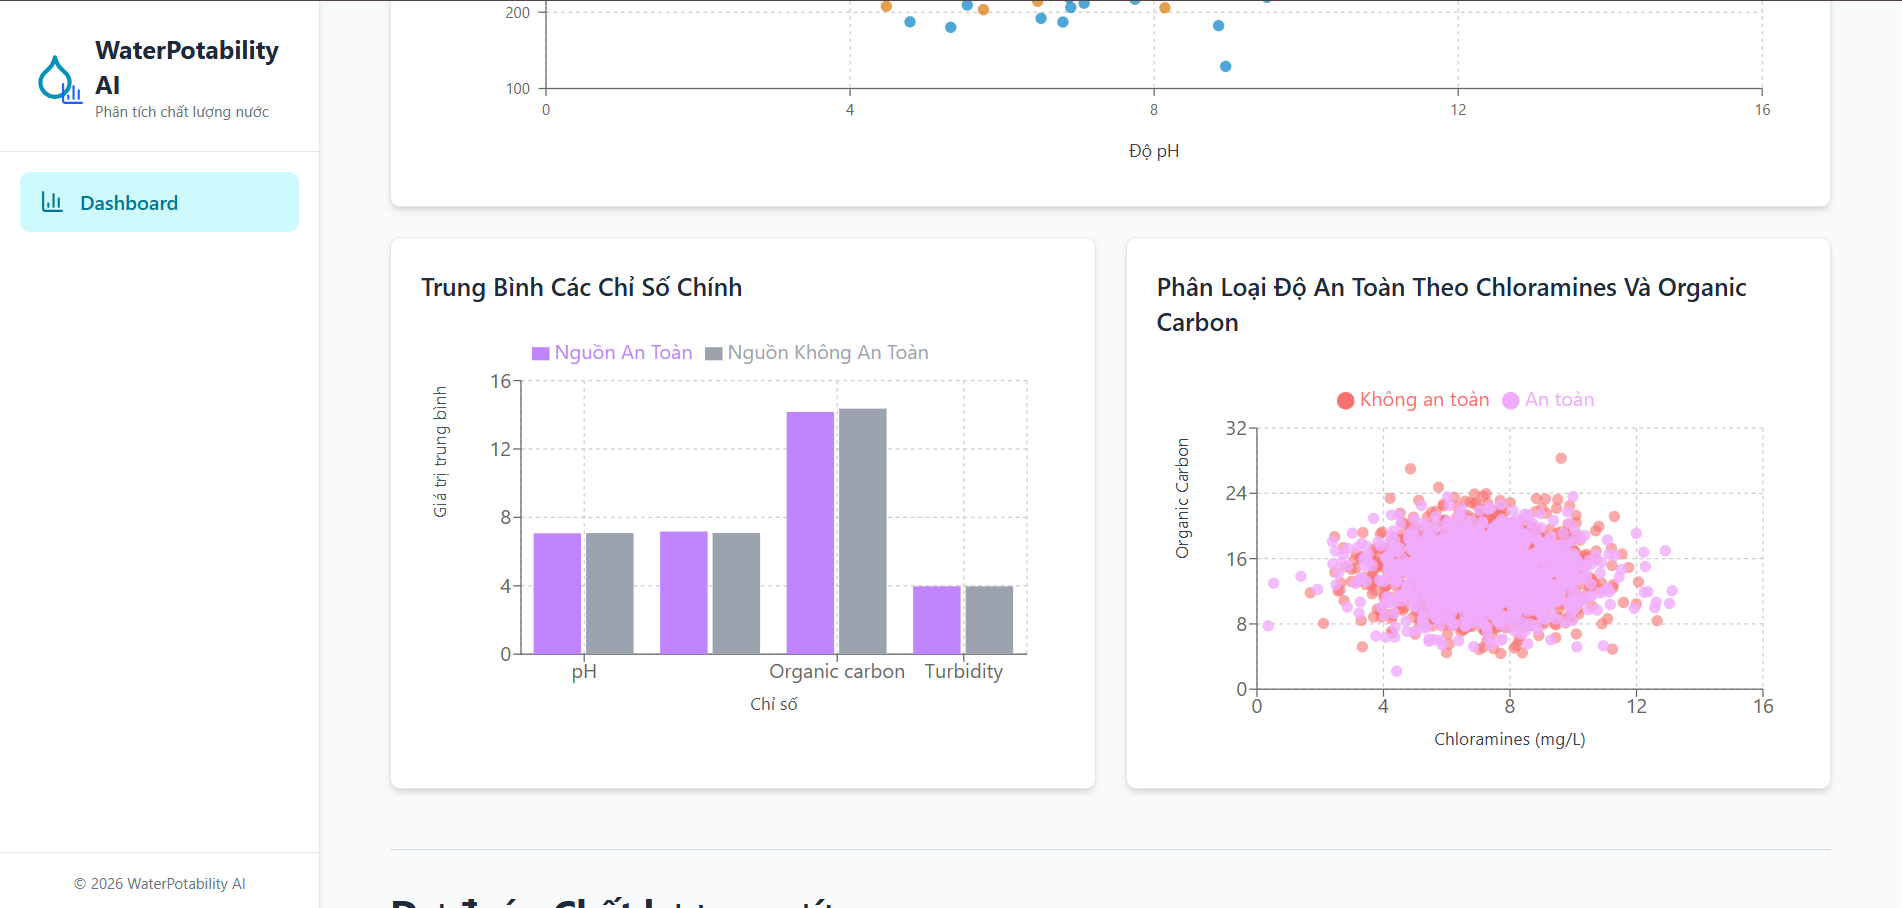
\includegraphics[width=0.9\textwidth]{IMAGE-PENTAHO/pentaho-4.png}
    \caption{Giao diện so sánh giá trị trung bình của các chỉ số chính (pH, Organic carbon, Turbidity) giữa hai nhóm an toàn/không an toàn và biểu đồ phân loại theo Chloramines và Organic Carbon.}
    \label{fig:pentaho_4}
\end{figure}

% ================= SUBSECTION 4 =================
\subsection{Giao diện dự đoán và Đánh giá mô hình}
% Tách riêng phần Demo giao diện dự đoán và các chỉ số (Accuracy, F1,...)

\begin{figure}[H]
    \centering
    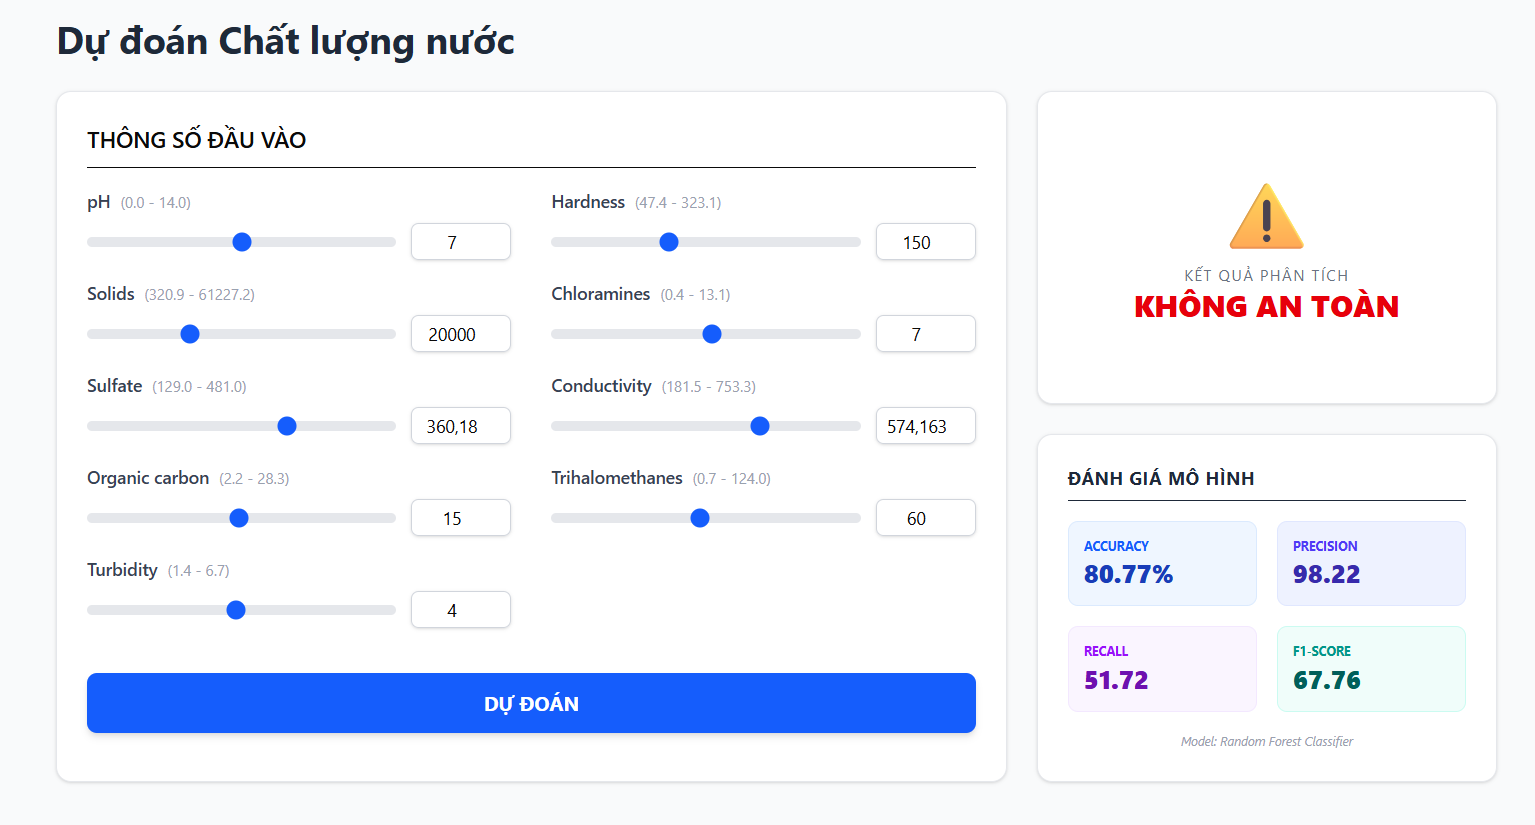
\includegraphics[width=0.9\textwidth]{IMAGE-PENTAHO/pentaho-5.png}
    \caption{Giao diện Dự đoán chất lượng nước cho phép người dùng tùy chỉnh các thông số đầu vào, hiển thị kết quả phân tích trực quan và các chỉ số đánh giá hiệu suất của mô hình (Accuracy, Precision, Recall, F1-Score).}
    \label{fig:pentaho_5}
\end{figure}
\newpage
\section{Kết luận và Hướng phát triển tương lai}

\subsection{Kết luận}
Bài tập lớn đã nghiên cứu và thiết kế và triển khai thành công một quy trình hoàn chỉnh từ khâu thu thập, tiền xử lý dữ liệu (ETL), xây dựng Kho dữ liệu (Data Warehouse) đến việc phân tích trực quan và tích hợp mô hình Học máy dự đoán chất lượng nước (Water Potability). Bằng việc kết hợp các công cụ chuyên dụng như Pentaho và các thuật toán học máy, đồ án đã giải quyết tốt bài toán đánh giá độ an toàn của nguồn nước. Các kết quả nổi bật mà nhóm đã đạt được bao gồm:

\begin{enumerate}[label=\textbf{\arabic*.}]
    \item \textbf{Xây dựng thành công quy trình ETL và Kho dữ liệu:} Hệ thống đã xử lý và làm sạch bộ dữ liệu gốc, giải quyết triệt để các giá trị khuyết thiếu (như độ pH, Sulfate) bằng kỹ thuật điền khuyết trung bình (Mean Imputation). Từ đó, nhóm đã thiết kế và đổ dữ liệu thành công vào mô hình Đa chiều (Star Schema) với bảng Fact và các bảng Dimension, giúp tối ưu hóa việc lưu trữ và truy vấn phục vụ phân tích.
    
    \item \textbf{Trực quan hóa và phân tích dữ liệu (EDA) sâu sắc:} Thông qua các Dashboard trực quan, nhóm đã khám phá ra tính phi tuyến tính phức tạp của tập dữ liệu. Phân tích chỉ ra rằng không có một ngưỡng cố định đơn lẻ nào (như chỉ dựa vào độ pH hay Sulfate) có thể quyết định hoàn toàn độ an toàn của nước. Khám phá này là tiền đề định lượng vững chắc để áp dụng các mô hình AI có khả năng học được các biểu diễn phức tạp.
    
    \item \textbf{Triển khai mô hình Học máy dự đoán chất lượng nước:} Đồ án đã áp dụng và đánh giá thành công các thuật toán phân loại mạnh mẽ (như Random Forest, SVM, XGBoost). Các mô hình đã nắm bắt tốt sự tương tác đa chiều giữa 9 chỉ số hóa lý của nước, đưa ra kết quả dự đoán (An toàn / Không an toàn) với các chỉ số đánh giá độ chính xác (Accuracy, Precision, Recall, F1-Score) tương đối khả quan.
    
    \item \textbf{Xây dựng giao diện Web tương tác trực quan:} Thay vì chỉ dừng lại ở các đoạn mã (code) mô hình tĩnh, nhóm đã xây dựng thành công một ứng dụng Web cho phép người dùng điều chỉnh trực tiếp các thông số môi trường nước đầu vào. Hệ thống tích hợp trực tiếp với mô hình đã huấn luyện để trả về kết quả dự đoán tức thời kèm theo các cảnh báo trực quan, minh chứng cho tính ứng dụng thực tiễn cao của đề tài.
\end{enumerate}

\subsection{Hướng phát triển tương lai}
Mặc dù kiến trúc hệ thống đã vận hành ổn định và mô hình đưa ra những dự đoán có giá trị, nhưng do giới hạn về mặt thời gian và tài nguyên, hệ thống vẫn có thể được nâng cấp để tiệm cận với tiêu chuẩn thực tế của doanh nghiệp ở các khía cạnh sau:

\begin{itemize}
    \item \textbf{Xử lý triệt để bài toán mất cân bằng dữ liệu:} Trong tập dữ liệu hiện tại, tỉ lệ mẫu nước Không an toàn (61\%) đang chiếm ưu thế hơn so với nhóm An toàn (39\%). Hướng nâng cấp sắp tới là áp dụng các kỹ thuật sinh mẫu nhân tạo mạnh mẽ hơn (như SMOTE) hoặc tinh chỉnh sâu siêu tham số (Hyperparameter tuning) để tăng độ nhạy (Recall) cho lớp dữ liệu thiểu số, tránh việc mô hình bị thiên lệch.
    
    \item \textbf{Tích hợp luồng dữ liệu thời gian thực từ cảm biến IoT:} Thay vì phụ thuộc vào thao tác nhập liệu thủ công trên giao diện web, hệ thống tương lai có thể được mở rộng để nhận luồng dữ liệu trực tiếp từ các hệ thống cảm biến đo chất lượng nước (IoT Sensors) đặt tại các hồ chứa hoặc trạm bơm. Kết hợp với Apache Kafka, ứng dụng sẽ trở thành một Pipeline cảnh báo ô nhiễm nguồn nước tự động theo thời gian thực (Real-time Alert System).
    
    \item \textbf{Triển khai Đám mây (Cloud Deployment) và MLOps:} Đưa toàn bộ hệ thống (Database, ETL Pipeline, Web App) từ môi trường máy chủ cục bộ lên các nền tảng đám mây như AWS hoặc Google Cloud. Đồng thời, xây dựng quy trình MLOps để mô hình Học máy có thể tự động thu thập dữ liệu mới, tái huấn luyện và cập nhật liên tục, đảm bảo độ chính xác lâu dài trong điều kiện môi trường tự nhiên liên tục biến đổi.
\end{itemize}
\newpage
\phantomsection % Tạo một "mỏ neo" tại vị trí này để hyperref nhận diện
\addcontentsline{toc}{section}{TÀI LIỆU THAM KHẢO}
\section*{TÀI LIỆU THAM KHẢO}

[1] Y.-C. Lee, T.-P. Hong, and W.-Y. Lin, "Mining association rules with multiple minimum supports using maximum constraints," \textit{International Journal of Approximate Reasoning}, vol. 40, pp. 44–54, 2005, doi: 10.1016/j.ijar.2004.11.006.

[2] World Health Organization (WHO), \textit{Guidelines for drinking-water quality}, 4th ed. Geneva, Switzerland: World Health Organization, 2011.

[3] R. Kimball and M. Ross, \textit{The Data Warehouse Toolkit: The Definitive Guide to Dimensional Modeling}, 3rd ed. Indianapolis, IN, USA: Wiley, 2013.

[4] M. Casters, R. Bouman, and J. Van Dongen, \textit{Pentaho Kettle Solutions: Building Open Source ETL Solutions with Pentaho Data Integration}. Indianapolis, IN, USA: Wiley Publishing, 2010.

[5] L. Breiman, "Random forests," \textit{Machine Learning}, vol. 45, no. 1, pp. 5--32, 2001, doi: 10.1023/A:1010933404324.

[6] C. Cortes and V. Vapnik, "Support-vector networks," \textit{Machine Learning}, vol. 20, no. 3, pp. 273--297, 1995, doi: 10.1007/BF00994018.

[7] T. Chen and C. Guestrin, "XGBoost: A scalable tree boosting system," in \textit{Proceedings of the 22nd ACM SIGKDD International Conference on Knowledge Discovery and Data Mining}, 2016, pp. 785--794, doi: 10.1145/2939672.2939785.

[8] N. V. Chawla, K. W. Bowyer, L. O. Hall, and W. P. Kegelmeyer, "SMOTE: Synthetic minority over-sampling technique," \textit{Journal of Artificial Intelligence Research}, vol. 16, pp. 321--357, 2002.

[9] U. Ahmed, R. Mumtaz, H. Anwar, A. A. Shah, R. Tariq, and U. Hassan, "Efficient water quality prediction using supervised machine learning," \textit{Water}, vol. 11, no. 11, p. 2210, 2019, doi: 10.3390/w11112210.

[10] S. K. Singh, P. R. Muduli, S. K. Rath, et al., "Machine learning based system for water potability prediction," in \textit{2021 IEEE International Conference on Communication, Information and Computing Technology (ICCICT)}, 2021, pp. 1--5.

[11] J. Han, M. Kamber, and J. Pei, \textit{Data Mining: Concepts and Techniques}, 3rd ed. Waltham, MA, USA: Morgan Kaufmann, 2011.

[12] F. Pedregosa et al., "Scikit-learn: Machine learning in Python," \textit{Journal of Machine Learning Research}, vol. 12, pp. 2825--2830, 2011.

[13] W. McKinney, "Data structures for statistical computing in Python," in \textit{Proceedings of the 9th Python in Science Conference}, 2010, pp. 51--56.

[14] D. Pyle, \textit{Data Preparation for Data Mining}. San Francisco, CA, USA: Morgan Kaufmann Publishers, 1999.

[15] J. Kreps, N. Narkhede, and J. Rao, "Kafka: A crucial system for log processing in LinkedIn," in \textit{Proceedings of the 4th Biennial Conference on Innovative Data Systems Research (CIDR)}, 2011.
\end{document}
